\documentclass[pregrado]{tesis-usb}

% paquetes
\usepackage[utf8]{inputenc}
\usepackage{verbatim}
\usepackage{acronym}
\usepackage{float}
% \usepackage{hyperref}
\usepackage[spanish]{babel}
\usepackage{amsmath,amsthm,amsfonts,amssymb,amscd}
\usepackage{mathrsfs}
\usepackage{xcolor}
\usepackage{graphicx}
\usepackage{listings}
\usepackage{multicol}
\usepackage{color}
\usepackage{mathdots}
\usepackage{physics}

%New colors defined below
\definecolor{codegreen}{rgb}{0,0.6,0}
\definecolor{codegray}{rgb}{0.5,0.5,0.5}
\definecolor{codepurple}{rgb}{0.58,0,0.82}
\definecolor{backcolour}{rgb}{0.95,0.95,0.92}

% Para arreglar espacio entre parrafos y sangria
\usepackage{parskip}
\setlength{\parindent}{3ex}

% fragmentos de código
\usepackage{listings}
\renewcommand{\lstlistingname}{Fragmento de Código}
\renewcommand{\lstlistlistingname}{Índice de Fragmentos de Código}
\lstset{
	basicstyle=\ttfamily\footnotesize,
	frame=single,
	captionpos=b,
	numbers=left,
	showstringspaces=false,
	aboveskip=1em,
	belowskip=2em,
	xleftmargin=1em,
	xrightmargin=1em,
	tabsize=4}


% estilo de las referencias
\bibliographystyle{plain}

\autor{Siria Sadeddin}
\autori{}
\usbid{08-11245}
\titulo{ Dinámica de partículas de Wannier en campos de fuerza inhomogéneos, periódicos y rápidamente oscilantes}
\fecha{Enero~de~2020}
\agno{2020}
\fechadefensa{27~de~enero~de~2020}
\tutor{Prof. Luis Alfredo Martínez}
\trabajo{Proyecto de Grado}
\coord{Licenciatura en F\'isica} %Coloca la coordinación
\grado{Licenciada en F\'isica} %coloca el postgrado
\carrera{Carrera}
\programa{Maestr\'ia en Matem\'aticas}
\juradouno{Eduardo Pestana}
\juradodos{Gloria Buendía}
\juradotres{Luis Alfredo Martínez}


\makeatletter
\let \@sverbatim \@verbatim
\def \@verbatim {\@sverbatim \verbatimplus}
{\catcode`'=13 \gdef \verbatimplus{\catcode`'=13 \chardef '=13 }} 
\makeatother

\begin{document}

\newtheorem{obs}{Observaci\'on}
\newtheorem{prob}{Problema}
\newtheorem{proy}{Proyecto}
\newtheorem{defi}{Definición}
\newtheorem{prop}{Proposici\'on}
\newtheorem{teo}{Teorema}
\newtheorem{ejem}{Ejemplo}



\maketitle
%\pagestyle{empty}
\begin{figure}
    \centering
    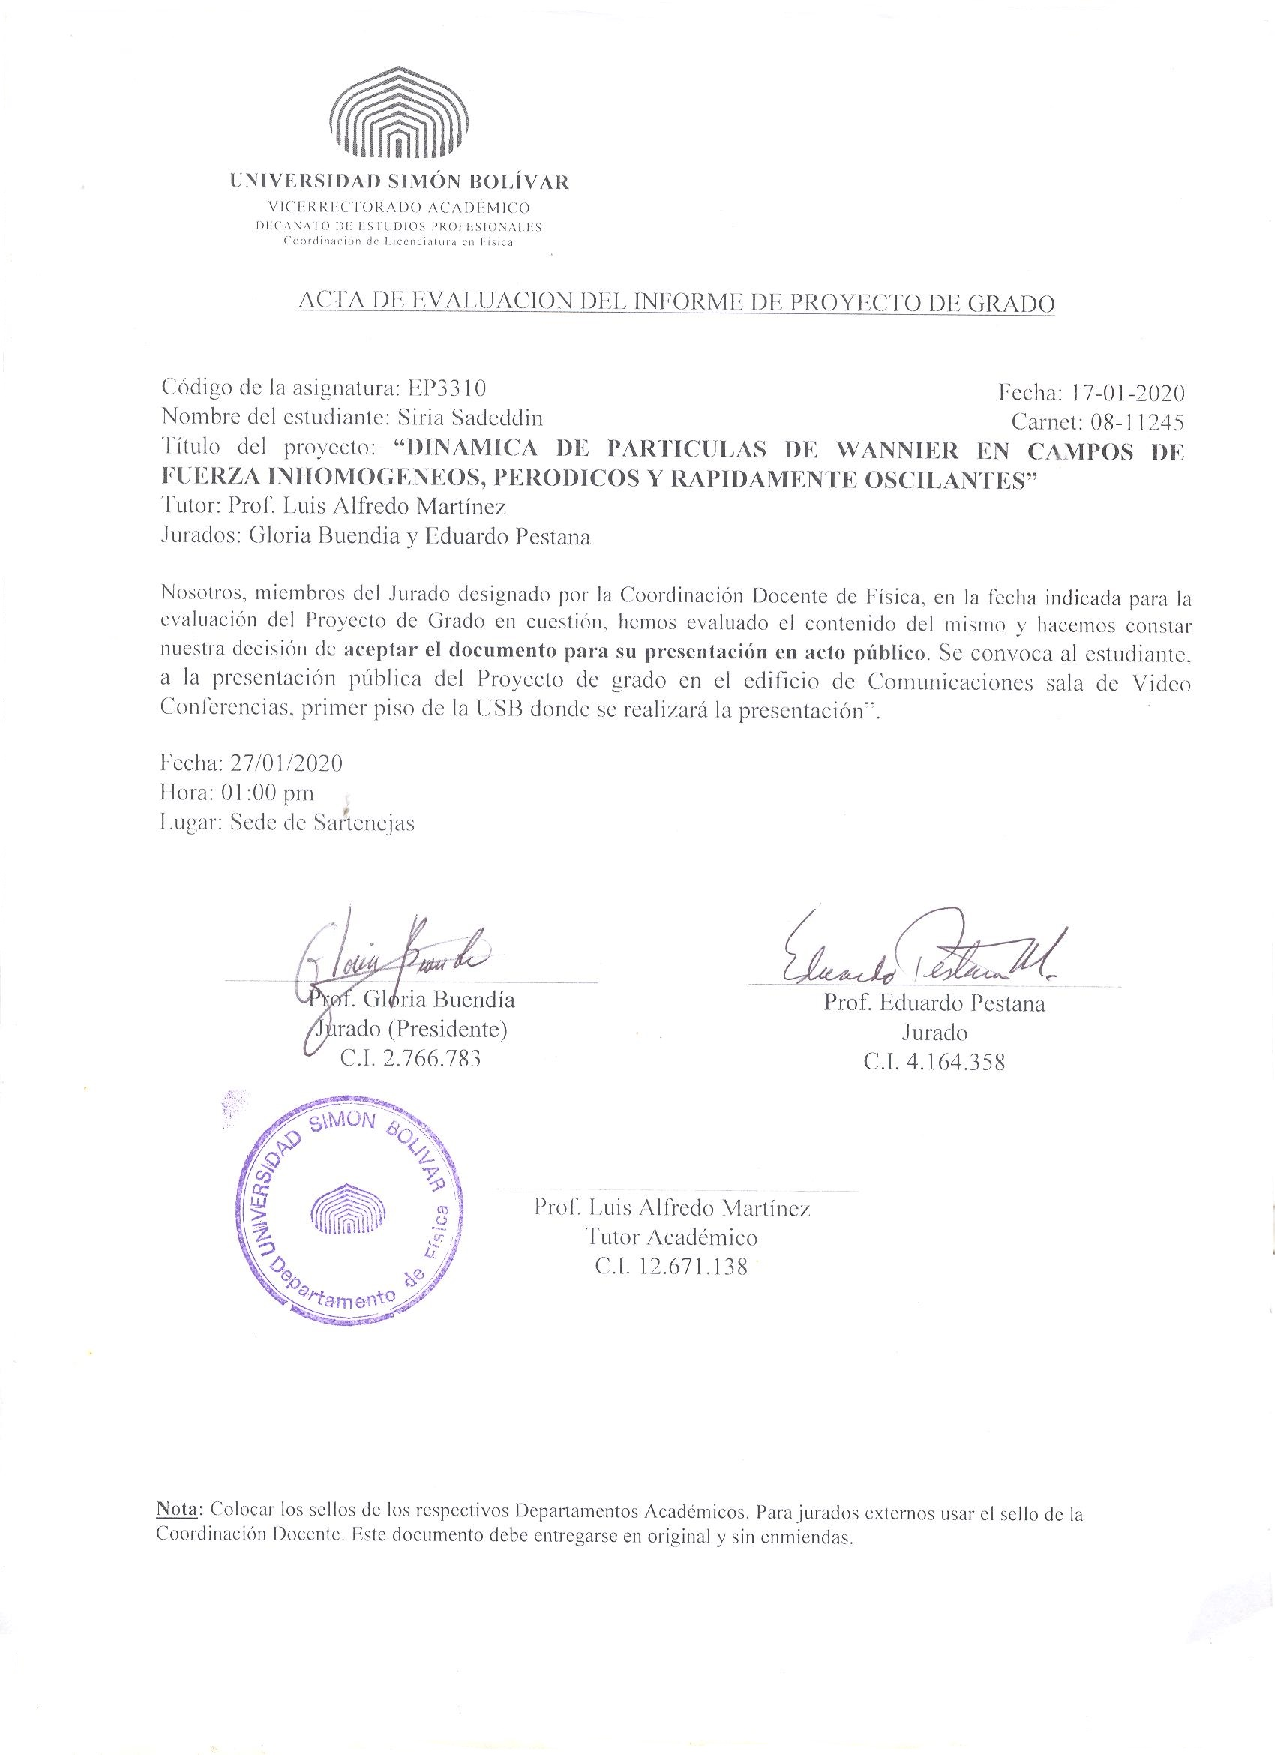
\includegraphics[width=1\columnwidth]{imagenes/ActaevaluacioncontenidoSiria3.pdf}
\end{figure}

%\newpage
%\pagestyle{empty}
\begin{figure}
    \centering
    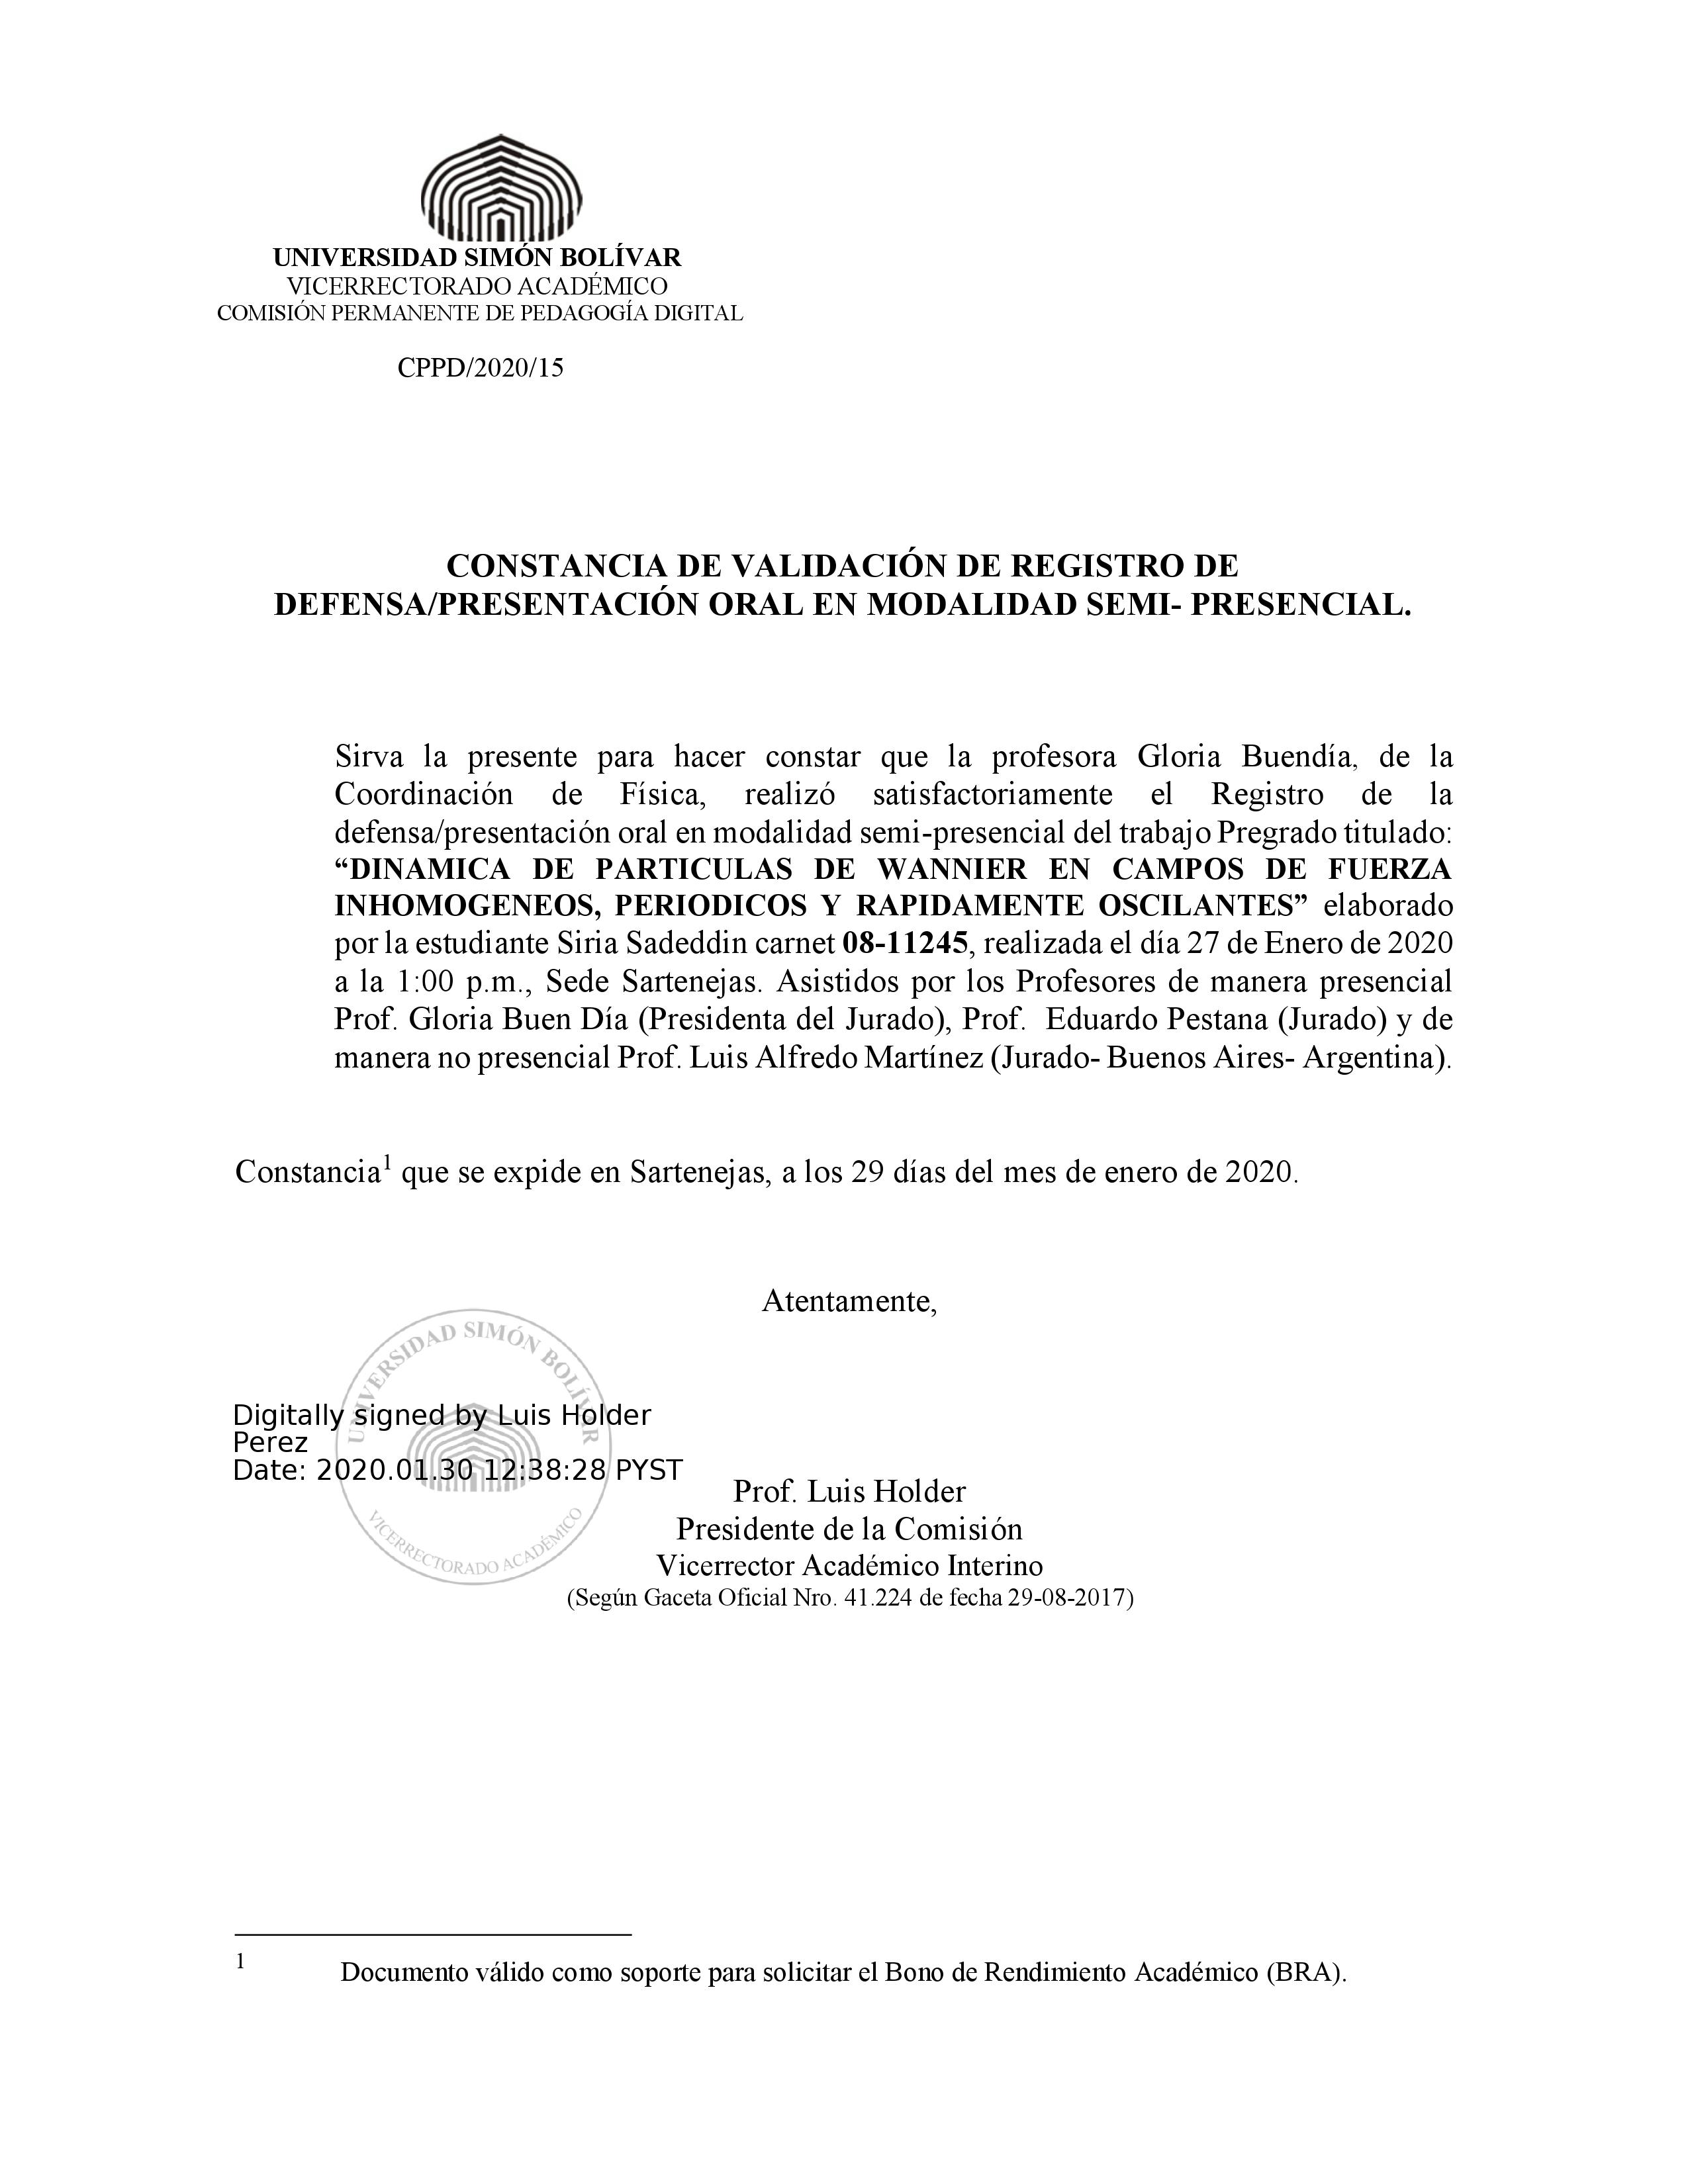
\includegraphics[width=1\columnwidth]{imagenes/ConstanciadefensaTDDSiriaSadeddin.jpg}
\end{figure}

%\newpage
%\pagestyle{empty}
\begin{figure}
    \centering
    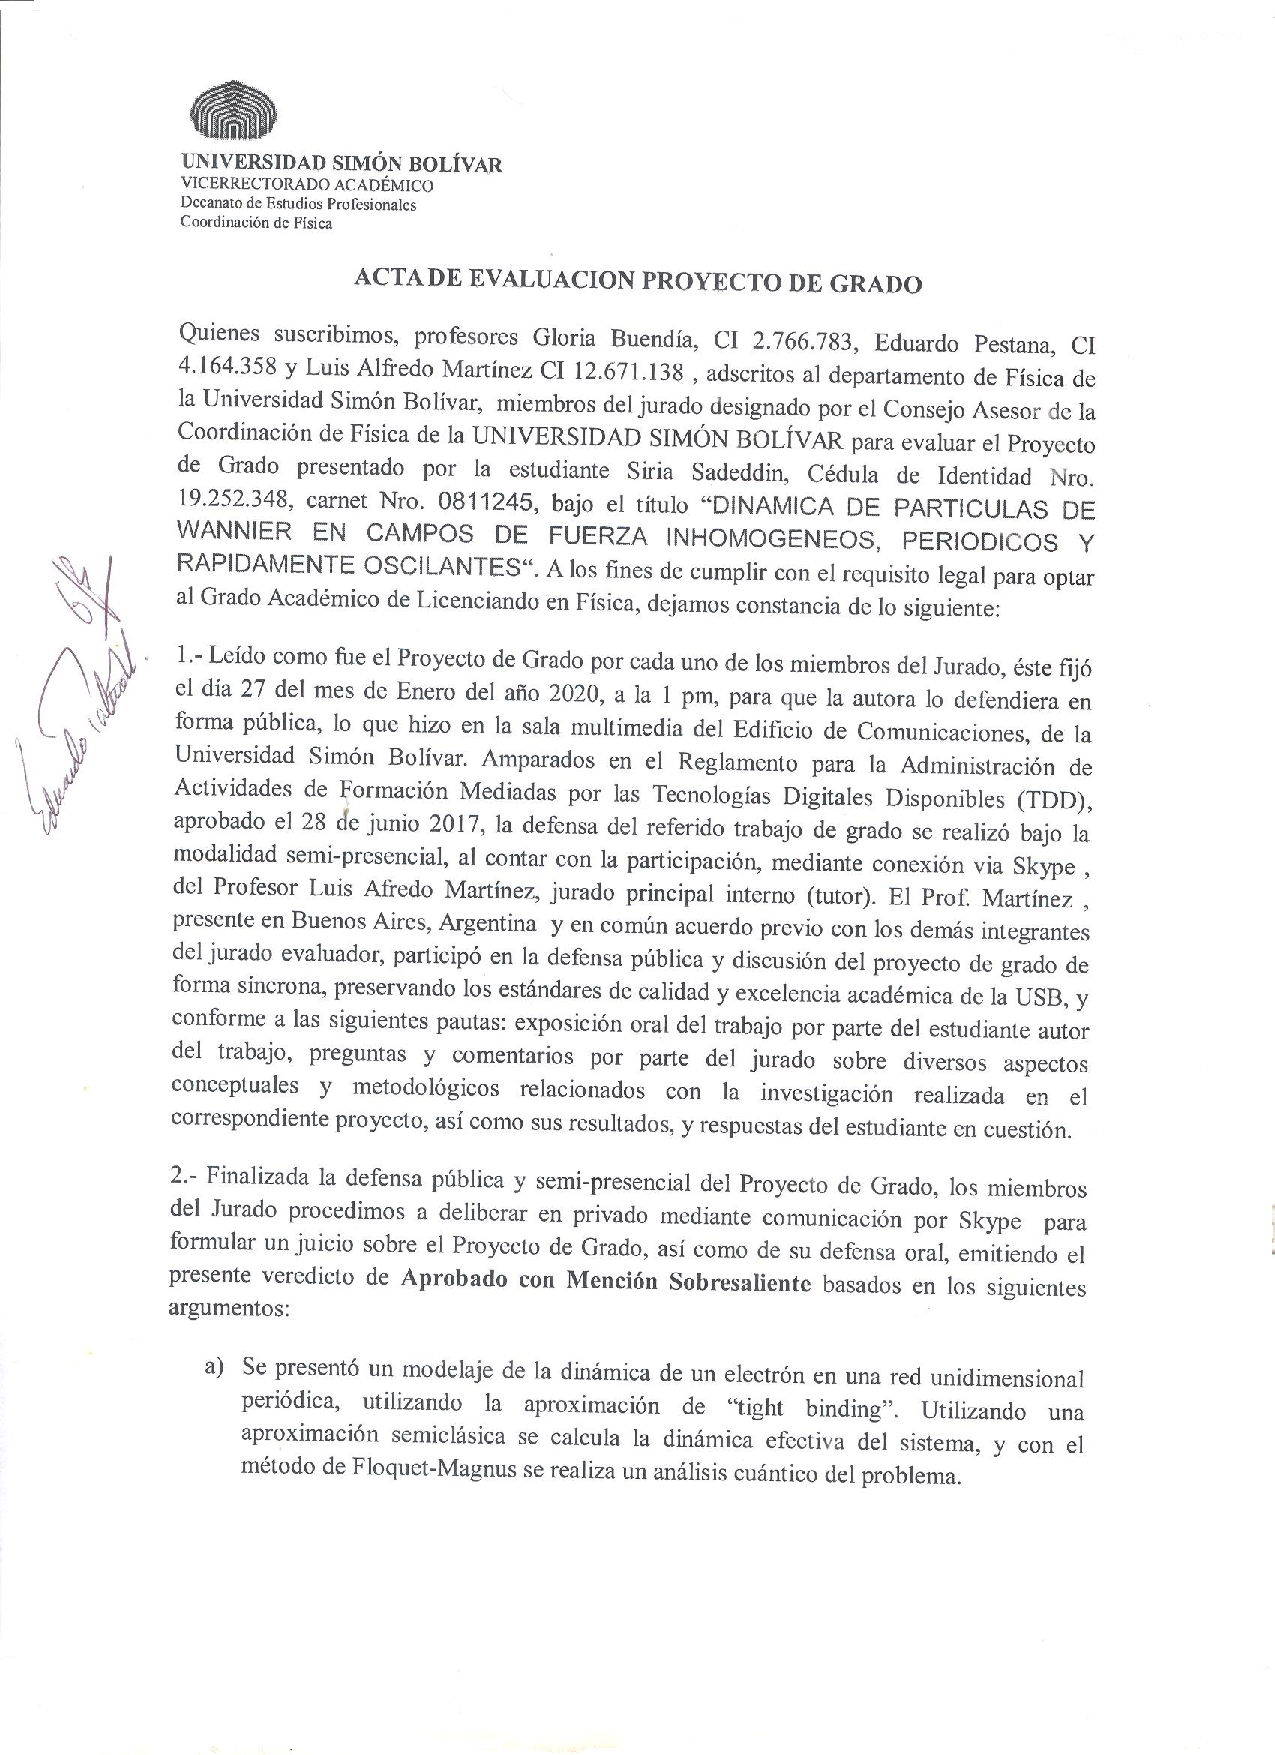
\includegraphics[width=1\columnwidth]{imagenes/ActadefensaSiria1.pdf}
\end{figure}

%\newpage
%\pagestyle{empty}
\begin{figure}
    \centering
    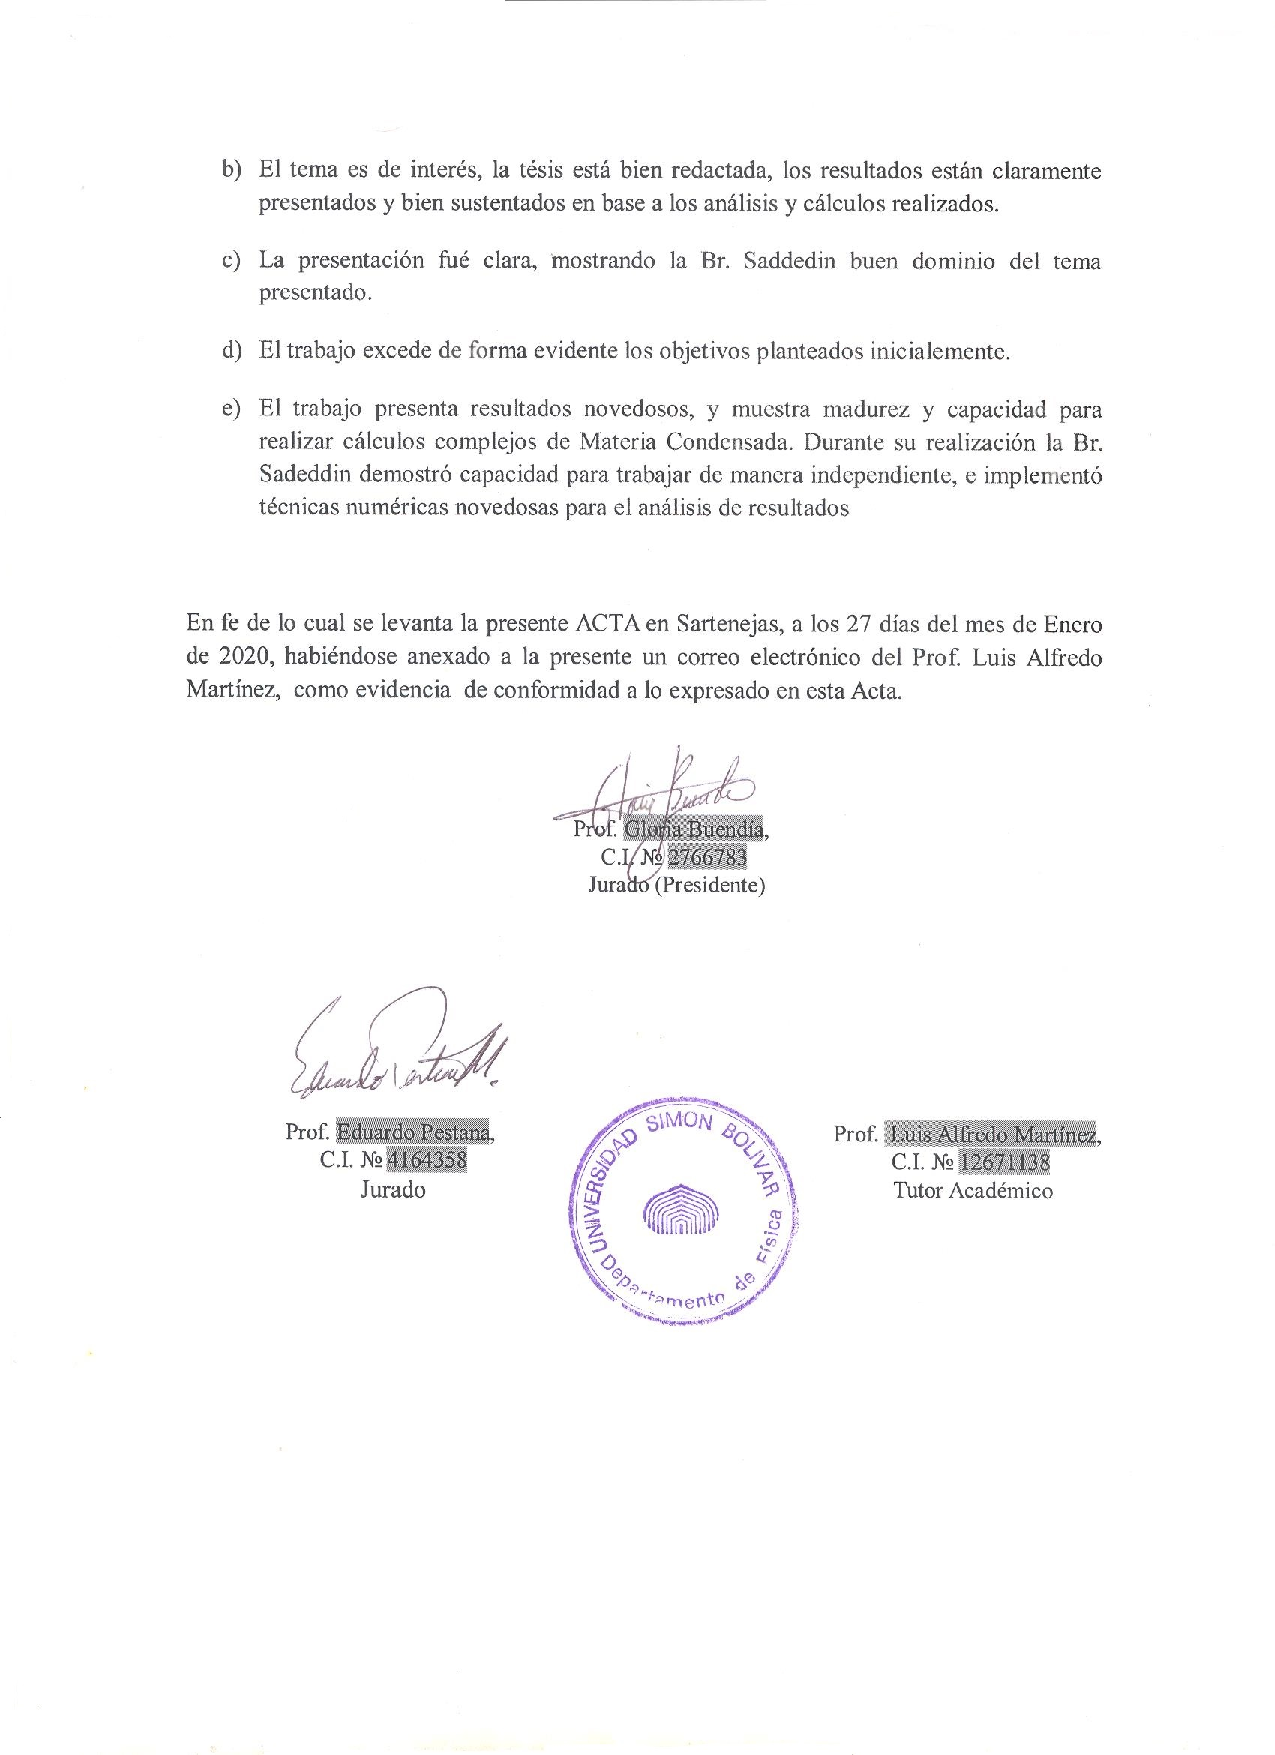
\includegraphics[width=1\columnwidth]{imagenes/ActadefensaSiria2.pdf}
\end{figure}


%\newpage
%\pagestyle{empty}

\begin{figure}
    \centering
    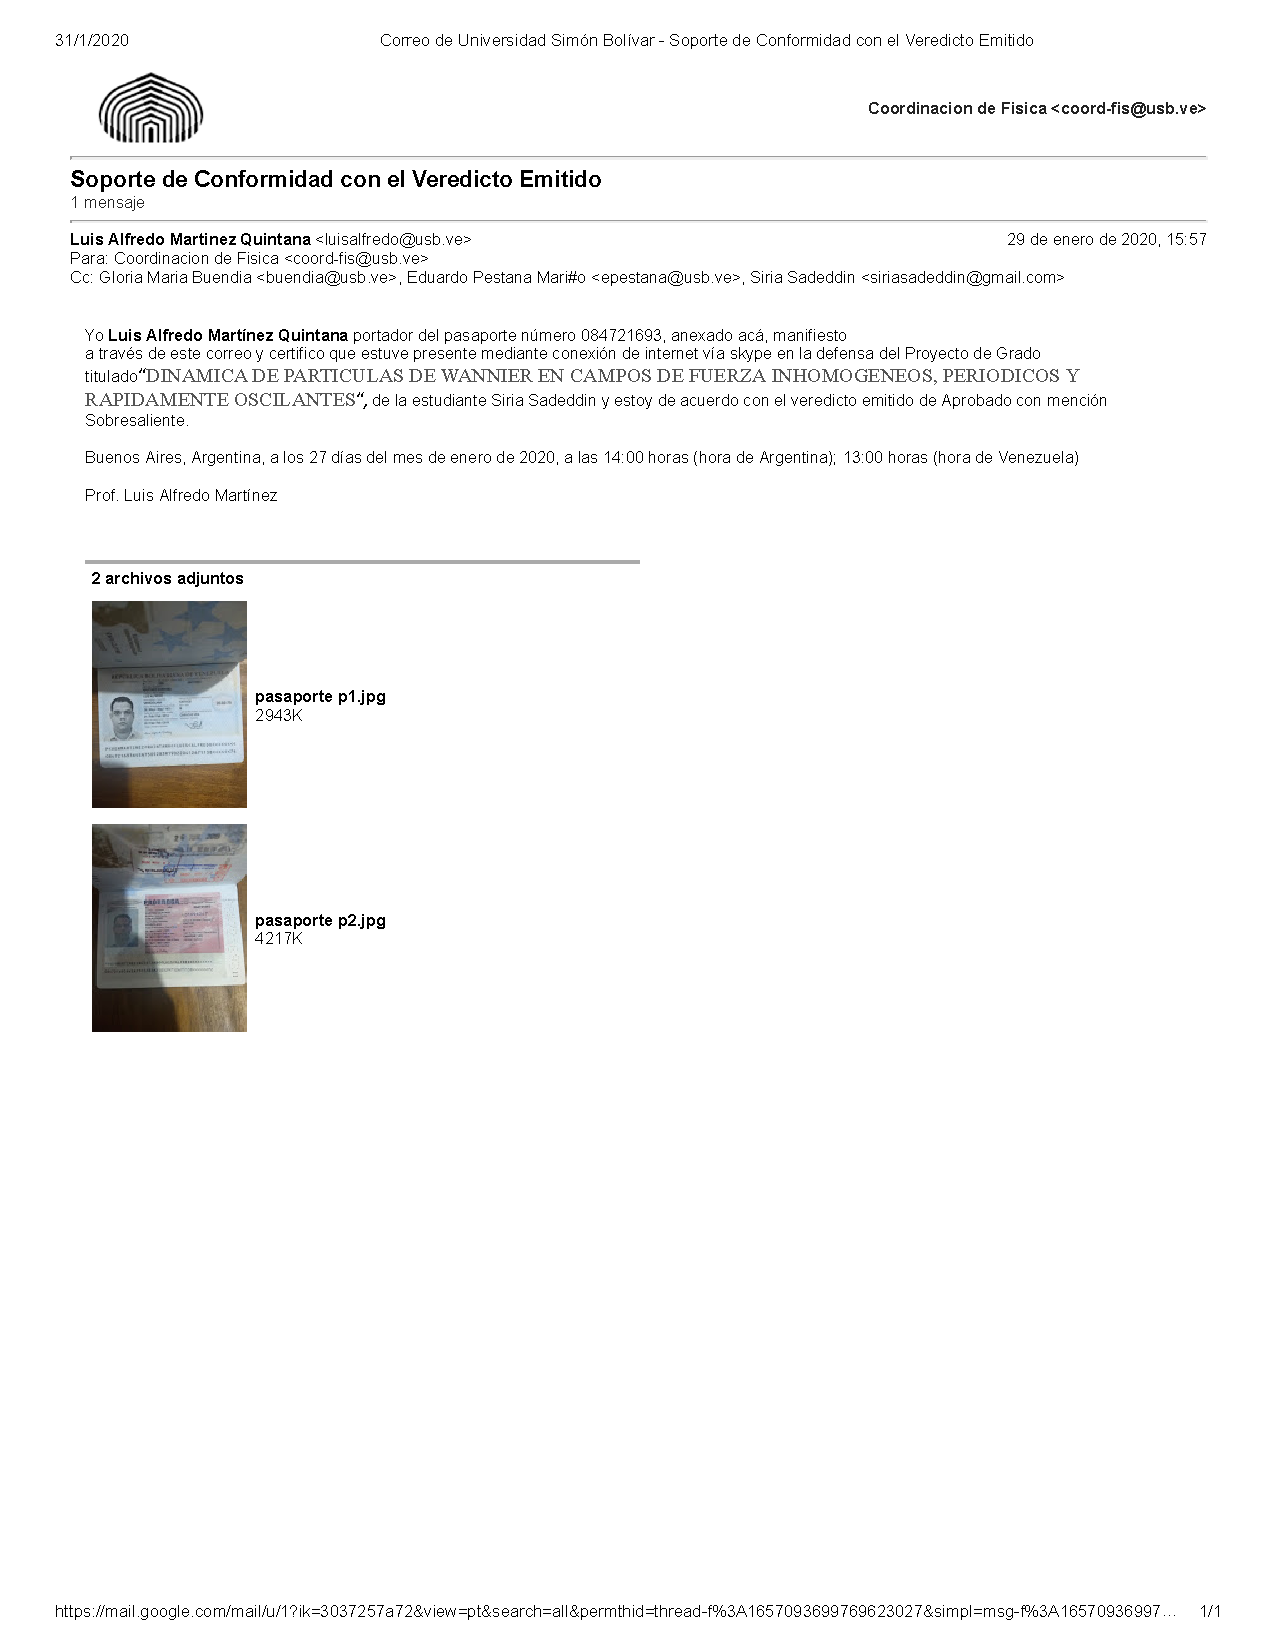
\includegraphics[width=1\columnwidth]{imagenes/SoportedeConformidadconelVeredictoEmitido.pdf}
\end{figure}

\frontmatter
\begin{resumen}
\setcounter{page}{7}

Se utiliza la aproximación de \textit{Tight Binding} para modelar la dinámica de un electrón en una 
red unidimensional, perfectamente periódica, homonuclear, sin impurezas, sin considerar  
transiciones de banda. El estudio se lleva a dos niveles, en primer lugar, semiclásico 
obteniendo la dinámica efectiva lenta del sistema sistema. A nivel cuántico, el estudio del sistema se lleva a cabo utilizando el método de Floquet-Magnus poniéndole en práctica a través de una técnica de cómputo simbólico implementada en Mathematica. Se estudia la dinámica del electrón en presencia de una perturbación lineal dependiente del tiempo, y se encuentra que el electrón experimenta deslocalización tanto en el caso semiclásico como en el cuántico, se observa la presencia del fenómeno de \textit{Band Narrowing} para ciertos valores de la frecuencia del potencial aplicado. En el caso no lineal se halla un comportamiento acotado del electrón, con presencia del fenómeno de localización dinámica. 
\vfill
\textbf{Palabras clave:} Electrón en una red, dinámicas rápida y lenta de Kapitza, Floquet-Magnus.
\end{resumen}
\chapter*{Dedicatoria}

A mi madre y padre.


\chapter*{Agradecimientos}

A la Universidad Simón Bolívar y su comunidad, a todos mis profesores, en especial a mi tutor Luís Alfredo Martínez, quien me introdujo en el campo de la Física del Estado Sólido y que me acompañó, personal y académicamente, en la realización de este proyecto. Al profesor Mario, quien no me dejó rendirme, y a mi Mamá quien nunca perdió la fe en mi. 


\tableofcontents
\listoffigures
\useacronyms
%\chapter*{Notaci\'on matem\'atica}
\begin{tabular}{ll}
$\mathbb{R}$ & Conjunto de n\'umeros reales\\
$M_{m,n}$ & Espacio de las matrices de tama\~no $m$ por $n$ con entradas reales\\
$\mathcal{L}$ & Operador de Laplace\\
$\emptyset$ & Conjunto vac\'io
\end{tabular}

\mainmatter
\chapter*{Introducción}

En un sólido cristalino los átomos se distribuyen de forma espacialmente regular constituyendo una red  periódica. Los electrones en la red pueden clasificarse en dos categorías enteramente diferenciadas: aquellos que están fijos a los orbitales internos de los átomos de la red; y aquellos que, por encontrarse en los orbitales más externos, pueden desligarse de dichos orbitales, y que forman lo que se conoce como estructura de bandas. 

Como un ejemplo de un fenómeno físico, de gran interés asociado a estructura de la red, puede comentarse que la conductividad eléctrica de un sólido está determinada por la respuesta de los electrones móviles de la red a los campos eléctricos externos \cite{kittel}. 

\begin{figure}[h]
    \centering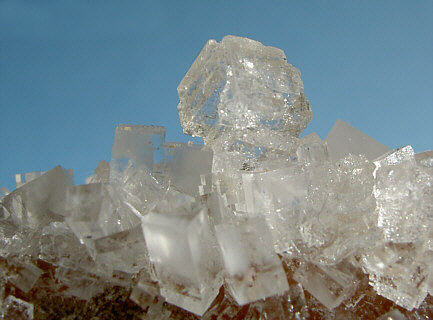
\includegraphics[scale=0.5]{./imagenes/NA-CL-Halit-Kristalle.jpg}
    \caption{Cristales de Halita (sal).}
    \label{fig:NACL_1}
\end{figure}

\begin{figure}[h]
    \centering
    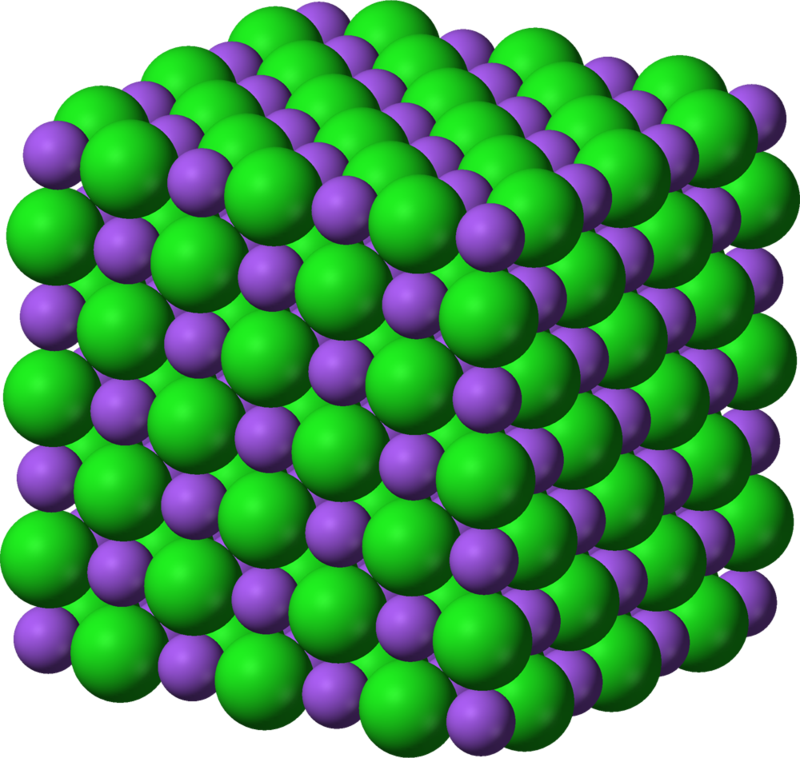
\includegraphics[scale=0.2]{./imagenes/NA-CL-Sodium-chloride-3D-ionic.png}
    \caption{Los átomos de sodio y cloro en su ordenamiento espacial}
    \label{fig:NACL_2}
\end{figure}


El problema de movilidad de los electrones en el sólido es, en principio, un problema de muchos cuerpos \cite{Fetter} \cite{kit_esteroides} . La dinámica de los electrones inmersos en la red debe tomar en cuenta no solo la interacción de los electrones con el potencial de los iones, sino también las interacciones electrón-electrón. El Hamiltoniano del i-ésimo electrón móvil de la red es: 

\begin{equation}
\mathbf{H}=\mathbf{T}_i+\sum_{j\neq{}i}\,V(r_{ij})+\sum_{j}\,U(r_{ij})\,,
\end{equation}
donde $\mathbf{T}_i$ es el operador de energía cinética del electrón, $V(r_{ij})$ el potencial de interacción entre el i-ésimo y el j-ésimo electrón y $U(r_{ij})$ el potencial de interacción con el j-ésimo núcleo en la red \cite{Fetter}. El tratamiento de la teoría en estos términos es sumamente complejo, y es por ello que se recurre a aproximaciones que han resultado sumamente exitosas.

En la aproximación de un solo electrón, todas las interacciones sobre este se representan por un solo potencial efectivo $U(\mathbf{r})$, cuando se pretende modelar un cristal perfectamente periódico el potencial efectivo resulta ser periódico \cite{ashc}. 
En términos cualitativos, se espera que, en el caso unidimensional homonuclear, de interés para este trabajo, el potencial cristalino típico tenga la forma que se muestra en la figura 
\ref{fig:periodic_potential}.
\begin{figure}[h]
    \centering
    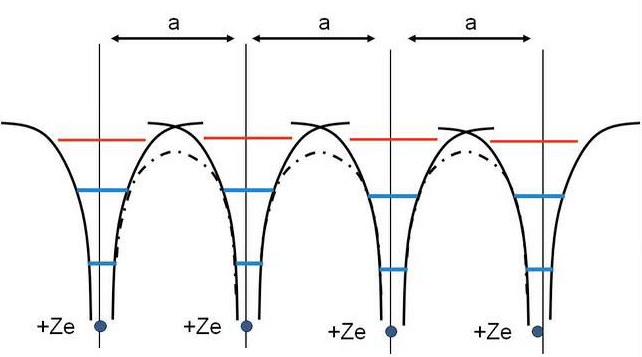
\includegraphics[scale=.5]{./imagenes/Periodic_Potential_1.png}
    \caption{Potencial periódico unidimensional}
    \label{fig:periodic_potential}
\end{figure}

La dinámica de electrones en redes periódicas fue extensamente estudiada por Bloch y Floquet, debido a esta razón histórica, los electrones en la red se llaman electrones de Bloch.

Expresado en términos modernos, el resultado fundamental de Bloch se expresa diciendo que la función de onda electrónica en una red periódica, porta una representación del grupo de traslaciones, es decir,
\begin{equation}
    \psi(x)=e^{ikx}\,u(x)\,,
\end{equation}
donde el número de onda ($k=2\pi/a$) se escoge dentro de la primera zona de Brillouin y $u$ es una función periódica de período $a$.

Otra de las aproximaciones que se utiliza, es la denominada aproximación de \textit{Tight Binding} \cite{ashc}, relacionada con el método de combinaciones lineales de orbitales atómicos que se utiliza ampliamente en química computacional, en particular en los denominados cálculos {\it{ab initio}}. El método consiste en utilizar una base del espacio de estados (lo que no implica resolver las ecuaciones del problema) para estudiar la estructura de bandas. El método de enlace fuerte lleva a una expresión altamente no lineal para la energía cinética del electrón en la red (relación de dispersión) $E=E(k)$ que constituye uno de los objetos fundamentales de este trabajo.

El fenómeno de \textit{Localización Dinámica} fue sugerido por el trabajo de Dunlap y  Kenkre en 1986 \cite{Dunlap}. Cuando un electrón en una red de \textit{Tight Binding} es sometido a un potencial eléctrico sinusoidal su posición inicial será restaurada en periodos del potencial aplicado. También se encuentra que el desplazamiento cuadrático promedio del electrón estará acotado y tendrá forma sinusoidal. Cuando el electrón presenta este comportamiento en las condiciones expuestas se dice que presenta localización dinámica. Para poder observar las oscilaciones en localización dinámica se debe cumplir la condición $\omega\tau>1$,donde $\tau$ es el tiempo libre medio del electrón. Para este proyecto de grado, se quiere estudiar el comportamiento dinámico de la partícula cuando el campo  eléctrico aplicado es inhomogéneo.

En la última década del siglo pasado, se hizo posible obtener cristales cuya distancia entre planos es del orden de $10$ \AA, cuando la distancia usual es de aproximadamente $1$ \AA$\,$   \cite{wannier2}, adicionalmente, ha sido posible disminuir de manera muy importante la cantidad de impurezas. En estos cristales, el tiempo de tránsito medio del electrón (antes de experimentar una dispersión) es mucho más largo que en un cristal convencional. Como consecuencia de estos avances técnicos, se ha hecho posible observar fenómenos que antes permanecían ocultos a la detección, como  por ejemplo, las oscilaciones de Bloch. Esto ha revivido el interés por los estudios teóricos de estos hechos lo que, sin duda, es una importante justificación para este trabajo. 

Matínez et al.\cite{mart2014} presentan un estudio semiclásico del movimiento de un electrón en una red cristalina, cuando sobre este actúa un potencial no homogéneo rápidamente oscilante, obteniendo una fórmula para el hamiltoniano efectivo de la dinámica lenta del sistema. En el 2017, Martínez y colaboradores retoman el estudio del mismo tipo de sistemas llevando el análisis a una formulación cuántica completa  \cite{martinez2017}

El objetivo general de este trabajo consiste en modelar la dinámica de un electrón en la red, cuando sobre él actúan campos externos inhomogéneos y rápidamente oscilantes; utilizando como método de estudio el modelo de \textit{Tight Binding}. 

En particular, se pretende modelar la dinámica del electrón en una red unidimensional, perfectamente periódica, homonuclear, sin impurezas, restringiendo al electrón a mantenerse dentro de una sola banda, es decir, sin considerar transiciones de banda. 

En vista de que el sustrato en el que se encuentra el electrón es una red (potencial periódico), se utilizan la teoría de Floquet y el teorema de Bloch. En el trabajo se buscan potenciales efectivos y se hacen tanto estudios semiclásicos como cuánticos logrando reproducir los resultados de Martínez et al. (2014) \cite{mart2014} y  Martínez et al. (2017), y estudiando la dinámica de partículas en campos no homogéneos.

En el enfoque semiclásico se utiliza el método de Kapitza para partículas clásicas con perturbaciones externas rápidamente oscilantes, y se aplica al electrón en la red. Kapitza estudió partículas clásicas en presencia de campos rápidamente oscilantes, concluyendo que el sistema se puede modelar separando los movimientos de la partícula en uno rápido y otro lento. Y, a partir de allí encuentra el potencial efectivo.

Se obtiene la forma de la aceleración efectiva del electrón dentro del cristal, y, probando perturbaciones específicas se puede hallar el potencial efectivo y así hacer un modelo para la dinámica del electrón bajo la influencia de  cualquier potencial externo, rápidamente oscilante o no. 

En interesante hacer el estudio cuántico por su exactitud. En particular, se utilizara un enfoque perturbativo, basado en los trabajos de Floquet- Magnus y el método de Maricq.  Se estudia el efecto de los potenciales externos sobre un electrón en una red de enlace fuerte. Este es un método aproximado, la expansión de Floquet-Magnus aproxima el Hamiltoniano efectivo del electrón en la red en presencia de la perturbación. Esta aproximación se hace hasta cierto orden, en este caso se utiliza una aproximación hasta el orden de $1/\omega^2$. Términos de correcciones superiores no se toman en cuenta. 

En este trabajo especial de grado, se este quieren hallar las soluciones a la ecuación de Schrödinger del electrón en la red de \textit{Tight Binding} bajo dicho potencial externo. De esta manera es posible obtener las autoenergías del electrón bajo las condiciones mencionadas y hallar las autofunciones de la ecuación de Schrödinger, y así estudiar la auto dinámica del electrón en presencia del potencial externo. Para hacer esto se utilizan las ecuaciones diferenciales de Hill, en el caso particular de estas, las ecuaciones de Mathieu.  Se encuentra que el Hamiltoniano efectivo para el electrón en una red de enlace fuerte, bajo el efecto de un potencial externo, tiene forma similar a las ecuaciones de Hill.

En cada capítulo se desarrolla un tema de interés físico y se introducen algunos de los métodos matemáticos que permiten derivar los resultados del capítulo.

En el capítulo I se introduce la teoría de bandas de los sólidos. La teoría de bandas permite comprender la movilidad de los electrones en los solidos. Se presenta la Teoría de Floquet, esta teoría permite hallar soluciones a las ecuaciones diferenciales de coeficientes periódicos, valiosa para estudiar la dinámica del electrón en la red periódica cristalina. Se estudia teorema de Bloch cuyos resultados permiten conocer la forma de las funciones de onda asociadas al electrón en la red. Finalmente se estudian las ecuaciones de Hill cuyas soluciones serán importantes a la hora de estudiar la dinámica del electrón en la red de enlace fuerte. Se presenta la teoría de enlace fuerte, como enfoque principal que se usará para el modelado de los solidos a estudiar en este trabajo de grado. 

En el capítulo II se da una discusión del método de Kapitza para el cálculo del potencial efectivo clásico para una partícula sometida a un campo externo rápidamente oscilante. Se estudia el método semiclásico en física del estado solido y las condiciones para su adecuada aplicación. Se explica además como caso de uso el fenómeno de las oscilaciones de Bloch, como consecuencia del efecto de un potencial independiente del tiempo y homogéneo sobre el electrón en la red.

En el capítulo III se presenta el método de Floquet-Magnus para el cálculo de Hamiltonianos efectivos cuánticos del electrón, bajo el efecto de campos externos oscilantes.

En el capítulo IV se hace uso del método de Kapitza para el estudio de la dinámica semiclásica de un electrón en la red de enlace fuerte en presencia de potenciales rápidamente oscilantes. Se obtiene un resultado original de este proyecto de grado que permite saber el potencial efectivo experimentado por el electrón en la condiciones particulares del estudio. Con ayuda del resultado obtenido se estudia la dinámica del electrón para varios casos.

Finalmente, en el capítulo V se aplica el método de Floquet-Magnus al cálculo de Hamiltonianos efectivos cuánticos y se resuelven algunos casos particulares.  


\chapter{El electrón en la red periódica}

\section{Teoría de Bandas}\label{cap:1}
El problema de la movilidad de los electrones en los sólidos y la existencia de conductores y aislantes seguía siendo un misterio a principios del siglo XX. El modelo de Drude, propuesto en el año 1900, modela los electrones en el sólido como un gas ideal de partículas clásicas, que se mueven aleatoriamente en linea recta e interactúan a través de colisiones con los núcleos inmóviles de los átomos. Dos cantidades físicas son importantes en este modelo: el tiempo entre colisiones $\tau$ y el camino libre medio entre colisiones $l$. El modelo de Drude fue exitoso en explicar el efecto Hall, la conductividad térmica y eléctrica; pero no explica por qué algunos sólidos presentan conductividad eléctrica y otros no \cite{kittel}.

Para entender la conductividad de los distintos materiales, es necesario tomar en consideración la naturaleza cuántica y la estructura interna periódica cristalina del sólido. El descubrimiento de la teoría cuántica y el principio de exclusión de Pauli permitieron que Sommerfield resolviera el problema del calor específico, el cual no había sido resuelto por Drude. El modelo de Somerfield estudia, de forma muy similar a Drude, al gas de electrones, pero tomando en cuenta la estadística de Fermí-Dirac en sus cálculos. Ambos modelos, llamados en conjunto \textit{Modelo de Electrones Libres} permiten tener una idea acertada sobre la capacidad térmica, la conductividad térmica, la conductividad eléctrica, la susceptibilidad magnética y la electrodinámica en los metales, pero no resuelve el problema de la conducción en metales, semimetales, semiconductores y aislantes \cite{ashc}.

La Teoría de Bandas permite explicar la diferencia en la conductividad eléctrica de los conductores, semiconductores y aisladores \cite{valen}. El trabajo de Bloch sobre las funciones ondulatorias de electrones en la red cristalina y los casi simultáneos trabajos de Pierls y Bethe, abrieron el camino de la Teoría de Bandas. La alta conductividad no se relaciona directamente con un alto grado de movilidad de los electrones, pues estos necesitan encontrar estados libres en las bandas de energía; si tales estados no existen, el cristal será un aislante \cite{Kragh}.

En un átomo aislado, los electrones ocupan orbitales bien definidos de energía que están cuantizados. Cuando dos átomos idénticos se acercan para formar una molécula, las funciones de onda de los electrones que ocupan los mismos orbitales en cada uno de los átomos comienzan a interactuar. El principio de exclusión de Pauli, impide que existan dos electrones en el mismo estado cuántico compartiendo un mismo orbital, debido a esto, dichos orbitales experimentan una separación de los estados, separándose las energías y apareciendo dos nuevos estados discretos. En los sólidos, este mismo proceso ocurre en el orden de $10^{23}$ veces, ocasionando que la separación de los estados sea muy pequeña (del orden de $10^{-23}$ eV), esto crea un cuasicontínuo de niveles de energía que se denomina banda. En un cristal de $N$ sitios, si se toma en cuenta que por cada estado cuántico puede existir dos electrones con spin opuesto, se tendrá $2N$ estados permitidos para llenar la banda.

Para un electrón libre, la energía está dada en $k$:

\begin{equation}\label{eq:1.1}
    E_k=\frac{\hbar^2k^2}{2m}\,.
\end{equation}

En ausencia de cualquier interacción entre orbitales, los niveles de energía electrónicos están dados por una parábola en el espacio $k$. Esto se mantiene cierto incluso cuando se incluye un potencial periódico débil, excepto en la zona cercana a los \textit{Planos de Bragg}. En este modelo, llamado del \textit{Electrón casi libre}, la interacción del electrón con el potencial periódico de la red ocasiona una corrección de los niveles de energía del electrón libre cerca de los planos de Bragg. La energía se corrige dibujando otra parábola centrada en $k$, donde $k$ es el vector recíproco del cristal. La curva original se modifica, tal como se muestra en la figura \ref{fig:1.2} a. Esta representación de los niveles de energía se llama \textit{Esquema de zonas extendido} \cite{ashc}. La degeneración de los niveles electrónicos en los planos de Bragg ocasiona que las energías en las cercanías de los planos se separen. La energía del electrón en el modelo del \textit{Electrón casi libre} en dos dimensiones bajo el esquema de perturbación, resulta ser: 

\begin{equation}\label{eq:1.2}
    \mathcal{E}=\mathcal{E}^{K}_{0} \pm |U_K|
\end{equation}

Donde $\mathcal{E}^{K}_0$ es la energía en ausencia del potencial periódico, y $|U_K|$ el módulo de la componente de Fourier del potencial periódico en el el espacio recíproco.

\begin{figure}[H]
    \centering
    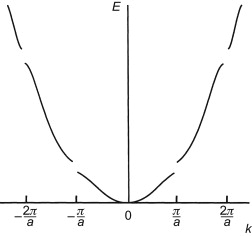
\includegraphics[scale=1]{imagenes/esquema_bandas.jpg}
    \caption{Esquema extendido de bandas, las discontinuidades de la parábola indican bandas prohibidas.}
    \label{fig:1.1}
\end{figure}


 El espacio que se forma debido a la discontinuidad en la curva corresponde a energías prohibidas. Estas regiones se denominan \textit{Bandas prohibidas}  y ningún electrón puede ocupar estos niveles. Como se ha visto, estas  resultan de la interacción de las ondas de electrones de conducción con los núcleos de iones del cristal \cite{kittel}. La forma en que los electrones del solido llenan las bandas permitidas determina si este será un conductor, semiconductor o aislador. Se denomina banda de valencia a la ultima banda totalmente llena del solido,  la banda vacía, inmediatamente por encima de la banda de valencia, se denomina \textit{Banda de Conducción} \cite{valen}.

En la aproximación de \textit{Tight Binding} (sección \ref{cap:5}), el potencial de la red es comparable con la energía del electrón y las funciones de onda de los electrones vecinos se superponen parcialmente. Tomando en consideración solo los primeros vecinos, se obtiene la relación de dispersión:

\begin{equation}\label{eq:1.3}
    \mathcal{E}=\mathcal{E}_0-2A\cos(ak)
\end{equation}

Es evidente, partiendo de esta ecuación, que la energía estará acotada entre dos valores ($\mathcal{E}_0 \pm 2A$) formando las bandas permitidas en el sólido. 

Tanto la aproximación de \textit{Tight Binding}, como la aproximación de electrones casi libres, son útiles dependiendo del sólido a estudiar. El modelo de electrón casi libre es usado frecuentemente en metales, mientras que el modelo de enlace fuerte es bastante usado para semiconductores y aislantes. 
La forma en la que se llenan las bandas determina la conductividad del sólido, el cristal se comporta como un metal si una o más bandas están parcialmente llenas. El cristal es un semiconductor, o un semimetal, si hay bandas están ligeramente llenas o ligeramente vacías \cite{kittel}. A la temperatura de cero absoluto, los electrones llenan las bandas en orden ascendente a partir de su estado mas bajo, hasta una energía dada que se determina de acuerdo al número de estados disponibles, y el numero de electrones del cristal. Este último estado en llenarse es la energía de Fermi del cristal en el cero absoluto \cite{solidos}. En un cristal unidimensional algunas de las bandas permitidas están totalmente llenas, parcialmente llenas o totalmente vacías. Las bandas totalmente llenas o vacías no pueden contribuir a la corriente. En una banda totalmente llena no hay estados disponibles para que los electrones puedan ser excitados gradualmente, por lo que estos electrones se encuentran atrapados en la banda.

En un aislador, el número de electrones del cristal es suficiente para llenar completamente cierto número de bandas, pero la brecha prohibida entre la última banda llena y la primera vacía es tan ancha (alrededor de $15$ eV), que es prácticamente imposible excitar térmicamente un número importante de electrones hacia la banda vacía. Por lo tanto en un aislante solo hay bandas llenas o vacías, y no fluye ninguna corriente de electrones libres.

Si la brecha prohibida en este tipo de sólidos es lo suficientemente pequeña (alrededor de 1 eV), existe una probabilidad estadística apreciable de que los electrones puedan excitarse a estados de la banda vacía, permitiendo un flujo de corriente. A estos materiales se les llama semiconductores. 

\begin{figure}[H]
    \centering
    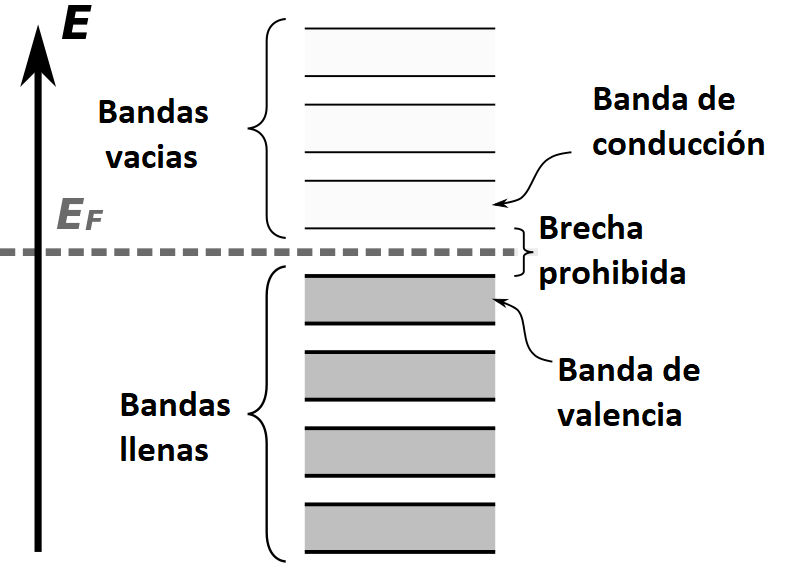
\includegraphics[scale=.5]{imagenes/Semiconductor_band_structure.png}
    \caption{Esquema de bandas para un semiconductor}
    \label{fig:1.2}
\end{figure}

Todo semiconductor tiende a volverse aislador a medida que se enfría el material acercándose al cero absoluto (a excepción de los superconductores) y un aislador puede comportarse como semiconductor si alcanza la temperatura suficiente. Sin embargo, esta situación es muchas veces imposible de obtener en la práctica, ya que el sólido se funde o evapora \cite{solidos}.



%%%%%%%%%%%%%%%%%%%%%%%%%%%%%%%%%%%%%%%%%%%%%%%%%%%%%

\section{Teoría de Floquet}\label{cap:2}

El objetivo de este capítulo consiste en establecer las bases generales del comportamiento de un electrón en una red cristalina unidimensional. Con este fin, se presenta la teoría de Floquet para la solución de ecuaciones diferenciales ordinarias de segundo orden con coeficientes periódicos.

El sobresaliente matemático Achile Marie Gaston Floquet (1847-1920) hizo grandes contribuciones en el campo de las matemáticas y análisis matemático.
En el campo de las ecuaciones diferenciales ordinarias, uno de sus desarrollos mas prominentes es su {\it{Teorema de Floquet}} (1883), que permite obtener una forma canónica para cada matriz fundamental de soluciones a los sistemas de ecuaciones diferenciales lineales periódicas \cite{mananga}. Adicionalmente, la Teoría de Floquet estudia las ecuaciones diferenciales ordinarias periódicas y sus soluciones, así como su estabilidad. 
La Teoría de Floquet es de interés particular cuando se quiere investigar sistemas dinámicos, por ejemplo, a las ecuaciones de Mathieu y las ecuaciones diferenciales de Hill, usadas para aproximar el movimiento lunar.

\subsubsection{Teoría general de Floquet}

El Teorema de Floquet es equivalente al Teorema de Bloch en Física de Materia Condensada \cite{mananga}. Considérese una ecuación diferencial de segundo orden de la forma:

\begin{equation}\label{eq:2.1}
    a_0(x)f''(x)+a_1(x)f'(x)+a_2(x)f(x)=0
\end{equation}

Donde los coeficientes complejos $a_r(x)$ son funciones periódicas y continuas a trozos que comparten exactamente el mismo periodo real: $a>0$ \cite{floquet}:

\begin{equation}\label{eq:2.2}
    a_r(x+a)=a_r(x)\,,\quad{}0\leq{}r\leq{}2\,,
\end{equation}

$a_0(x)$ no se anula en ningún punto de su dominio, evitando así singularidades en la ecuación diferencial. Se sigue que, si $\psi(x)$ es una solución a la ecuación diferencial, entonces $\psi(x+a)$ será también solución, sin decir con esto que $\psi(x)$ es periódica, o que $\psi(x)$ y $\psi(x+a)$ sean la misma función \cite{floquet}. Sin embargo $\psi$ tiene una propiedad, que se expone en el teorema \ref{teo:2.1}.\\

\begin{teo}\label{teo:2.1}

Existe una constante no nula $\rho$ y una solución no trivial $\psi(x)$ de \ref{eq:2.1} tal que se cumple la ecuación \ref{eq:2.3}. \cite{floquet} (apéndice \ref{apendice:A.1}).

\begin{equation}\label{eq:2.3}
    \psi(x+a)=\rho\, \psi(x)
\end{equation}

\end{teo}

\begin{teo}\label{teo:2.2}
Existen soluciones linealmente independientes de \ref{eq:2.1}, $\psi_1(x)$ y $\psi_2(x)$ tales que:

\begin{equation}\label{eq:2.4}
    \psi_1(x)=e^{m_1x}p_1(x)
\end{equation}

\begin{equation}\label{eq:2.5}
    \psi_2(x)=e^{m_2x}p_2(x)
\end{equation}

Donde $m_1$ y $m_2$ son constantes, no necesariamente distintas, y $p_1(x)$ y $p_2(x)$ son periódicas con periodo $a$ \cite{floquet} \ref{apendice:A}. Y en general, existen $k$ soluciones a \ref{eq:2.1} tales que: 

\begin{equation}\label{eq:2.6}
    \psi_k(x)=p_k(x)\,{}e^{m_kx}
\end{equation}

\end{teo}


\subsubsection{Teoría de Floquet en sistemas lineales}

La teoría de Floquet puede extenderse a sistemas lineales, de la siguiente manera:

\begin{equation}\label{eq:2.7}
    f'(x)=C(x)f(x)
\end{equation}

Donde $C(x)$ es una matriz de variable compleja, suave a trozos y de tamaño $n \times n$ tal que: 

\begin{equation}\label{eq:2.8}
    C(x+a)=C(x)
\end{equation}

Donde $a$ es una constante no nula. Denotaremos con minúsculas los vectores de $n$ componentes, y con mayúsculas a las matrices.

\begin{teo}\label{teo:2.3}
Existe una constante no nula $\rho$, y una solución no trivial $\psi(x)$ a \ref{eq:2.7} tal que: 

\begin{equation}\label{eq:2.9}
    \psi(x+a)=\rho \psi(x)
\end{equation}

La prueba a este, es análoga al teorema \ref{teo:2.1} \cite{floquet} \ref{apendice:A}.\\ 
\end{teo}

\begin{teo}\label{teo:2.4}
Existen $n$ soluciones de \ref{eq:2.7} linealmente independientes $\psi_k(x)$ tales que:

\begin{equation}\label{eq:2.10}
    \psi_k(x)=e^{im_kx}p_k(x)
\end{equation}

Sea $\Psi(x)$ la matriz fundamental de \ref{eq:2.7}, entonces se cumple la siguiente igualdad:

\begin{equation}\label{eq:2.11}
    \Psi(x+a)=\Psi(x)B
\end{equation}
\cite{floquet} \ref{apendice:A}
\end{teo}

Estos resultados pueden ser expresados en términos de matrices. Como $B$ es una matriz no singular,existe una matriz $M$ tal que:

\begin{equation}\label{eq:2.12}
    B=e^{Ma}
\end{equation}

Por lo que se define un $P(x)$ análogo a \ref{eq:2.6} y se definen las soluciones al sistema de ecuaciones lineales en la forma \ref{eq:2.13}; donde $P(x)$ es periódico, de periodo $a$ \cite{floquet}:

\begin{equation}\label{eq:2.13}
    \Psi(x)=P(x)e^{Mx}, \     P(x)=P(x+a)
\end{equation}

%%%%%%%%%%%%%%%%%%%%%%%%%%%%%%%%%%%%%%%%%%%%%%%


\section{Teorema de Bloch}\label{cap:3}

En 1928, Felix Bloch, descubrió que el momento cristalino es una cantidad conservada, sin importar lo poderoso que sea el potencial periódico. Este descubrimiento se conoce como el Teorema de Bloch, y establece que un electrón en un potencial periódico tiene autoestados de la siguiente forma \cite{oxford}:

\begin{equation}\label{eq:3.1}
\Psi_{k}(x)=e^{ikx}u_{k}(x)
\end{equation}

Donde $u(k)$ es periódico en la celda unitaria y k (el momento cristalino) puede elegirse dentro de la primera zona de Brillouin \cite{oxford}. Las funciones propias de la ecuación de ondas para un potencial periódico son el producto de una onda plana $e^{ikx}$ por una función $u_k(x)$ que posee la periodicidad de la red cristalina \cite{kittel}.

El teorema de Bloch propone una forma para las funciones de onda asociadas a un electrón en presencia de un potencial perfectamente periódico. Sea una ecuación diferencial que tiene la forma de la siguiente ecuación \cite{solidos}:

\begin{equation}\label{eq:3.2}
    \frac{d^2\Psi(x)}{dx^2}+V(x)\Psi(x)=0
\end{equation}

Donde $V(x)$ es una función periódica con periodo del parámetro de red $a$, que corresponde a la distancia que existe entre los iones del cristal, en este caso unidimensional (ver figura \ref{fig:3.1}).

\begin{figure}[H]
    \centering
    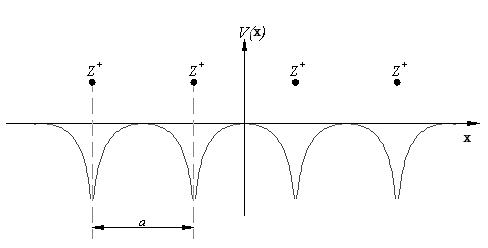
\includegraphics{imagenes/potencial-red.png}
    \caption{Potencial periódico de la red, imagen referencial tomada de http://en.wikipedia.org en.wikipedia}
    \label{fig:3.1}
\end{figure}

Tomando en cuenta el teorema \ref{teo:2.1}, se pueden definir soluciones $\Psi(x)$ para la ecuación \ref{eq:3.2}, que cumplen con las condiciones siguientes:

\begin{equation}\label{eq:3.3}
    \Psi(x+a)=\rho\,\Psi(x),\qquad{} \rho=e^{ika}
\end{equation}

Se sabe por el teorema \ref{teo:2.1} que $\Psi(x)$ puede escribirse como sigue, donde se define un $u_k(x)$ periódico, de periodo $a$:  

\begin{equation}\label{eq:3.4}
    \Psi_k(x)= e^{ikx}u_k(x)
\end{equation}

\begin{equation}\label{eq:3.5}
    u_{k} (x+a) =u(x)_{k}
\end{equation}

La ecuación \ref{eq:3.4} son las llamadas \textit{Funciones de Bloch}. Como se puede notar, se trata de ondas planas, con vector de propagación $k$ y que están moduladas por funciones periódicas $u(x)_k$ (ver figura \ref{fig:3.2}).

\begin{figure}[H]
    \centering
    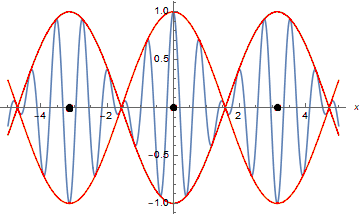
\includegraphics[scale=.7]{imagenes/Bloch_function.png}
    \caption{Funciones de Bloch, dibujo referencial}
    \label{fig:3.2}
\end{figure}

Se concluye entonces que la red tiene el efecto de deslocalizar el paquete de onda del electrón, de tal manera que ya no es posible determinar la posición del electrón en un punto específico del sólido. 
Ahora, se aplican condiciones de frontera periódicas de Born–von Karman sobre $\Psi(x)$ (ecuación \ref{eq:3.6}). Estas son condiciones de frontera que permiten establecer una continuidad en el solido finito. Se supone que la red está compuesta por N sitios, y que el valor de la función en la primera posición es igual a la ultima posición, esto se conoce también como red de anillo \cite{solidos}. Las condiciones Born–von Karman implican que $e^{ikNa}=1$. De esta expresión se obtiene que $k$ tiene valores bien definidos dados por la ecuación \ref{eq:3.7}:

\begin{equation}\label{eq:3.6}
    \Psi_k(x+Na)=e^{ikNa}\Psi_k(x)=\Psi_k(x)
\end{equation}

\begin{equation}\label{eq:3.7}
k_n=\frac{2\pi n}{Na}, \ n={0,1,2,...,N}
\end{equation}

De este resultado se obtiene que el electrón puede tener tantos estados posibles de $k$ como sitios posea la red.

%%%%%%%%%%%%%%%%%%%%%%%%%%%%%%%%%%%%%%%%%%%%%%%%%%%%%

\section{Ecuaciones de Hill}\label{cap:4}

Las ecuaciones de Hill pertenecen a la clase de ecuaciones diferenciales lineales homogéneas de segundo orden con coeficientes reales periódicos. A pesar de que estas ecuaciones fueron investigadas desde mucho antes de la publicación sobre el movimiento lunar de Hill en 1877 \cite{moon}, se les ha dado ese nombre por sus importantes contribuciones a la teoría. Las ecuaciones de Hill tienen muchas aplicaciones en problemas de ingeniería y física, en especial para mecánica, astronomía, teoría de circuitos eléctricos, y la conductividad en metales. 
Un resultado importante de la teoría de Hill es que esta revela la ocurrencia de un fenómeno sorprendente: si una fuerza que varía periódicamente en el tiempo actúa sobre una masa, de tal manera que la fuerza tiende a mover la masa alrededor de una posición de equilibrio, uno puede esperar que la masa se mantenga confinada a una vecindad de la posición de equilibrio. En particular, entre mayor sea la fuerza uno esperaría que esta fuese mas eficiente en este propósito, sin embargo este no es el caso. Un incremento en la fuerza puede causar que la partícula oscile con mayor amplitud cada vez. La teoría de intervalos de estabilidad en las ecuaciones de Hill provee una descripción precisa de este fenómeno.
La ecuación diferencial de Hill tiene la forma general: 

\begin{equation}\label{eq:4.1}
    \frac{\partial^2}{\partial t^2}y+f(t)y=0
\end{equation}

Donde $f(t)$ es una función periódica de periodo $a$, debido a esto, se puede escribir la ecuación en series de Fourier como sigue: 

\begin{equation}\label{eq:4.2}
   \frac{\partial^2}{\partial t^2}y+\left(\theta_0+2\sum^{\infty}_{n=1}\theta_n\cos(2nt)+2\sum^{\infty}_{n=1}\phi_n\sin(2nt)\right)y=0
\end{equation}

Un caso especial para las ecuaciones de Hill son las ecuaciones de Mathieu. En este caso $f(t)$ es una función par y $n=1$.

Émile Léonard Mathieu (1835-1890) fue un matemático francés, cuyas contribuciones más importantes están en la teoría de grupos y la física matemática. Su nombre aparece en las \textit{Ecuaciones de Mathieu}, \textit{Grupos de Mathieu} y la \textit{Transformación de Mathieu}. Su descubrimiento sobre las \textit{Ecuaciones de Mathieu} se produjo mientras estudiaba las vibraciones de la membrana elíptica. La expresión general de la ecuación de Mathieu tiene la siguiente forma:

\begin{equation}\label{eq:4.3}
    \frac{\partial^2u}{\partial Z^2}+\left(\theta_0+2\theta_1\cos(2Z)\right)u=0
\end{equation}

Muchas propiedades de las \textit{Ecuaciones de Mathieu} se pueden deducir a partir de la \textit{Teoría de Floquet}. Aparecen en un gran número de contextos en ingeniería, física, y matemática aplicada. Tiene aplicaciones en el estudio de ecuaciones con geometría elíptica, y también se aplican a problemas dinámicos con fuerzas que son periódicas en el espacio o en el tiempo.
Las \textit{Funciones de Mathieu} juegan un papel importante en sistemas mecánico-cuánticos, en especial aquellos que incluyen potenciales periódicos, por ejemplo, el péndulo cuántico y las redes cristalinas. Se verá, mas adelante, que la ecuación de Schrödinger, que describe al electrón en la red de Enlace Fuerte y en presencia del potencial rápidamente oscilante, es una ecuación diferencial de Hill o de Mathieu. A continuación se describirá un método analítico para hallar las soluciones a esta ecuación diferencial.
En 1868, Mathieu halló que la \textit{serie periódica doble} es solución a la ecuación diferencial de Mathieu.

\begin{teo}{\textbf{Teorema de Floquet}}\label{teo:4.1}:
Debe ser posible encontrar dos soluciones diferentes de la forma $x=e^{i\lambda z}$ multiplicada por una serie de Laurent en $x^2$. Una serie de Laurent en $x^2$ es una serie de potencias enteras positivas y negativas de x, esto es, una
serie de Fourier en $2z$. Esta serie es periódica en $z$,con periodo $\pi$, y puede representar la función alrededor de los puntos singulares $x = 0$ y $x = \infty$. Escogemos entonces a la ecuación \ref{eq:4.4} como una solución \cite{Philip}:

\begin{equation}\label{eq:4.4}
    u=e^{i\lambda z}\sum^{\infty}_{n=-\infty} b_n e^{2inz}
\end{equation}

\end{teo}

La ecuación \ref{eq:4.4} es una solución a la ecuación de Mathieu, donde $\lambda$ es una  constante, $e^{i\lambda Z}$ representa a la oscilación efectiva, y la suma representa a los armónicos de la oscilación forzada \cite{Phelps}.
Es importante resaltar que la suma es una serie que converge rápidamente ($b_{n+1}$), esto será de utilidad más adelante.
Siguiendo el procedimiento en la sección \ref{cap:5}, se obtiene la condición que debe cumplirse para que la solución $u$ sea distinta a la solución trivial ($u=0$):

\begin{equation}\label{eq:4.5}
\Delta(0)\sin^2(\frac{\pi}{2}\theta_o^{1/2})=\sin^2(\frac{\pi}{2}\lambda)
\end{equation}

Donde $\lambda$ debe ser real para que las soluciones sean estables, y $\Delta(0)$ es el determinante de una matriz infinita . Dicha matriz representa el sistema de ecuaciones infinito que surge de aplicar la solución \ref{eq:4.4} sobre la ecuación diferencial de Mathieu. Este determinante se puede truncar hasta cierto orden, ya que $b_n$ decrece muy rápidamente, se supone además que $\theta_o \ll 1$. Si se desea aproximar hasta orden de $n=1$ se tendrá lo siguiente:

\begin{equation}\label{eq:4.6}
\begin{aligned}
& \Delta_{(0)}^1=
\begin{vmatrix}
 1 & \frac{\theta_1}{-4} & 0 \\ 
\frac{\theta_1}{\theta_o} & 1 & \frac{\theta_1}{\theta_o}  \\
 0 & \frac{\theta_1}{-4} & 1 &  
\end{vmatrix}
= 1+\frac{\theta_1^2}{2\theta_o}
\end{aligned}
\end{equation}

\begin{equation}\label{eq:4.7}
(1+\frac{\theta_1^2}{2\theta_o})\frac{\pi^2}{4}\theta_o=\sin^2(\frac{\pi}{2}\lambda) = Q, \ \  0 \leq Q \leq 1
\end{equation}

Mas adelante se encuentra que para el electrón en la red de \textit{Enlace Fuerte}, forzado por campos eléctricos rápidamente oscilantes, la ecuación de Schrödinger del electrón puede aproximarse a una ecuación diferencial de Hill. Se encuentra, que la condición de no trivialidad para las soluciones de la ecuación diferencial, determina las autoenergías posibles para el electrón en el sistema (capítulo \ref{cap:10}). 

\subsection{Solución de las ecuaciones de Mathieu}

En esta sección se mostrará el procedimiento detallado para la obtención de las condiciones para que la solución a la ecuación de Mathieu sea la no trivial. Como ya se dijo, la forma general de la ecuación de Mathieu tiene la forma:

\begin{equation}\label{eq:E.1}
    \frac{\partial^2u}{\partial Z^2}+\left(\theta_0+2\theta_1\cos(2Z)\right)u=0
\end{equation}

Con solución 

\begin{equation}\label{eq:E.2}
    u=e^{i\lambda z}\sum^{\infty}_{n=-\infty} b_n e^{2inz}
\end{equation}

Se escribe  $\cos(2Z)$ en su forma exponencial y se substituye la solución \ref{eq:E.2} en la \textit{Ecuación Diferencial de Mathieu} \ref{eq:E.1} 


\begin{equation}\label{eq:E.3}
    \cos(2Z)=\frac{e^{2iZ}+e^{-2iZ}}{2}
\end{equation}

\begin{equation}\label{eq:E.4}
    \sum^{\infty}_{n=-\infty} b_n\left(-(\lambda+2n)^2+\theta_0\right)e^{i\left(\lambda+2n\right) Z}+\theta_1\left( b_ne^{i\left(\lambda+2n+2\right)Z}+b_ne^{i\left(\lambda+2n-2\right)Z}\right)=0
\end{equation}

Se hacen las substituciones $m=n+1$ y $l=n-1$ sobre \ref{eq:E.4}:

\begin{equation}\label{eq:E.5}
    \sum^{\infty}_{n=-\infty} b_n\left(\theta_0-\left(\lambda+2n\right)^2\right)e^{i\left(\lambda+2n\right) Z}+\theta_1\left( \sum^{\infty}_{m=-\infty}b_{m-1}e^{i\left(\lambda+2m\right)Z}+\sum^{\infty}_{l=-\infty}b_{l+1}e^{i\left(\lambda+2l\right)Z}\right)=0
\end{equation}

No hay pérdida de la generalidad si se devuelve el cambio haciendo $n=m=l$ en la sumas; obteniendo:

\begin{equation}\label{eq:E.6}
    \sum^{\infty}_{n=-\infty} b_n\left(-(\lambda+2n)^2+\theta_0\right)e^{i(\lambda+2n) Z}+\theta_1( b_{n-1}e^{i(\lambda+2n)Z}+b_{n+1}e^{i(\lambda+2n)Z})=0
\end{equation}

El factor $e^{i(\lambda+2n)Z}$ nunca será cero, se puede dividir la ecuación por este factor y se obtiene un sistema de ecuaciones lineales para los $b_n$ de la solución de la ecuación de Mathieu; Es menester obtener los valores de estos $b_n$.

\begin{equation}\label{eq:E.7}
    \sum^{\infty}_{n=-\infty} b_n\left(-(\lambda+2n)^2+\theta_0\right) +\theta_1( b_{n-1}+b_{n+1})=0
\end{equation}

Se observa que cuando $n \rightarrow \infty$ la suma tiende a infinito, este es un sistema inestable. Esta situación es análoga a tener un polo de segundo orden \cite{Phelps} en las ecuaciones, para evitar este problema, se divide \ref{eq:E.7} por $\theta_0-4n^2$

\begin{equation}\label{eq:E.8}
    \sum^{\infty}_{n=-\infty} \frac{b_n\left(-(\lambda+2n)^2+\theta_0\right)}{\theta_0-4n^2}+\frac{\theta_1b_{n-1}}{\theta_0-4n^2}+\frac{\theta_1b_{n+1}}{\theta_0-4n^2}=0
\end{equation}

Como $n$ toma valores discretos de $-\infty$ a $\infty$, se tiene el problema de resolver un sistema de ecuaciones homogéneo de dimensión infinita. Se puede escribir el sistema de ecuaciones como una matriz cuadrada infinita de la forma siguiente:

\large
\begin{equation}\label{eq:E.9}
A=
\begin{pmatrix}
\ddots &  \vdots & \vdots & \vdots &\iddots \\
\dots &  \frac{\theta_1}{\theta_o-16} & 0 & 0 & \dots \\[0.3cm]
\dots  & \frac{\theta_o-(\lambda-2)^2}{\theta_o-4} & \frac{\theta_1}{\theta_o-4} & 0 & \dots\\[0.3cm] 
\dots & \frac{\theta_1}{\theta_o} & \frac{\theta_o-\lambda^2}{\theta_o} & \frac{\theta_1}{\theta_o} & \dots \\[0.3cm]
\ldots & 0 & \frac{\theta_1}{\theta_o-4} & \frac{\theta_o-(\lambda+2)^2}{\theta_o-4} & \dots\\[0.3cm]
\ldots & 0 & 0 & \frac{\theta_1}{\theta_o-16} & \dots \\
\iddots & \vdots & \vdots  & \vdots &\ddots \\
\end{pmatrix}
=\begin{pmatrix}
\vdots\\
0\\[0.3cm]
0\\[0.3cm]
0\\[0.3cm]
0\\[0.3cm]
0\\
\vdots
\end{pmatrix}
\end{equation}
\normalsize

Si el determinante de este sistema es distinto de cero ($\det(A)=\Delta(\lambda)\neq 0$), las ecuaciones son linealmente independientes y se puede reducir el sistema a una matriz diagonal; por ende la solución será la trivial y todos los $b_n$ tendrán solución $b_n$=$0$ $\forall$ $n$. Se busca una solución no trivial al sistema, por lo que se supone que el determinante de la matriz es igual a cero.

\large
\begin{equation}\label{eq:E.10}
\Delta(\lambda)=
\begin{vmatrix}
\ddots  & \vdots & \vdots & \vdots & \iddots \\
\dots &  \frac{\theta_1}{\theta_o-16} & 0 & 0 & \dots \\[0.3cm]
\dots & \frac{\theta_o-(\lambda-2)^2}{\theta_o-4} & \frac{\theta_1}{\theta_o-4} & 0 & \dots\\[0.3cm] 
\dots & \frac{\theta_1}{\theta_o} & \frac{\theta_o-\lambda^2}{\theta_o} & \frac{\theta_1}{\theta_o} & \dots \\[0.3cm]
\ldots & 0 & \frac{\theta_1}{\theta_o-4} & \frac{\theta_o-(\lambda+2)^2}{\theta_o-4}  &  \dots\\[0.3cm] 
\ldots & 0 & 0 & \frac{\theta_1}{\theta_o-16} &  \dots \\
\iddots &  \vdots & \vdots & \vdots  &\ddots \\
\end{vmatrix}=0
\end{equation}
\normalsize

Se define una matriz diagonal $D$ y una matriz $C$ cuyo valor es:

\begin{equation}\label{eq:E.12}
    C=A*D
\end{equation}:

\large
\begin{equation}\label{eq:E.11}
D= \begin{pmatrix}
\ddots & \vdots & \vdots & \vdots & \iddots \\
\dots & \frac{\theta_o-4}{\theta_o-(\lambda-2)^2} &0 & 0 & \dots \\[0.3cm] 
\dots & 0 & \frac{\theta_o}{\theta_o-\lambda^2} & 0 & \dots \\[0.3cm]
 \dots & 0 & 0 & \frac{\theta_o-4}{\theta_o-(\lambda+2)^2} & \dots \\[0.3cm]
 \iddots & \vdots & \vdots & \vdots& \ddots
\end{pmatrix}
\end{equation}
\normalsize

Al multiplicar $A$ por $D$ explícitamente se obtiene:

\large
\begin{equation}\label{eq:E.13}
C= 
\begin{pmatrix}
\ddots & \vdots & \vdots & \vdots & \iddots \\
\dots & 1 & \frac{\theta_1}{\theta_o-(\lambda-2)^2} & 0 & \dots \\ 
\dots  & \frac{\theta_1}{\theta_o-\lambda^2} & 1 & \frac{\theta_1}{\theta_o-\lambda^2} &\dots\\
 \dots  & 0 & \frac{\theta_1}{\theta_o- (2+\lambda)^2} & 1 & \dots\\ 
 \iddots & \vdots & \vdots & \vdots & \ddots
\end{pmatrix}
\end{equation}
\normalsize 

\begin{teo}
 Sean A y B dos matrices $n\times n$ arbitrarias, entonces $det(A*B)=det(A)*det(B)$\cite{jacob}
\end{teo}


\begin{equation}\label{eq:E.14}
C=AD \Rightarrow \det C= \det A \det D
\end{equation}

Sea $\det(C)=\Delta(\lambda){i}$ entonces, la matriz $\Delta(\lambda){i}$ está definida como:

\begin{equation}\label{eq:E.15}
\Delta(\lambda){i}=\det D *\Delta(\lambda)
\end{equation}

Es inmediato que el determínate de una matriz diagonal es igual a la multiplicación de los elementos de su diagonal, se tiene:

\begin{equation}\label{eq:E.16}
   \det D= \prod_{n=-\infty}^{n=\infty} \frac{\theta_o-4n^2}{\theta_o-(2n+\lambda)^2}
\end{equation}

Sultituyendo \ref{eq:E.16} en \ref{eq:E.15}

\begin{equation}\label{eq:E.17}
\Delta(\lambda)_{i} = \prod_{n=-\infty}^{n=\infty} \frac{\theta_o-4n^2}{\theta_o-(2n+\lambda)^2} \Delta(\lambda)
\end{equation}

Se despeja $\Delta(\lambda)$ para obtener:

\begin{equation}\label{eq:E.18}
\begin{aligned}
\Delta(\lambda) & =\Delta(\lambda)_{i} \prod_{n=-\infty}^{n=\infty} \frac{\theta_o-(2n+\lambda)^2}{\theta_o-4n^2} \\
& = \Delta(\lambda)_{i} \prod_{n=-\infty}^{n=\infty} \frac{[\theta_o^{1/2}-(2n+\lambda)][\theta_o^{1/2}+(2n+\lambda)]}{\theta_o-4n^2} 
\end{aligned}
\end{equation}

Se sigue el procedimiento algebraico que se muestra en el apéndice \ref{apendice:E} y se obtiene:

\begin{equation}\label{eq:E.20}
\begin{aligned}
\Delta(\lambda) & =\Delta(\lambda)_{i} \frac{\theta_o-\lambda^2}{\theta_o}\prod_{n=1}^{n=\infty} [1-(\frac{\theta_o^{1/2}-\lambda}{2n})^2][1-(\frac{\theta_o^{1/2}+\lambda}{2n})^2]\frac{1}{(1-(\frac{\theta_o^{1/2}}{2n})^2)^2}
\end{aligned}
\end{equation}

De la teoría de variable compleja, se sabe que $\frac{\sin(z)}{z}$  satisface la siguiente igualdad \cite{Philip}

\large
\begin{equation}\label{eq:E.21}
\frac{\sin(z)}{z} = \prod_{n=1}^{\infty} 1-(\frac{z}{n \pi})^2
\end{equation}
\normalsize

Y haciendo los cambios:

\Large
\begin{equation}\label{eq:E.22}
\begin{cases}
\frac{z_1}{n\pi}=\frac{\theta_o^{1/2}-\lambda}{2n}\\
\frac{z_2}{n\pi}=\frac{\theta_o^{1/2}+\lambda}{2n}\\
\frac{z_3}{n\pi}= \frac{\theta_o^{1/2}}{2n}
\end{cases}
\end{equation}
\normalsize

 Queda que el determinante que se busca tiene la forma:

 \begin{equation}\label{eq:E.23}
 \Delta(\lambda)= \Delta(\lambda)_{i}\frac{ \theta_o-\lambda^2}{\theta_o}\frac{\frac{\sin(\frac{\pi}{2}(\theta_o^{1/2}-\lambda))}{\frac{\pi}{2}( \theta_o^{1/2}-\lambda)}\frac{\sin(\frac{\pi}{2}( \theta_o^{1/2}+\lambda))}{\frac{\pi}{2}( \theta_o^{1/2}+\lambda)}}{\frac{\sin^2(\frac{\pi}{2}\theta_o^{1/2})}{(\frac{\pi}{2}\theta_o^{1/2})^2}}
 \end{equation}

 
Haciendo simplificaciones se obtiene el resultado:
 
%%%%%%%%%%%%%%%%%%%%%%%%%%%%%%%%%%%

 \begin{equation}\label{eq:2.20}
 \Delta(\lambda)= -\Delta(\lambda)_{i}\frac{\sin(\frac{\pi}{2}(\lambda-\theta_o^{1/2}))\sin(\frac{\pi}{2}( \lambda+\theta_o^{1/2}))}{\sin^2(\frac{\pi}{2}\theta_o^{1/2})}
\end{equation}
\normalsize

Con $\Delta(\lambda)_i$ definida como: 

\begin{equation}\label{eq:2.21}
\Delta(\lambda)_{i} = \prod_{n=-\infty}^{n=\infty} \frac{\theta_o-4n^2}{\theta_o-(2n+\lambda)^2} \Delta(\lambda)
\end{equation}

Siguiendo la teoría de variable compleja, encontramos la siguiente definición:

\begin{defi}{\textbf{Función Meromórfica}}\label{def:1}
Se dice que una función $f(z)$ es Meromórfica en una región, cuando todas sus singularidades $a_n$ en esa región son polos.
Una función que es Meromórfica puede expandirse en serie de fracciones parciales tal como cualquier otra función racional pudiera hacerlo. Pero lo haremos de manera que cada sumando contenga un solo polo\cite{Philip}.

\begin{equation}\label{eq:2.22}
    f(z)=\sum \frac{c_n}{z-a_n}
\end{equation}
\end{defi}

Si se toma un círculo de radio R finito alrededor del origen, dentro del cual se encuentran $p$ polos, y $f(z)$ no tiene polos en la frontera del círculo ni el origen, se puede definir una función analítica cuya expresión es:

\begin{equation}\label{eq:2.23}
    g_p(z)=f(z)-\sum^{p}_1 \frac{c_n}{z-a_n}
\end{equation}

Si se hace crecer el círculo cada vez más, haciendo $R \rightarrow \infty$ la región en la cual $g_p(z)$ es analítica crece. Si existe $M_p$ tal que $\abs{f(z)}\leq M_p$ en la frontera del círculo (recordemos que ningún polo se encuentra en la frontera), y que $M_p$ esta acotada para todo radio. Decimos que $g_p(z)$ está acotada por $M_p$.

\begin{teo}\label{Teo:6}
 Una función que es analítica para todos los valores finitos de z y está acotada en todas partes es una constante.\cite{Philip}
\end{teo}

\begin{equation}\label{eq:2.24}
  \abs{g_p(z)} \leq M_p  
\end{equation}


Se encuentra que $g_p(z)=G$, con G constante y que se cumple la siguiente relación:

\begin{equation}\label{eq:2.25}
    f(z)=G+\sum^{\infty}_1 \frac{c_n}{z-a_n}
\end{equation}

Tomando en cuenta el teorema \ref{Teo:6} y la definición \ref{def:1}, se nota que el determinante $\Delta(\lambda)_i$ tendrá infinitas singularidades que son todas polos, que se alejan cada vez mas del origen. Además, es una función analítica, tal como se ha descrito, por lo que se puede encontrar una constante $G$ tal que:
 
 \begin{equation}\label{eq:E.25}
 \begin{aligned}
 G=&\Delta(\lambda)_{i}-\sum^{\infty}_{-\infty} \frac{c_n}{\theta_o-(2n+\lambda)^2}\\
  &=\Delta(\lambda)_{i}-\sum^{\infty}_{-\infty} \frac{c_n}{\theta_o-(2n+\lambda)^2}\\
  &=\Delta(\lambda)_{i}-\sum^{\infty}_{-\infty} \frac{c_n}{\theta_o^{1/2}+2n+\lambda}+\frac{d_n}{\theta_o^{1/2}-2n-\lambda}
 \end{aligned}
 \end{equation}
 


Se puede calcular gracias a teoría de variable compleja que (ver apéndice \ref{apendice:E}):


\begin{equation}\label{eq:E.27}
    \cot(z)=\sum^{\infty}_{-\infty}\frac{1}{(z+\pi n)}
\end{equation}

haciendo la siguientes sustituciones en \ref{eq:E.27},queda lo siguiente::

\begin{equation}\label{eq:E.28}
\begin{aligned}
\begin{cases}
&z_1=\pi \frac{\theta_o^{1/2}+\lambda}{2}\\
&z_2=\pi \frac{\theta_o^{1/2}-\lambda}{2}
\end{cases}
\end{aligned}
\end{equation}

 \begin{equation}\label{eq:E.29}
     G=\Delta(\lambda)_{i}-K\left[\cot(\frac{\pi}{2}(\lambda+\theta_o^{1/2}))-\cot(\frac{\pi}{2}(\lambda-\theta_o^{1/2}))\right]
 \end{equation}

\begin{equation}\label{eq:E.30}
     \Delta(\lambda)_{i}=G+K[\cot(\frac{\pi}{2}(\lambda+\theta_o^{1/2}))-\cot(\frac{\pi}{2}(\lambda-\theta_o^{1/2}))]
 \end{equation}
 
 Cuando $\lambda$ tiende a infinito el determinante $\Delta(\lambda)_{i}$ tiende a 1.
 
 \large
\begin{equation}\label{eq:E.31}
\lim_{\lambda\rightarrow \infty}\Delta(\lambda){i}=\lim_{\lambda\rightarrow\infty} 
\begin{pmatrix}
\ddots & \vdots & \vdots & \vdots & \iddots \\
\dots & 1 & \frac{\theta_1}{\theta_o-(\lambda-2)^2} & 0 & \dots \\ 
\dots  & \frac{\theta_1}{\theta_o-\lambda^2} & 1 & \frac{\theta_1}{\theta_o-\lambda^2} &\dots\\
 \dots  & 0 & \frac{\theta_1}{\theta_o- (2+\lambda)^2} & 1 & \dots\\ 
 \iddots & \vdots & \vdots & \vdots & \ddots
\end{pmatrix}=1
\end{equation}
\normalsize
 
 \begin{equation}\label{eq:2.27}
     \Delta(\lambda)_{i}=1+K[\cot(\frac{\pi}{2}(\lambda+\theta_o^{1/2}))-\cot(\frac{\pi}{2}(\lambda-\theta_o^{1/2}))]
 \end{equation}
  
 Se substituye \ref{eq:2.27} en \ref{eq:2.20}:
 
 \begin{equation}\label{eq:E.33}
    \Delta(\lambda)= -\frac{\sin(\frac{\pi}{2}(\lambda-\theta_o^{1/2}))\sin(\frac{\pi}{2}(\lambda+ \theta_o^{1/2}))}{\sin^2(\frac{\pi}{2}\theta_o^{1/2})}\times\left[1+K\left[\cot(\frac{\pi}{2}(\lambda+\theta_o^{1/2}))-\cot(\frac{\pi}{2}(\lambda-\theta_o^{1/2}))\right]\right]
\end{equation}

Haciendo simplificaciones trigonométricas se llega a:

\begin{equation}\label{eq:E.35}
    \Delta(\lambda)= -\frac{\sin(\frac{\pi}{2}(\lambda-\theta_o^{1/2}))\sin(\frac{\pi}{2}(\lambda+ \theta_o^{1/2}))}{\sin^2(\frac{\pi}{2}\theta_o^{1/2})}+2K\cot(\frac{\pi}{2}\theta_o^{1/2})
\end{equation}

Haciendo $\lambda=0$ se halla el valor de $K$:

\begin{equation}\label{eq:E.36}
    K= \frac{\Delta(0)+1}{2\cot(\frac{\pi}{2}\theta_o^{1/2})}
\end{equation}

Se substituye $K$ en \ref{eq:E.35}:

\begin{equation}\label{eq:E.37}
    \Delta(\lambda)= -\frac{\sin(\frac{\pi}{2}(\lambda-\theta_o^{1/2}))\sin(\frac{\pi}{2}(\lambda+ \theta_o^{1/2}))}{\sin^2(\frac{\pi}{2}\theta_o^{1/2})}+\Delta(0)+1
\end{equation}

Expandiendo los senos en el numerador y usando identidades trigonométricas se obtiene:


\begin{equation}\label{eq:E.38}
\Delta(\lambda)=\Delta(0)-\frac{\sin^2(\frac{\pi}{2}\lambda)}{\sin^2(\frac{\pi}{2}\theta_o^{1/2})}
\end{equation}

Como $\Delta(\lambda)=0$ se hallan las raíces del determinante.

\begin{equation}\label{eq:E.39}
\Delta(0)\sin^2(\frac{\pi}{2}\theta_o^{1/2})=\sin^2(\frac{\pi}{2}\lambda)
\end{equation}

Se puede truncar el determinante hasta cierto orden, $b_n$ decrece muy rápidamente y el elemento central corresponde a $n=0$, se supone además que $\theta_o \ll 1$ 

\begin{equation}\label{eq:E.40}
\begin{aligned}
& \Delta(0)^0=1 \\
& \Delta(0)^1=
\begin{vmatrix}
 1 & \frac{\theta_1}{-4} & 0 \\ 
\frac{\theta_1}{\theta_0} & 1 & \frac{\theta_1}{\theta_0}  \\
 0 & \frac{\theta_1}{-4} & 1 &  
\end{vmatrix}
= 1+\frac{\theta_1^2}{2\theta_o}
\end{aligned}
\end{equation}

\begin{equation}\label{eq:E.41}
\sin^2(\frac{\pi}{2}\theta_o^{1/2}) \approx \frac{\pi^2}{4}\theta_o
\end{equation}

\begin{equation}\label{eq:E.42}
(1+\frac{\theta_1^2}{2\theta_o})\frac{\pi^2}{4}\theta_o=\sin^2(\frac{\pi}{2}\lambda) = Q
\end{equation}

$\lambda$ es real, por lo que:

\begin{equation}\label{eq:E.43}
0 \leq Q \leq 1
\end{equation}

%%%%%%%%%%%%%%%%%%%%%%%%%%%%%%%%%%%%%%%%%%%%%%%%%%%


\subsection{Caso especial}

Si se supone el caso especial de la ecuación de Hill de la forma:

\begin{equation}
    \frac{\partial u}{\partial Z}+\left(\theta_0+2\theta_1\cos(aZ)+2\theta_2\cos(2aZ)\right)u=0
\end{equation}

Con solución

\begin{equation}
    u=\sum^{\infty}_{n=-\infty} b_n e^{ia(n+\lambda)z}
\end{equation}

Un procedimiento análogo al que se ha realizado en este apéndice deja el resultado:

\begin{equation}
\Delta(0)\sin^2(\frac{\pi}{a}\theta_o^{1/2})=\sin^2(\pi\lambda)
\end{equation}

Con $\Delta_{(0)}$ resultante a primer orden:

\begin{equation}
\begin{aligned}
& \Delta(0)^0=1 \\
& \Delta(0)^1=
\begin{vmatrix}
 1 & \frac{\theta_1}{\theta_0-a^2} & \frac{\theta_2}{\theta_0-a^2} \\ 
 \frac{\theta_1}{\theta_0} & 1 & \frac{\theta_1}{\theta_0}  \\
 \frac{\theta_2}{\theta_0-a^2} & \frac{\theta_1}{\theta_0-a^2} & 1 &  
\end{vmatrix}
= 1+\frac{2\theta_1\theta_2^2-\theta_0\theta_2^2-\theta_1^2(\theta_0-a^2)}{\theta_0(\theta_0-a^2)^2}
\end{aligned}
\end{equation}


%%%%%%%%%%%%%%%%%%%%%%%%%%%%%%%%%%%%%%

\section{Tight Binding}\label{cap:5}
La aproximación de \textit{Tight Binding} ofrece un modelo que permite estudiar la dinámica del electrón en la red, frecuentemente para semiconductores y aisladores. El Hamiltoniano del electrón en esta aproximación, tiene la forma de una ecuación de Hill. El caso mas sencillo donde se puede aplicar la teoría de \textit{Tight Binding} para un electrón en presencia de una perturbación, es la perturbación lineal independiente del tiempo, cuyo resultado son las oscilaciones de Bloch. Conociendo el resultado de esta perturbación sencilla, se puede tener una idea de como aplicar el \textit{Tight Binding} para obtener la dinámica de sistemas de mayor complejidad; por ejemplo, la perturbación inhomogénea rápidamente oscilante. 

En el modelo de \textit{Tight Binding} el sólido se modela como una colección de átomos neutros interactuando débilmente. Se supone que los orbitales atómicos están lo suficientemente cerca para que sus funciones de onda puedan interactuar, por lo que se requerirá una corrección al modelo de átomos aislados, pero no están tan cerca para ignorar por completo su individualidad . De tal manera que es necesario hacer correcciones en el Hamiltoniano que describe la dinámica del electrón, esta descripción es especialmente útil para describir las bandas $d$ de los metales de transición o la estructura electrónica de los aisladores \cite{ashc}. A continuación se desarrolla un modelo que describa la energía de un electrón en una red homonuclear, de tamaño N y  unidimensional (ver figura \ref{fig:5.1}).

\begin{figure}[H]
    \centering
    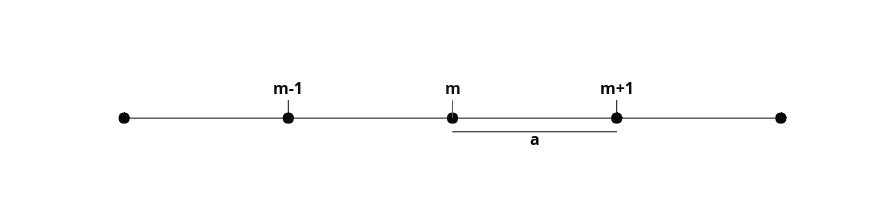
\includegraphics[scale=0.6]{imagenes/red.png}
    \caption{Red infinita homonuclear en una dimensión}
    \label{fig:5.1}
\end{figure}

La primera hipótesis para la construcción del modelo es que en cada sitio $n$, hay un solo orbital $\ket{n}$ que es ortogonal a todos los demás orbitales en los otros sitios de la red \cite{oxford}:

\begin{equation}\label{eq:5.1}
    \braket{n}{m}=\delta_{n,m}\,,
\end{equation}

Se supone adicionalmente que los estados constituyen conjunto completo, tal como se muestra a continuación:

\begin{equation}\label{eq:5.2}
    \sum_n \ket{n}\bra{n}=\mathbf{1}
\end{equation}

La última suposición acerca de la red, es que esta posee $N$ sitios y con condiciones de borde periódicas de Born–von Karman ($\ket{0}=\ket{N}$). Al estar los iones tan cerca unos de otros, la función de onda de cada orbital se superpone con las demás. Se puede escribir ésta función como la combinación lineal de todos los estados ortogonales\cite{oxford}:

\begin{equation}\label{eq:5.3}
    \ket{\Psi}=\sum_n \phi_n\ket{n}
\end{equation}

Donde los coeficientes se escriben de la siguiente manera:

\begin{equation}\label{eq:5.4}
    \phi_n=\braket{n}{\Psi}
\end{equation}

Se quiere, entonces, hallar una expresión para la energía de un electrón en la red, para esto se escribe la ecuación del Hamiltoniano para un electrón arbitrario en la posición $m$:

\begin{equation}\label{eq:5.5}
    H=\frac{\rho^2}{2m}+\sum_j V(\overline{r}-\overline{R_j})\,,
\end{equation}

Si $K=\frac{\rho^2}{2m}$ es la energía cinética del electrón y $V_j=V(\overline{r}-\overline{R_j})$ es el potencial que ejerce el ion en la posición $\overline{R_j}$ sobre el electrón en la posición $\overline{r}$, se puede reescribir el Hamiltoniano de este sistema de la forma siguiente:

\begin{equation}\label{eq:5.6}
    H=K+V_m+\sum_{j \neq m } V_j\,,
\end{equation}

Se observa que $K+V_m$ es el Hamiltoniano en ausencia de la red y solo el potencial del ion en la posición $m$ actúa sobre el electrón. Si se aplica $\ket{m}$ sobre \ref{eq:2.6} a ambos lados de la igualdad, se obtendrá:

\begin{equation}\label{eq:5.7}
    H\ket{m}=(K+V_m)\ket{m}+\sum_{j \neq m}V_j\ket{m}
\end{equation}

La ecuación de Schrödinger independiente del tiempo para un solo átomo es: 

\begin{equation}\label{eq:5.8}
    (K+V_m)\ket{m}=\epsilon_{atomico}\ket{m}
\end{equation}

Combinando \ref{eq:5.7} con \ref{eq:5.8} y aplicando $\bra{n}$ se obtienen las siguientes expresiones :

\begin{equation}\label{eq:5.9}
    \bra{n}H\ket{m}=\epsilon_{atomico}\delta_{n,m}+\sum_{j \neq m}\bra{n}V_j\ket{m}
\end{equation}

\begin{equation}\label{eq:5.10}
    H_{nm}=\epsilon_{atomico}\delta_{n,m}+\sum_{j \neq m}\bra{n}V_j\ket{m}
\end{equation}

Sean $\{\psi_1(x),\psi_2(x),\dots,\psi_n(x)\}$ el conjunto de funciones de onda ortogonales asociadas a los orbitales $\{\ket{1},\ket{2},\dots,\ket{n}\}$ que describen a cada electrón en la posición $n$. Cada función describe al electrón como un paquete localizado en la región alrededor de su posición $n$ y cuya probabilidad de estar en la posición mas lejana a $n \pm 1$ es nula (aproximación de primeros vecinos) \cite{ashc}:

\begin{equation}\label{eq:5.11}
    \sum_{j \neq m}\bra{n}V_j\ket{m}=\sum_{j \neq m}\int \psi_n^{*}(x)V_j(x)\psi_m(x)dx=\sum_{j \neq m}\int \psi_m^{*}(x)V_j(x)\psi_m(x-\abs{m-n}a)dx
\end{equation}


\begin{equation}\label{eq:5.12}
\sum_{j \neq m}\bra{n}V_j\ket{m}=
    \begin{cases}
    V_o & \text{si $m=n$}\\
    -A & \text{si $m=n\pm 1 $} \\
    0 & \text{en otro caso}
    \end{cases}
\end{equation}

\begin{equation}\label{eq:5.13}
    H_{nm}=\epsilon_{0}\delta_{n,m}-A(\delta_{n+1,m}+\delta_{n-1,m})
\end{equation}

Recordando el teorema de Bloch, para cada posición de la red, existirá una solución que cumple con el teorema; y, haciendo una combinación lineal de todas las soluciones obtiene la solución general de la red, como se expresa en la siguiente ecuación:

\begin{equation}\label{eq:5.14}
    \psi_{k,n}(x)=\sum_n e^{ikna}\psi_n(x-na)
\end{equation}

Esta es una función que toma en cuenta todos los niveles atómicos a lo largo del cristal. Sin embargo, una aproximación mas realista tomaría en cuenta solo algunos vecinos. Se define un $\phi$ tal que la función de onda de la red cristalina sea como se muestra a continuación: 

\begin{equation}\label{eq:5.15}
    \psi_{k,n}(x)=\frac{1}{N}\sum_n e^{ikna}\phi_n(x-na)
\end{equation}

Donde $\phi(x)$ solo puede representarse como una combinación lineal de $\psi_n$ para algunos pocos vecinos. Además $\phi(x)$ debe ser periódico, de periodo $a$ para que cumpla con la teoría de Floquet: 

\begin{equation}\label{eq:5.16}
    \phi(x)=\sum_n b_n\psi_n
\end{equation}

Siguiendo el procedimiento que se muestra en el apéndice \ref{apendice:B}, se puede obtener un valor para $\mathcal{E}(k)$:

\begin{equation}\label{eq:5.17}
    \mathcal{E}(k)=\mathcal{E}_0-2A\cos(ka)
\end{equation}

Donde A se denomina parámetro de "\textit{Hopping}", este parámetro indica la probabilidad del electrón de efectuar un salto a celdas vecinas. En el limite del continuo, cuando $a$ tiende a cero, este parámetro tiende a infinito, se entiende entonces que en el continuo no existen restricciones para el electrón de viajar en el espacio real o de aumentar o disminuir su energía puesto que no existirán bandas prohibidas. El valor $\mathcal{E}(k)$ que se acaba de hallar es la relación de dispersión del electrón en la red.
\chapter{Dinámica semiclásica del electrón en la red de Tight Binding en campos rápidamente oscilantes}

\section{Método de Kapitza en la dinámica clásica de una partícula en presencia de un campo externo rápidamente oscilante}\label{cap:6}

Se quiere estudiar el procedimiento de Kapitza para modelar partículas clásicas en presencia de fuerzas externas rápidamente oscilantes. El siguiente procedimiento sigue los presentados por Kapitza \cite{kapitza} y Landau \cite{landau},  para modelar la dinámica de partículas clásicas sometidas a campos rápidamente oscilantes.

La ecuación de movimiento de una partícula de masa $m$, que experimenta un potencial $U$ independiente del tiempo y una perturbación $f(x,t)$ rápida, está dada por la segunda ley de Newton: 

\begin{equation}\label{eq:6.1}
    m\ddot{x}=-\frac{\partial U(x)}{\partial x}+f(x,t)
\end{equation}

Se describe una fuerza externa que incluye todos los posibles armónicos de $\omega$ modulados por una función $f_n(x)$. Por simplicidad, se supone que $f_n(x)=f_{-n}(x)$ y se escribe como serie de Fourier, tal como se muestra a continuación:

\begin{equation}\label{eq:6.2}
    f(x, t) = \sum^{\infty}_{n=-\infty} f_n(x)e^{in\omega t},
\end{equation}

Donde $f_n(x)$ y $\omega$ son grandes comparados con las amplitudes y frecuencias naturales del movimiento lento. Por la naturaleza de las fuerzas, que actúan sobre la partícula, se puede deducir que la partícula efectúa un movimiento rápido debido a la fuerza oscilante; y al mismo tiempo, presenta un movimiento suave debido a la fuerza $U(x)$ de oscilación lenta.
Se puede separar el movimiento de la partícula en un movimiento rápido y otro lento. Esta situación se expresa matemáticamente con la expresión:

\begin{equation}\label{eq:6.3}
    x(t) = X(t) + \xi(t),
\end{equation}

Donde $\xi$ representa el movimiento rápido y se supone pequeño y de promedio cero en un periodo de movimiento rápido  ($T=2\pi/\omega$). Se supone, también, que en períodos de tiempo pequeños  los cambios de $X(t)$ son insignificantes. 

Sustituyendo la ecuación \ref{eq:6.3} en \ref{eq:6.1}, y expandiendo el lado derecho de la ecuación \ref{eq:6.1} en serie de Taylor alrededor de $\xi=0$ a primer orden, se tiene la ecuación:

\begin{equation}\label{eq:6.4}
    m(\ddot{X}(t) + \ddot{\xi}(t))=-\frac{\partial U(X)}{\partial X}-\xi\frac{\partial^2 U(X)}{\partial X^2}+f(X,t)+\xi\frac{\partial f(X,t)}{\partial X}
\end{equation}

Las derivadas en el tiempo que aparecen en \ref{eq:6.4} son funciones suaves, en el sentido que no varían mucho para tiempos del orden del periodo pequeño. Se puede separar entonces los movimientos rápido y lento de la siguiente manera:

\begin{equation}\label{eq:6.5}
    m\ddot{X}(t) =-\frac{\partial U(X)}{\partial X}-\xi\frac{\partial^2 U(X)}{\partial X^2}+\xi\frac{\partial f(X,t)}{\partial X}
\end{equation}

\begin{equation}\label{eq:6.6}
    m\ddot{\xi}(t)=f(X,t)
\end{equation}

Se integra, la ecuación \ref{eq:6.6} en la variable temporal y se obtiene una expresión  para $\xi$ (suponiendo condiciones iniciales apropiadas que anulan el término secular):

\begin{equation}\label{eq:6.7}
    \xi=-\frac{1}{m\omega^2}\sum^{\infty}_{n=-\infty} \frac{f_n(X)e^{in\omega t}}{n^2}
\end{equation}
 
Conociendo una expresión para $\xi$, se puede ahora calcular el valor promedio de $\ddot{x}(t)$ en un periodo rápido, teniendo en cuenta que $\overline{\ddot{\xi}(t)}=0$:

\begin{equation}\label{eq:6.8}
    m\overline{\ddot{X}}(t) =-\overline{\frac{\partial U(X)}{\partial X}}-\overline{\xi\frac{\partial^2 U(X)}{\partial X^2}}+\overline{\xi\frac{\partial f(X,t)}{\partial X}}
\end{equation}

Recordando que $U(X)$ se considera constante para periodos pequeños y que $\xi$ tiene promedio nulo en ese mismo periodo. Además, se puede calcular $\overline{\xi\frac{\partial f(X,t)}{\partial X}}$ y obtener la siguiente ecuación:

\begin{equation}\label{eq:6.9}
     m\overline{\ddot{X}}(t) =-\frac{\partial U}{\partial X}-\frac{1}{2m\omega^2}\frac{\partial}{\partial X}\sum_n \frac{f_n^2(X)}{n^2}
\end{equation}

Se puede definir el potencial efectivo de una partícula sometida a fuerzas rápidamente oscilantes como se presenta en el resultado \ref{eq:6.11}:

\begin{equation}\label{eq:6.10}
    m\overline{\ddot{X}}=-\frac{\partial U_{eff}(X)}{\partial X}
\end{equation}

\begin{equation}\label{eq:6.11}
U_{eff}(X)=U(X)+\frac{1}{2m\omega^2}\sum_n \frac{f_n^2(x)}{n^2}   
\end{equation}

Se observa que el potencial experimenta una corrección que es inversamente proporcional a la masa y al cuadrado de la frecuencia de la fuerza rápidamente oscilante. Además es directamente proporcional a la suma del modulo cuadrado de los armónicos de la fuerza y que la corrección tiene una dependencia en $X$. En el límites $\omega \rightarrow \infty$ el término de corrección del potencial se hace insignificante y el efecto de la fuerza externa sobre la dinámica de la partícula será nulo.

%%%%%%%%%%%%%%%%%%%%%%%%%%%%%%%%%%%%%%%%%%%%%%%%%%%%
\section{Dinámica semiclásica del electrón en la red de enlace fuerte en presencia de campos externos}\label{cap:7}

%En este capitulo se estudia el modelo semiclásico para la dinámica del electrón en la red. Este modelo permite predecir de forma sencilla el comportamiento del electrón en la red en presencia de campos externos, sin embargo existen ciertas condiciones que limitan la aplicación de este modelo, las cuales son aclaradas. Se presenta el concepto de masa efectiva del electrón y la deducción de su expresión matemática a partir de las ecuaciones de movimiento semiclásicas. Se presenta además la aplicación del modelo semiclásico para el caso del electrón en la red en presencia de un potencial perturbativo lineal, cuyo resultado son las oscilaciones de Bloch. Este capítulo abre el camino para el estudio semiclásico que se presenta mas adelante sobre el electrón en la red en presencia de campos rápidamente oscilantes (capítulo \ref{cap:9}). 

El modelo semiclásico describe la respuesta de los electrones en la red a un campo externo aplicado. Para que este modelo sea válido, las variaciones del campo en el espacio deben ser muy pequeñas comparadas con las dimensiones del paquete de onda del electrón. Estos campos dan origen a fuerzas clásicas que describen el movimiento del paquete de onda. La segunda condición en el modelo semiclásico es que la periodicidad de la red debe ser pequeña comparada con las dimensiones del paquete de onda del electrón. En esta situación, el potencial de la red no puede tratarse clásicamente (ver figura \ref{fig:7.1}). Por lo tanto, el modelo semiclásico trata las fuerzas externas clásicamente, mientras que el potencial cristalino es tratado cuánticamente \cite{ashc}.

\begin{figure}[H]
    \centering
    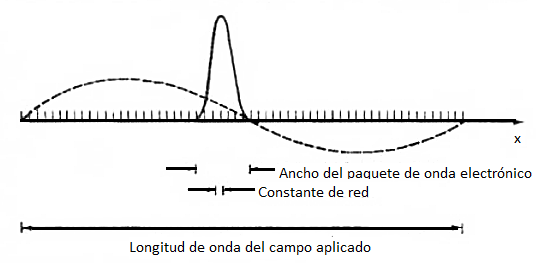
\includegraphics[scale=.9]{imagenes/dinamica-semiclasica.png}
    \caption{Electrón en una red periódica en presencia de un potencial periódico externo, Modificado de Ashcroft y Mermin \cite{ashc} }
    \label{fig:7.1}
\end{figure}

El modelo semiclásico, describe (en ausencia de colisiones) la velocidad $\dot{x}$ y la fuerza $\hbar k$, que experimenta el paquete de onda del electrón en presencia de un campo externo; esta predicción es posible en conocimiento de la relación de dispersión $\mathcal{E}_n(k)$. Dada la función $\mathcal{E}_n(k)$ el modelo semiclásico permite calcular la posición $x$ y el vector de onda $k$ asociado a éste para una banda $n$. En presencia de campos eléctricos $E(x,t)$ y magnéticos $\mathcal{H}(x,t)$ la posición y el vector de onda pueden ser calculados siempre y cuando la posibilidad de intercambio de banda $n$ sea descartada. Entonces las ecuaciones de movimiento del electrón serán las siguientes:

\begin{equation}\label{eq:7.1}
    \dot{\textbf{x}}=\textbf{v}_n(k)=\frac{1}{\hbar}\frac{\partial \mathcal{E}_n(k)}{\partial k}
\end{equation}

\begin{equation}\label{eq:7.2}
    \hbar\dot{\textbf{k}}=-e\left[\textbf{E}(x,t)+\frac{1}{c}\textbf{v}_n(k)\times \mathcal{H}(x,t)\right]
\end{equation}

En el modelo semiclásico, no puede haber dos electrones cuyos valores de $k$ difieran por una constante de red reciproca $K$, puesto que las funciones que describen al electrón son periódicas, de periodo $K$, y en consecuencia se estaría hablando del mismo electrón \cite{ashc}.

El método de Kapitza, usando el enfoque semiclásico permite crear un nuevo modelo que describe la dinámica del electrón en la red en presencia de campos rápidamente oscilantes. Mas adelante se encontrará que es posible obtener una fórmula general del potencial efectivo para el electrón en presencia de cualquier potencial que cumpla con las condiciones semiclásicas que se han estudiado en esta sección (capítulo \ref{cap:9}).

\subsection{Masa efectiva}

Se puede describir la manera como un electrón responde a fuerzas externas definiendo una nueva cantidad llamada masa efectiva del electrón:

\begin{equation}\label{eq:7.3}
    \frac{1}{m^*}=\frac{1}{\hbar^2}\frac{\partial^2 \mathcal{E}(k)}{\partial k^2}
\end{equation}

Esta ecuación se obtiene de las ecuaciones del movimiento semicásico del electrón
e implica que es posible para el electrón tener masa efectiva positiva o negativa. La masa efectiva es positiva cuando la relación de dispersión tenga una curvatura hacia arriba y negativa cuando la curvatura sea hacia abajo, incluso puede haber masa cero en los puntos de inflexión de la curva.

Para un electrón libre la relación de dispersión tiene la expresión cuadrática:

\begin{equation}\label{eq:7.4}
    \mathcal{E}(k)=\frac{\hbar^2k^2}{2m}
\end{equation}

Entonces la masa efectiva, como es de esperarse, es la misma que la masa regular del electrón:

\begin{equation}\label{eq:7.5}
    m^*=m
\end{equation}

Para un electrón en la red de \textit{Tight Binding} la relación de dispersión tiene una forma totalmente diferente a la del electrón libre:

\begin{equation}\label{eq:7.6}
    \mathcal{E}(k)=\mathcal{E}_0-2A\cos(ka)
\end{equation}

En consecuencia la masa efectiva del electrón en la red de \textit{Enlace Fuerte}, tomando $\hbar$=1, resulta ser:

\begin{equation}\label{eq:7.7}
    m^*=(2Aa^2\cos(ka))^{-1}
\end{equation}

A continuación se presenta un gráfico referencial de la masa efectiva del electrón en la red de enlace fuerte como función de $k$, se ha dibujado también la curva de la relación de dispersión para que se pueda apreciar la relación entre ambas.

\begin{figure}[H]
    \centering
    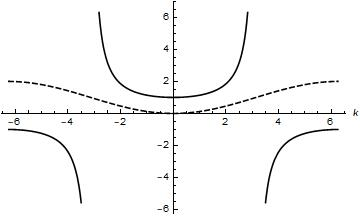
\includegraphics{imagenes/masa-efectiva.jpg}
    \caption{Linea solida: Masa efectiva, Linea discontinua: Relación de dispersión}
    \label{fig:my_label}
\end{figure}

En la figura se puede observar que el cambio de concavidad en la curva de relación de dispersión provoca un cambio de signo en la masa efectiva del electrón en la red de \textit{Tight Binding}. Este cambio de signo también se puede interpretar como un cambio de signo en la carga del electrón, pasando de ser atraído por el pozo de potencial a ser repelido por este en la zona de masa efectiva negativa.

\subsection{Oscilaciones de Bloch}\label{cap:7.2}

En 1928, Bloch demostró teóricamente que un paquete de ondas electrónicas, compuesto por una superposición de estados de una sola banda, bajo la acción un campo eléctrico externo aplicado alcanza su punto máximo en un determinado cuasi momentum $k$ y presenta oscilaciones periódicas en el momento y el espacio real, si se descartan las transiciones entre bandas \cite{Shah}.

La dinámica de los electrones de Bloch en un campo eléctrico homogéneo es un problema de larga data en el estudio en la \textit{Física del Estado Sólido}, si se considera un electrón sin colisión en una red periódica en una dimensión, con un movimiento normal a los planos de la superred. La ecuación de movimiento del electrón en presencia de un campo eléctrico uniforme $E$, paralelo a k, se escribe según las ecuaciones siguientes: 

\begin{equation}\label{eq:7.8}
    \frac{\hbar dk}{dt} = -eE
\end{equation}

\begin{equation}\label{eq:7.9}
    k(t)=k_0-\frac{eEt}{\hbar} 
\end{equation}

El electrón, se mueve hasta alcanzar el punto máximo de la banda, entonces es reflejado por ésta en la frontera de la \textit{Zona de Brillouin} (\textit{Reflexión de Bragg}) e invierte su movimiento. En el caso ideal, se puede ignorar por completo la dispersión causada por los iones de la red o imperfecciones y el electrón efectúa \textit{Oscilaciones de Bloch} de periodo dado por la ecuación \ref{eq:7.9}, donde $a$ es la constante de la red y $h$ la constante de Planck.

\begin{equation}\label{eq:7.10}
    \tau_B=\frac{\hbar}{eEa}
\end{equation}

Se considera el movimiento del electrón en el espacio real con la relación de dispersión en el \textit{Enlace Fuerte} y la expresión para la velocidad del electrón en el modelo semiclásico \cite{kittel}:

\begin{equation}\label{eq:7.11}
\mathcal{E}(k)=\mathcal{E}_o-2A\cos(ka)   
\end{equation}

\begin{equation}\label{eq:7.12}
v=\frac{1}{\hbar}\frac{d\mathcal{E}}{dk}
\end{equation}

Sustituyendo el resultado \ref{eq:7.11} en \ref{eq:7.12} se puede obtener la posición del electrón en función del tiempo, que resulta ser una función periódica con período de oscilación $\tau_B$:

\begin{equation}\label{eq:7.13}
    x=-\frac{2A}{Ee}\cos(\frac{aeE}{\hbar}t)
\end{equation}

 Este resultado confirma la existencia teórica de las oscilaciones de Bloch cuya frecuencia en el espacio real es $\omega_B=\hbar/aeE$, y período igual a $\tau_B$. Se encuentra entonces que la respuesta del electrón en la red a un potencial lineal externo es totalmente diferente que en el espacio libre, para el cual la aceleración producida por un campo eléctrico homogéneo es constante \cite{kittel}. En este caso, el electrón experimenta oscilaciones alrededor de un punto de equilibrio.
 
En la ecuación \ref{eq:7.3} se observa que cuanto mayor sea la magnitud del campo eléctrico externo, la amplitud de las oscilaciones y el periodo de Bloch son menores. Por lo tanto la probabilidad de que el electrón sufra algún tipo de dispersión antes de terminar una oscilación de Bloch es menor. Las oscilaciones de Bloch son difíciles de observar experimentalmente en un sólido cristalino, debido a que la dispersión por impurezas o fonones impide la finalización de un solo período de oscilación \cite{raizen}. Esto hizo que la investigación en el campo de la dinámica oscilatoria de electrones en los sólidos haya tenido durante muchos años un interés sobre todo teórico. La obtención en los últimos años de materiales con constante de red $a$ de ordenes diez veces mayor a las convencionales y menor presencia de impurezas ha aumentado el atractivo de esta área de la Física del Estado Sólido \cite{wannier2}. Una de las condiciones para la observación de las oscilaciones de Bloch, es que el período de oscilación $\tau_B$ debe ser menor que el tiempo medio de viaje $\tau_m$, de lo contrario, el electrón experimentará una dispersión antes de poder observar alguna oscilación.


Para este proyecto de grado se ha querido considerar campos externos inhomogéneos y rápidamente oscilantes, con la finalidad de estudiar la dinámica del electrón en presencia de estos campos y observar posibles fenómenos oscilatorios y de localización del paquete de onda del electrón.

\chapter{Dinámica cuántica del electrón en la red bajo el efecto de campos externos oscilantes}

\section{Método de Floquet-Magnus}\label{cap:8}

En este capítulo, se estudia un método que permite modelar la dinámica cuántica del electrón bajo la influencia de Hamiltonianos dependientes del tiempo. Se quiere obtener un Hamiltoniano efectivo independiente del tiempo, usando la expansión de Floquet-Magnus.  

Wilhelm Magnus (1907-1990) fue un matemático americano-alemán, con importantes contribuciones a la \textit{Teoría Combinatoria de Grupos}, \textit{Álgebra de Lie}, \textit{Física Matemática} y \textit{Funciones Elípticas}. Su libro, ''\textit{Hill's Equations}'' ha sido clave en la realización de este trabajo. La expansión de Floquet-Magnus es una aproximación útil para resolver ecuaciones diferenciales lineales dependientes del tiempo; las cuales son un problema común en Física Cuántica y Física del Estado Sólido. Estas ecuaciones son tratadas con teoría de Hamiltonianos efectivos y de Floquet \cite{mananga}.
La expansión de Floquet-Magnus es una nueva versión de la expansión de Magnus \cite{maricq}; Maricq, en su trabajo, desarrolla una formula recursiva para obtener los términos de la expansión y da las condiciones para su convergencia \cite{mananga}.

Se puede extender la Teoría de Floquet a Hamiltonianos periódicos en el tiempo. Siguiendo los cálculos hechos por Maricq en 1982 \cite{maricq}, y posteriormente por Martínez en 2017 \cite{martinez2017} se hallan soluciones independientes del tiempo para la dinámica de un electrón en la red que experimenta una perturbación dependiente del tiempo.

\subsection{Expansión de Floquet-Magnus}\label{cap:8.1}

Se define la ecuación de Schrödinger dependiente del tiempo, con Hamiltoniano periódico $H(t)$:

\begin{equation}\label{eq:8.1}
    \frac{dU(t)}{dt}=-iH(t)U(t)
\end{equation}

La misma tiene la solución dada por la Teoría de Floquet y cumple con el teorema \ref{teo:2.1} (sección \ref{cap:2}). En consecuencia, se sabe que existe un $P(t)$ periódico, con periodo $\tau$ tal que se cumple:

\begin{equation}\label{eq:8.2}
    U(t+\tau)=U(t)e^{-i\overline{H}\tau}
\end{equation}

\begin{equation}\label{eq:8.3}
    U(t)=P(t)e^{-i\overline{H}t}
\end{equation}

El Hamiltoniano efectivo (independiente del tiempo) del sistema es el operador $\overline{H}$ y, $P(t)$ y $\overline{H}$ se definen bajo el esquema de perturbación \cite{maricq} como expansiones en serie de orden $\lambda$:

\begin{equation}\label{eq:8.4}
    P(t)=\sum_n \lambda^{n}P_n(t)
\end{equation}

\begin{equation}\label{eq:8.5}
    \overline{H}=\sum_n \lambda^n\overline{H_n}
\end{equation}

Se definen, además, los términos de orden cero  como en \ref{eq:8.6} \cite{maricq}\cite{martinez2017}. Y, siguiendo el procedimiento del apéndice \ref{apendice:C} se obtienen las expresiones para $P(t)$ y $\overline{H(t)}$; mismas que obtuvo Maricq en su trabajo \cite{maricq}, teniendo así, una expresión para Hamiltonianos efectivos de sistemas sometidos a Hamiltonianos dependientes del tiempo: 

\begin{equation}\label{eq:8.6}
    P_0(t)=1, \ \overline{H_0}=0
\end{equation}

\begin{equation}\label{eq:8.7}
    P_n(t)=-i\int^{t}_{0}\left[ H(t')P_{n-1}(t')-\sum^{n-1}_{k=1}P_k(t')\overline{H_{n-k}}-\overline{H_n}\right]
\end{equation}

\begin{equation}\label{eq:8.8}
    \overline{H_n}=\frac{-i}{\tau}\int^{\tau}_{0}\left[ H(t)P_{n-1}(t')-\sum^{n-1}_{k=1}P_k(t')\overline{H_{n-k}}\right]
\end{equation}

\subsection{Convergencia de la expansión}\label{cap:8.2}

Las expresiones de $P(t)$ y $\overline{H}$ constituyen una serie de soluciones formales para la ecuación \ref{eq:3.1} con la condición que $P(t)$ es periódica, con periodo $\tau$. Sin embargo, es necesario probar la convergencia de estas series para poder afirmar que son soluciones analíticas \cite{maricq}. Se consideran ecuaciones diferenciales de la siguiente forma:

\begin{equation}\label{eq:8.9}
    F(x, y, y') = 0
\end{equation}

Donde $x$ es de variable compleja $y(x)$ o una función vectorial compleja. Además $F$ es también una función vectorial de variable compleja, definida analítica en el vecindario de $(x_0,y_0,y'_0)$ y $F(x_0,y_0,y'_0)=0$. El problema de hallar soluciones analíticas cerca de $(x_0,y_0,y'_0)$ se divide en una parte algebraica y otra analítica. La parte algebraica consiste en la construcción, o al menos, la prueba de la existencia de una solución formal de la forma:

\begin{equation}\label{eq:8.10}
    u=\sum^{\infty}_{n=0}a_n(x-x_0)^n  ,   \ a_0=y_0 \ y \ a_1=y'_0
\end{equation}

La solución $u$ es llamada formal porque es una serie de potencias formal (no necesariamente convergente dentro de un radio positivo de convergencia), que satisface \ref{eq:8.9} en el sentido que su substitución del lado izquierdo de la formula da como resultado cero del lado derecho de la misma. La parte analítica del problema consiste en probar que la solución formal $u$ es la  solución verdadera de \ref{eq:8.9}, e idealmente converge. Las soluciones formales solo serán significativas para \ref{eq:8.9} si son asintóticas \cite{hautus}.

Determinar la convergencia de las series \ref{eq:8.4} y \ref{eq:8.5} presenta una dificultad, ya que ambas son interdependientes \cite{maricq}. Se aplica entonces una forma indirecta de probar su convergencia. De la ecuación \ref{eq:8.3} y de la periodicidad de $P(t)$ se obtiene que:

\begin{equation}\label{eq:8.11}
    U(\tau)=e^{-i\overline{H}\tau}
\end{equation}

Se puede reescribir  $U(t)$ por el método de aproximaciones de Picard \cite{ravi}\cite{maricq}, de la siguiente manera:

\begin{equation}\label{eq:8.12}
    U_0(t)=1
\end{equation}

\begin{equation}\label{eq:8.13}
    U_{n+1}(t)=1-i\int^{t}_0 \lambda H(t)U_n(t)dt
\end{equation}

Esta secuencia iterativa produce (por inducción) una serie de potencias en $\lambda$ de la siguiente forma:

\begin{equation}\label{eq:8.14}
    U_k(t)=1-i\lambda\int^{t}_0H(t)dt+\dots +i^k\lambda^k\int^{t}_0H(t_k)\dots \int^{t}_0H(t_1)dt_1 \dots dt_k
\end{equation}

Como $H(t)$ es una función acotada periódica, se dice por simplicidad y sin pérdida de generalidad, que el Hamiltoniano $H(t)$ está acotado por $1$. Usando esta condición e integrando varias veces, se obtiene que  $U_k-U_{k-1}$ (apéndice \ref{apendice:C}) cumple que: 

\begin{equation}\label{eq:8.15}
    \norm{U_k-U_{k-1}}\leq \frac{\lambda^kt^k}{k!}
\end{equation}

Se encuentra entonces que a medida que $k$ crece el error disminuye drásticamente, y $U_k$ converge. Por ende, $e^{-i\overline{H}\tau}$ debe converger, entonces $\overline{H}$ converge. En consecuencia la solución de Floquet  $U(t)=P(t)e^{-i\overline{H}t}$ converge. 

Se halla que existe una solución analítica $U(t)$ de \ref{eq:8.1} definida como en \ref{eq:8.3} y que además la serie de Floquet-Magnus converge. Por ende, es posible usar la base matemática desarrollada en este capítulo para encontrar soluciones aproximadas a las ecuaciones de Schrödinger periódicas dependientes del tiempo. 
\chapter{Método de Kapitza en la dinámica semiclásica del electrón en la red de enlace fuerte sometido a potenciales rápidamente oscilantes}\label{cap:9} 

En este capítulo se estudia la dinámica semiclásica de un electrón en la red en presencia de un campo externo rápidamente oscilante, los resultados que se obtienen en este capítulo forman parte de los resultados de este proyecto de grado. Para el desarrollo de estos cálculos se hace uso del método semiclásico para modelar la dinámica de un electrón en una red de \textit{Tight Binding} en presencia de un campo externo, combinado con el método de Kapitza para la dinámica clásica de una partícula en presencia de fuerzas rápidamente oscilantes. Se sigue el procedimiento de Maricq para resolver la dinámica del electrón en una red de \textit{Tight Binding} y en presencia de un potencial externo rápidamente oscilante \cite{maricq}\cite{mart2014}.

%%%%%%%%%%%%%%%%%%%%%%%%%%%%%%%%%%%%%%%%%%

Se presenta el problema de un electrón en una red unidimensional, bajo la influencia de un campo eléctrico externo inhomogéneo y rápidamente oscilante. Esto es, la frecuencia de oscilación de este campo externo es mucho mayor que $\omega_{0}$. Las perturbaciones dependientes del tiempo, como la que se presenta, han sido estudiadas extensamente \cite{Dunlap}\cite{mart2014}. Si el movimiento está gobernado por las leyes de la mecánica clásica y la perturbación es rápida, intensa y periódica, existe un método desarrollado por Kapitza \cite{kapitza} y que se puede encontrar en el libro de Mecánica de Landau \cite{landau} que muestra es posible separar el movimiento en dos escalas de tiempo: una lenta gobernada por el sistema y una rápida como consecuencia de la perturbación. El uso de este modelo permite encontrar una dinámica efectiva independiente del tiempo para la partícula.

La dinámica de un electrón en la red, en presencia de un campo externo, puede ser estudiada a través de modelos semiclásicos \cite{ashc}, tal como se ha tratado en la sección \ref{cap:7} combinado con el metodo de Kapitza tratado en la sección \ref{cap:6}. En esta sección, se incluirán los resultados del modelo de \textit{Tight Binding} para hallar un modelo semiclásico que describa la dinámica de electrón.

Sea $U(x)$ un potencial que no depende del tiempo y $V(x,t)$ un potencial inhomogéneo que varía rápidamente en el tiempo ($\omega \gg \omega_o$). Las ecuaciones de movimiento del electrón en el modelo semiclásico están dadas por las siguientes ecuaciones:

\begin{equation}\label{eq:9.1}
    \dot{k}=\frac{-dU(x)}{dx}+f(x,t)
\end{equation}

\begin{equation}\label{eq:9.2}
    \dot{x}=2Aa\sin(ak)
\end{equation}
    
Donde la fuerza se ha definido como $f(x,t)=-\partial_x V(x,t)$. Se escribe la fuerza externa como una serie de Fourier (ecuación \ref{eq:9.3}) y se imponen las siguientes condiciones sobre ella:

\begin{enumerate}
    \item El promedio de $f(x,t)$ en un periodo de oscilación rápida es $\overline{f(x,t)}=0$
   \item $f_n(x)=f_{-n}(x)$ (Paridad)
\end{enumerate}

\begin{equation} \label{eq:9.3}
    f(x,t)=\sum_{-\infty}^{\infty} f_n(x) e^{i n\omega t}
\end{equation}
    
Se puede representar el movimiento total de la partícula como la suma de dos movimientos independientes: uno rápido ($\xi(t)$), de amplitud pequeña, y otro lento ($X(t)$) de mayor amplitud \cite{landau}. Esta situación se describe de la siguiente manera:
   
\begin{equation}\label{eq:9.4}
    x=X(t)+\xi(t)
\end{equation}
   
\begin{equation}\label{eq:9.5}           
    k=K(t)+\eta(t)
\end{equation}
    
Donde $\overline{\eta}=\overline{\xi}=0$. Se derivan las ecuaciones \ref{eq:9.4} y \ref{eq:9.5} para obtener las velocidades del sistema. Y, al derivar de nuevo para obtener la aceleración, se acoplan ambas ecuaciones para obtener la aceleración del electrón:
    
\begin{equation}\label{eq:9.6}
    \dot{X}+\dot{\xi}=2Aa\sin(ak)
\end{equation}
    
\begin{equation}\label{eq:9.7}               \dot{K}+\dot{\eta}=-\frac{dU}{dx}+f(x,t)
\end{equation}

\begin{equation}\label{eq:9.8}
    \ddot{X}+\ddot{\xi}=2Aa\cos(ak)\times\dot{k}
\end{equation}

\section{Separación de movimientos rápido y lento}\label{cap:9.1.1}

Se obtuvo una expresión para la aceleración, la cual no puede ser separada (de momento) en movimientos rápido y lento. Se sigue un procedimiento que permite separar estos movimientos de acuerdo al método usado por Kapitza \cite{kapitza}. En primer lugar, se sustituye las ecuaciones \ref{eq:9.1} y \ref{eq:9.5} en \ref{eq:9.8}:
 
\begin{equation}\label{eq:9.9}
    \ddot{X}+\ddot{\xi}=2Aa^2\cos((K+\eta)a)\times(-\frac{dU}{dx}+f(x,t))
\end{equation}
    
Usando la siguiente identidad trigonométrica y sustituyendo en la ecuación \ref{eq:9.9} se obtiene:

$$\cos(a+b)=\cos(a)\cos(b)-\sin(a)\sin(b)$$

\begin{equation}\label{eq:9.10}
    \ddot{X}+\ddot{\xi}=2Aa^2(\cos(Ka)\cos(\eta a)-\sin(Ka)\sin(\eta     a))\times(-\frac{dU}{dx}+f(x,t))
\end{equation}

 Siguiendo el procedimiento de Landau \cite{landau} se expande en serie de Taylor $\frac{dU}{dx}$ y $f(x,t)$ alrededor de $\xi=0$ a primer orden, para conocer como actúan estas fuerzas en la zona del movimiento oscilatorio rápido.

\begin{equation}\label{eq:9.11}
    \frac{dU}{dx}=\frac{dU}{dX}+\xi\frac{d^2U}{dX^2}
\end{equation}
    
\begin{equation}\label{eq:9.12}
    f(X,t)=f(X,t) + \xi \frac{\partial f(X,t)}{\partial X} 
\end{equation}

Sustituyendo la expresión \ref{eq:9.11} y \ref{eq:9.13} en \ref{eq:9.10} se obtiene lo siguiente: 
    
\begin{equation}\label{eq:9.13}
    \begin{split} 
        &\ddot{X}+\ddot{\xi}=2Aa^2\left(\cos(Ka)\cos(\eta a)-\sin(Ka)\sin(\eta a)\right)(-\frac{dU}{dX}-\xi\frac{d^2U}{dX^2}+ \\ &+f(X,t) + \xi \frac{\partial f(X,t)}{\partial X} )
    \end{split}
\end{equation}

Tomando $\xi$ muy pequeño, se pueden separar los movimientos rápido y lento como en las siguientes expresiones:

\begin{equation}\label{eq:9.14}
    \ddot{\xi}=2Aa^2\left(\cos(Ka)\cos(\eta a)-\sin(Ka)\sin(\eta a)\right)f(X,t)
\end{equation}

\begin{equation}\label{eq:9.15}
   \ddot{X}=2Aa^2\left(\cos(Ka)\cos(\eta a)-\sin(Ka)\sin(\eta a)\right)\left(-\frac{dU}{dX}-\xi\frac{d^2U}{dX^2} + \xi \frac{\partial f(X,t)}{\partial X} \right)
\end{equation}

Este producto se resuelve, para luego calcular el promedio para un periodo en la oscilación pequeña, donde se tiene que $\overline{\ddot{X}}=\ddot{X}$. Haciendo uso de los promedios calculados en el apéndice \ref{apendice:B.4}, se obtiene que la aceleración efectiva del electrón en la red, en presencia de un campo externo rápidamente oscilante, esta dado por:

\begin{equation}\label{eq:9.16}
 \ddot{X}= -2Aa^2\cos(Ka)\left[\left(1-\frac{a^2}{2}\sum_n \frac{f_n^2(X)}{\omega^2n^2}\right)\frac{dU}{dX}+2Aa^2\cos(Ka)\sum_n \frac{1}{2n^2\omega^2}\frac{\partial f_n^2(X)}{\partial X}\right]
\end{equation}

Donde $m^*=(2Aa^2\cos(Ka))^{-1}$ es la masa efectiva del electrón en la red de enlace fuerte, por lo tanto, la formula general para la aceleración efectiva es:

\begin{equation}\label{eq:9.17}
 \ddot{X}= -\frac{1}{m^*}\left(1-\frac{a^2}{2}\sum_n \frac{f_n^2(X)}{\omega^2n^2}\right)\frac{dU}{dX}-\frac{1}{2m^{*2}\omega^2}\sum_n \frac{1}{n^2}\frac{\partial f_n^2(X)}{\partial X}
\end{equation}

\section{Calculo del potencial efectivo}\label{cap:9.1.2}

De la ecuación \ref{eq:9.17} es posible obtener el potencial efectivo:

\begin{equation}\label{eq:9.18}
    U_{eff}= U(X)-\frac{a^2}{2\omega^2}\sum_n \frac{f_n^2(X)}{n^2}U(X)+\frac{1}{2m^{*}\omega^2}\sum_n \frac{f_n^2(X)}{n^2} 
\end{equation}

Estos resultados se asemejan a los obtenidos por Malay Bandyopadhyay et al. \cite{datta} salvo el segundo término, el cual se explica por la presencia de la relación de dispersión de \textit{Tight Binding} en las ecuaciones de movimiento del electrón. Obsérvese que debido al efecto de la fuerza oscilante, tendremos una corrección en el potencial experimentado por la partícula, cuyo valor, se ha aproximado hasta términos de $\omega^{-2}$.

Se observa que en el límite del continuo $m^* \rightarrow m$ y el potencial efectivo toma la forma exacta del resultado de Malay Bandyopadhyay et al.: 

\begin{equation}\label{eq:9.19}
    \lim_{a\rightarrow 0}U_{eff}= U(X)+\frac{1}{2m\omega^2}\sum_n \frac{f_n^2(X)}{n^2} 
\end{equation}

Este resultado difiere del obtenido por Martínez et al.(2014) \cite{mart2014}, se usó una aproximación diferente al del citado artículo para calcular el potencial efectivo, ya que se encontró que las variables $\eta$ y $\xi$ no son independientes entre sí, en consecuencia no se puede calcular los promedios por separado de los factores de la ecuación \ref{eq:9.15} para luego expandir el producto. 

\section{Obtención de una cantidad conservada en la dinámica del electrón en la red en presencia de un campo externo rápidamente oscilante}\label{cap:9.2}

Se ha hallado una expresión para la aceleración efectiva del electrón y el potencial efectivo del electrón. Se puede hallar además, tal como encontró Martínez et al. (2014) una cantidad conservada para el movimiento del electrón en este sistema.

Se comenzará calculando $\dot{X}/\dot{K}$ siguiendo procedimiento de Martínez (2014) \cite{mart2014}: 
\begin{equation}\label{eq:9.20}
    \frac{dX}{dK}=\frac{-2A\sin(Ka)\overline{\cos(\eta a)}}{-\frac{\partial U}{\partial X}+\xi \overline{\frac{\partial f(X)}{\partial X}}}
\end{equation}

Del apéndice \ref{apendice:B} se obtiene el siguiente resultado:

    \begin{equation}\label{eq:9.21}
        \overline{\xi \frac{\partial f(X,t)}{\partial X}}=2A\cos(Ka)\frac{\partial\overline{cos(\eta a)}}{\partial X}
    \end{equation}
 
 De la ecuación \ref{eq:9.20} se obtiene la forma del diferencial total $d\left(-2A\cos(Ka)\overline{\cos(\eta a)}+U(X)\right)$, tomando en cuenta el resultado \ref{eq:9.21} se encuentra que el diferencial total es idéntico a cero:
 
 \begin{equation}
    \begin{split}
     0&=\frac{\partial}{\partial X} \left(-2A\cos(Ka)\overline{cos(\eta a)}+U(X)\right)dX+\frac{\partial}{\partial K}\left(-2A\cos(Ka)\overline{cos(\eta a)}\right)\\
     &=d\left(2A\cos(Ka)\overline{cos(\eta a)}+U(X)\right)
     \end{split}
 \end{equation}
 
 Se encuentra una cantidad conservada para el electrón en el sistema que se denotará por $\mathcal{E}$
 
    
\begin{equation}\label{eq:9.24}
    \mathcal{E}=-2A\cos(aK)+U(X)+2Aa^2\cos(Ka)\sum_n\frac{f_n^2(X)}{2n^2\omega^2}
\end{equation}  

Cuyo resultado, coincide con el resultado del trabajo de Malay Bandyopadhyay et al. \cite{datta} para el Hamiltoniano efectivo, usando el método de \textit{Rahav et al.}. Se puede inferir que la cantidad que se conserva es en realidad el Hamiltoniano efectivo del electrón. El resultado \ref{eq:9.24} puede resumirse como: 

\begin{equation}\label{eq:9.25}
    H(X,K)=H_0(X,K)+\frac{1}{2\omega^2m^*}\sum_n\frac{f_n^2(X)}{n^2}
\end{equation}

Donde $H_0(X,K)$ es el Hamiltoniano en la red de \textit{Tight Binding} en ausencia del campo externo rápidamente oscilante.

\begin{equation}\label{eq:9.26}
    H_0(X,K)=-2A\cos(aK)+U(X)
\end{equation}


\section{Masa efectiva}

Es posible calcular la masa efectiva del electrón en este sistema ($m^{**}$) haciendo uso de la definición de masa efectiva.

\begin{equation}
    m^{**}=\frac{1}{2Aa^2\cos(Ka)}\left(1+\frac{a^2}{2}\sum_n \frac{f_n^2(X)}{\omega^2n^2}\right)
\end{equation}

Se obtiene además que en el limite del continuo la masa efectiva resulta ser la masa del electrón libre, como es de esperar.

\begin{equation}
    \lim_{a \rightarrow 0}m^{**}=m
\end{equation}

%%%%%%%%%%%%%%%%%%%%%%%%%%%%%%%%
\section{Aplicación del resultado semiclásico al caso lineal}

Se hace uso de los resultados generales obtenidos para modelar la dinámica del electrón en la red en presencia de un potencial eléctrico lineal que varia periódicamente con frecuencia $\omega$. El Hamiltoniano del electrón en este sistema es;

\begin{equation}\label{eq:9.28}
  H=-2A\cos(k a)+\epsilon x\cos{( \omega t)}  
\end{equation}


\begin{equation}\label{eq:9.29}
    f(x,t)=-\epsilon \cos(\omega t)
\end{equation}

Se observa que se trata de una fuerza que cumple con las condiciones en \ref{eq:9.3} %VERIFICAR%. 
Usando estas definiciones para $f(x,t)$ se obtiene que:

\begin{equation}\label{eq:9.30}
    f_{1}(x)=-\frac{\epsilon}{2}
\end{equation}

\begin{equation}\label{eq:9.31}
    U(x)=0
\end{equation}

    

El potencial efectivo está dado por la ecuación \ref{eq:9.32}. El potencial efectivo resulta ser constante, en consecuencia la fuerza efectiva es nula y su velocidad inicial permanece constante. Este resultado indica que el electrón se deslocaliza para periodos de movimiento lento, no efectúa oscilaciones alrededor de ningún punto de equilibrio estable y su posición no está acotada. 


\begin{equation}\label{eq:9.32}
    U_{eff} \approx \frac{1}{2m^*\omega^2} 2f_{1}^2(X)=\frac{\epsilon^2}{4m^*\omega^2}
\end{equation}


\section{Aplicación del resultado semiclásico al caso no lineal}


Se quiere estudiar el efecto que tendrá sobre el electrón en la red de enlace fuerte, una perturbación inhomogénea dependiente del tiempo. En este caso particular, se ha escogido una inhomogeneidad tipo tangente hiperbólica con una dependencia temporal periódica del tipo $\cos(\omega t)$. Esta inhomogeneidad es interesante ya que su forma se aproxima a una recta cerca del origen, pero está acotada en los limites extremos, por lo que puede simular mejor un sistema físico real, en el que el potencial, aproximadamente lineal cerca del origen, no se extiende al infinito, sino que está limitado a una región del espacio. El Hamiltoniano del electrón en este sistema está dado por:  

\begin{equation}\label{eq:9.33}
  H=-2A\cos(k a)+\tanh(\epsilon x)\cos{( \omega t)}  
\end{equation}

Por simplicidad, se aproxima la tangente hiperbólica a $\tanh(\epsilon x)\approx \epsilon x - \gamma\frac{x^3}{3}$ y se obtiene:

\begin{equation}\label{eq:9.34}
    f(x,t)=-(\epsilon-\gamma x^2) \cos(\omega t)
\end{equation}

Esta fuerza que cumple con las condiciones en \ref{eq:9.3} y de acuerdo a ellas $f(x,t)$ es de la forma siguiente:

\begin{equation}\label{eq:9.35}
    f_{1}(x)=-\frac{(\epsilon-\gamma x^2)}{2}
\end{equation}

\begin{equation}\label{eq:9.36}
    U(x)=0
\end{equation}

Entonces, el potencial efectivo de la partícula esta dado de acuerdo a la ecuación:
    
\begin{equation}\label{eq:9.37}
        U_{eff} \approx \frac{1}{2m^*\omega^2}\sum_n \frac{1}{n^2} f_n^2(X)
    \end{equation}


\begin{equation}\label{eq:9.38}
    U_{eff}(X) \approx  \frac{1}{2m^*\omega^2} \frac{1}{n^2} 2f_1^2(X)=\frac{1}{4m^*\omega^2}(\epsilon-\gamma X^2)^2
\end{equation}

Este resultado indica que la partícula se localizará en los puntos de equilibrio estable. (ver figura \ref{fig:9.1}). 

\begin{figure}[H]
    \centering
    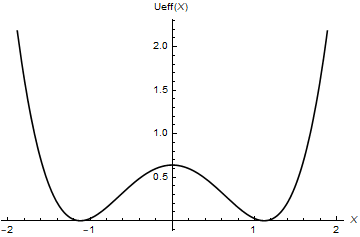
\includegraphics[scale=.7]{imagenes/sech-aprox.png}
    \caption{Forma de referencia del potencial efectivo para el caso de estudio $\epsilon=0.8$,$\gamma=0.64$ }.
    \label{fig:9.1}
\end{figure}

A partir de la forma del potencial efectivo se obtienen los puntos de equilibrio estable e inestables para el electrón, se encuentra que este efectuará oscilaciones alrededor de alguno de los puntos de equilibrio estable $X=\pm \sqrt{\epsilon/\gamma}$, con frecuencia de pequeñas oscilaciones:

\begin{equation}\label{eq:9.39}
    \omega_1=\frac{\sqrt{\gamma\epsilon}}{ m^*\omega}
\end{equation}

Se encuentran un punto de equilibrio inestable en $X=0$, y dos puntos de equilibrio estable en:

\begin{equation}\label{eq:9.40}
    X=\pm \sqrt{\frac{\epsilon}{\gamma}}
\end{equation}

Se ha hecho un diagrama de fases que permite observar de forma referencial, la evolución de la velocidad en función de la posición del electrón para distintas velocidades iniciales. Se puede observar que para velocidades iniciales pequeñas y en las cercanías de los puntos de equilibrio estable el electrón experimenta ciclos cerrados en el diagrama de fases, lo cual indica la presencia de oscilaciones alrededor de dichos puntos. Además se observa que para velocidades suficientemente grandes, el electrón realiza oscilaciones alrededor de $x=0$ pasando por los puntos de equilibrio estable e inestable en cada oscilación.

\begin{figure}[H]
    \centering
    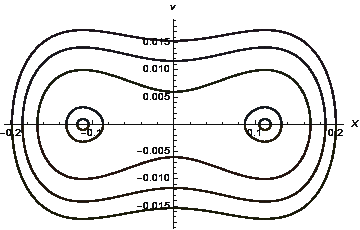
\includegraphics[scale=1]{imagenes/fase-clasico2.png}
    \caption{Diagrama de velocidad en función de la posición,$\epsilon=0.8$, $\gamma=0.64$, $\omega=100$ }
    \label{fig:9.2}
\end{figure}

\chapter{Método de Floquet-Magnus aplicado al cálculo de Hamiltonianos efectivos}\label{cap:10}

En esta sección se desarrolla un método para describir la dinámica cuántica del electrón en la red, bajo la influencia de campos externos rápidamente oscilantes. Se utilizan métodos perturbativos, en especifico, la ya estudiada expansión de Floquet-Magnus. Se calculan los Hamiltonianos efectivos y sus respectivas energías y autofunciones para los casos de perturbación lineal y no lineal dependientes del tiempo. 

La dinámica de una partícula cuántica esta descrita por la ecuación de Schrödinger:

\begin{equation}\label{eq:10.1}
    i\hbar\frac{\partial \Psi(x,t)}{\partial t}=H(x,t)\Psi(x,t)
\end{equation}

Donde se observa que el Hamiltoniano del electrón es una función dependiente del tiempo. Se conoce la forma de las soluciones a esta ecuación diferencial gracias a la Teoría de Floquet, y se usa la expansión de Floquet-Magnus, la cual se desarrolló en el capítulo \ref{cap:8}. Se va a aplicar este método sobre Hamiltonianos que tienen la forma general presentada en la siguiente ecuación: 

\begin{equation}\label{eq:10.2}
    H(x,t)=-2A\cos(ak)+V_1(x)+V_2(x,t)
\end{equation}

Este es el hamiltoniano para un electrón en una red de \textit{Enlace Fuerte}, a la cual se ha agregado una perturbación independiente del tiempo $V_1(x)$ y una perturbación rápidamente oscilante de frecuencia $\omega \gg \omega_0$, donde $\omega_0$ es la frecuencia de las oscilaciones de Bloch.

La solución a la ecuación de Schrödinger para el Hamiltoniano de estudio fue dada por Floquet y tiene la forma:

\begin{equation}\label{eq:10.3}
    \Psi(\rho,t)=P(t)e^{-i\overline{H}t}\psi(\rho)
\end{equation}

%\begin{equation}\label{eq:10.4}
 %   \psi(\rho,t)=\sum^{\infty}_{n=-\infty} b_n e^{i(an+\lambda)\rho}
%\end{equation}

Las fórmulas recursivas de Floquet-Magnus permiten hallar el hamiltoniano efectivo para el sistema que se desea estudiar. Las fórmulas están por: 

\begin{equation}\label{eq:10.5}
    G^{(k)}=\frac{1}{T}\int^{T}_{0}\{ H(t')P^{(k-1)}(t')-\sum^{k-1}_{j=1} P^{(j)}G^{(k-j)}\}dt'
\end{equation}

\begin{equation}\label{eq:10.6}
    P^{(k)}=-i\int^{t}_{0}\{ H(t')P^{(k-1)}(t')-\sum^{k-1}_{j=1} P^{(j)}G^{(k-j)}-G^{(k)}\}dt'
\end{equation}

Los términos de orden cero en las ecuaciones \ref{eq:10.5} y \ref{eq:10.6} se han definido como en las ecuaciones \ref{eq:10.7} y \ref{eq:10.8}, tal y como se hizo en el capítulo \ref{cap:8}:

\begin{equation}\label{eq:10.7}
    \begin{cases}
        G^{(0)}=0\\
        P^{(0)}=1
    \end{cases}
\end{equation}

\begin{equation}\label{eq:10.8}
\begin{cases}
    G=\sum G^{(k)}\\
    P=\sum P^{(k)}
    \end{cases}
\end{equation}

Donde $\overline{H}=G$. Para este trabajo especial de grado se estudian las perturbaciones dependientes del tiempo que tienen la siguiente forma general:

\begin{equation}\label{eq:10.9}
    V_2(x,t)=V(x)\cos(\omega t)
\end{equation}

Para efectos del calculo de $P^{(k)}$ y $G^{(k)}$ se ha creado un programa en \textit{Mathematica} cuyo algoritmo permite el cálculo hasta orden $k=5$ para cualquier perturbación externa del electrón en la red. 

\section{Dinámica del electrón en la red de \textit{Tight Binding} en presencia de una perturbación lineal dependiente del tiempo }

En esta sección se estudia el caso del electrón en la red de \textit{Tight Binding}, en presencia de un potencial eléctrico externo lineal y rápidamente oscilante. El Hamiltoniano de este sistema tiene la siguiente forma:

\begin{equation}\label{eq:10.10}
    H(x,t)=2A\cos(a\rho)+\epsilon x \cos(\omega t)
\end{equation}

Haciendo uso de la expansión de Floquet-Magnus se calculan los $G^{(k)}$ hasta $k=5$ y los $P^{(k)}$ hasta $k=4$ con ayuda del programa de \textit{Mathematica} hecho especialmente para este fin. A continuación se presentan los resultados obtenidos:

\subsection{Cálculo de los $G_{(K)}$ y $P_{(k)}$}

\begin{equation}\label{eq:10.11}
    G^{(1)}=-2A\cos(ap)=H_o
\end{equation}

\begin{equation}\label{eq:10.12}
    P^{(1)}=\frac{\epsilon\sin(\omega t)}{\omega}\mathbb{I}
\end{equation}

\begin{equation}\label{eq:10.13}
    G^{2}=0
\end{equation}

\begin{equation}\label{eq:10.14}
    P^{(2)}=\frac{\epsilon\sin^2(\frac{t\omega}{2})}{\omega^2}[4iaA\sin(ap)\mathbb{I}+2\epsilon\cos^2(\frac{t\omega}{2})\frac{\partial^2}{\partial p^2}]
\end{equation}

\begin{equation}\label{eq:10.15}
    G^{(3)}=\frac{a^2A\epsilon^2\cos(ap)}{2\omega^2}\mathbb{I}
\end{equation}

\begin{equation}\label{eq:10.16}
         \begin{split}         P^{(3)}=&\frac{\epsilon^2}{12\omega^3}[3ia^2A(8\sin(\omega t)-3\sin(2\omega t))\cos(ap)\mathbb{I} +\\&+48iaA\sin^2(\frac{\omega t}{2})\sin(\omega t)\sin(ap)\frac{\partial}{\partial p}+\\&+ 2i\epsilon\sin^3(\omega t)\frac{\partial^3}{\partial p^3}]
    \end{split}
\end{equation}

\begin{equation}
  G^{(4)}=0  
\end{equation}

\begin{equation}\label{eq:10.17}
\begin{aligned}
        &P^{(4)}=\frac{\epsilon^2 \sin ^2\left(\frac{t \omega}{2}\right)}{36 \omega^4} (6 \epsilon^2  \sin ^2(t\omega) \cos^2 \left(\frac{t \omega}{2}\right)\frac{\partial^4}{\partial p^4}-\\&-72 i a^2 A \epsilon  \cos (a p) \cos
   ^2\left(\frac{t \omega}{2}\right) (3 \cos (t \omega)-4)\frac{\partial}{\partial p}+\\&+72 i a A \epsilon \sin (a p) \sin ^2(t \omega)\frac{\partial^2}{\partial p^2}-\\&-2 i a^2 A \sin (a p) (a \epsilon (14 \cos (t w)-11 \cos (2 t \omega)+33)+\\&+72 i A \sin (a p) (\cos
   (t \omega)-1))\mathbb{I})
    \end{aligned}
\end{equation}

\begin{equation}\label{eq:10.18}
    G^{(5)}=-\frac{a^4 A \epsilon^4\cos(a p)}{32 \omega^4}\mathbb{I}
\end{equation}


 Estos resultados fueron contrastados con los de Martínez et al.(2017) obteniendo exactamente las mismas expresiones para los $G$ y $P$ hasta $k=5$ \cite{martinez2017}. Al observar con detenimiento las expresiones para $G^{(k)}$ en $k=1,2,3,4,5$ se observa que es posible encontrar una solución general para cualquier  $G^{(k)}$,

\begin{equation}\label{eq:10.19}
    G^{[1]} \approx G^{(0)}+G^{(1)}=-2A\cos (a p)\mathbb{I}
\end{equation}

\begin{equation}\label{eq:10.20}
    G^{[3]} \approx G^{(0)}+G^{(1)}+G^{(2)}+G^{(3)}=-2A\cos (a p)\left(1-\frac{a^2 \epsilon^2  }{4 \omega^2}\right)\mathbb{I}
\end{equation}

\begin{equation}\label{eq:10.21}
    G^{[5]} \approx G^{(0)}+G^{(1)}+G^{(2)}+G^{(3)}+G^{(4)}+G^{(5)}=-2A\cos (a p)\left(1-\frac{a^2 \epsilon^2  }{4 \omega^2}+\frac{a^4 \epsilon^4}{64 \omega^4}\right)\mathbb{I}
\end{equation}

\begin{equation*}
    \vdots
\end{equation*}

\begin{equation}\label{eq:10.22}
    G^{[n+1]} \ \ \overrightarrow{n \rightarrow \infty} \ \
 G^{(0)}+G^{(1)}+\dots G^{n+1}=-2A\cos(a p)\mathcal{J}_0(\frac{\omega_B}{\omega})\mathbb{I}
\end{equation}

La ecuación \ref{eq:10.22} es el resultado de la convergencia de $G$ para el caso que se está estudiando, donde $\mathcal{J}_0(z)$ es la función de Bessel, definida como:

\begin{equation}\label{eq:10.23}
    \mathcal{J}_0(z)=\sum^{\infty}_{m=0}\frac{(-1)^m}{(m!)^2}(\frac{z}{2})^{2m}
\end{equation}

Este resultado coincide con los resultados de Dunlap y Kenkre \cite{Dunlap} para el electrón en campos eléctricos oscilantes. En su artículo de 1984, ellos hallaron que el electrón moviéndose en campos eléctricos oscilantes, tiene un potencial y Hamiltoniano efectivo de la forma siguiente:

\begin{equation}
    H(X,K)=H_0(X,K)\mathcal{J}_0(\omega_0/\omega)
\end{equation}

\begin{equation}
U_{eff}(X)=U(X)\mathcal{J}_0(\omega_0/\omega)    
\end{equation}

Donde $\mathcal{J}_0(\omega_0/\omega)$ es la función de Bessel a orden cero. Estas ecuaciones indican la presencia del fenómeno de \textit{Band Narrowing}. En los puntos donde se anula la función $\mathcal{J}_0$ de Bessel la banda de energía y la interacción efectiva entre el electrón y la red se anulan. Se observa además que el campo externo oscilante tiene el efecto de reducir la velocidad efectiva o de deslocalización del electrón inicialmente localizado \cite{Dunlap}.

 Se obtienen las funciones de onda del electrón según la Teoría de Floquet-Magnus:

\begin{equation}\label{eq:10.24}
\begin{split}
    \Psi(t,p)&=P(t)e^{i\overline{H}t}\psi(p)
    \\&=CP(t)e^{iE(p)t}\delta(p-p')
\end{split}
\end{equation}

Donde $\psi(p)=C\delta(p-p')$ es la autofunción generalizada de $G$ y $E(p)=-2A\cos(a p)\mathcal{J}_0(\frac{\omega_B}{\omega})$ es su autovalor generalizado. Se aproxima la $P(t)$ y $G$ hasta orden de $\omega^{-2}$:

\begin{equation}\label{eq:10.25}
    G \approx -2A\cos (a p)\mathcal{J}
\end{equation}

\begin{equation}
    \mathcal{J}=1-\frac{a^2 \epsilon^2  }{4 \omega^2}
\end{equation}

\begin{equation}\label{eq:10.26}
    P(t)=\left(1+\frac{\epsilon\sin(\omega t)}{\omega}+\frac{4iaA\epsilon\sin^2(\frac{t\omega}{2})\sin(ap)}{\omega^2}\right)\mathbb{I}+\frac{\epsilon^2}{\omega^2}\sin^2(t\omega)\frac{\partial^2}{\partial p^2}
\end{equation}
 
 Se escoge la solución:
 
 \begin{equation}\label{eq:10.27}
     \psi(p)=\frac{a}{2\pi}\sum^{\infty}_{-\infty} e^{in(p-p')a}
 \end{equation}
 
Entonces se puede calcular la posición cuadrática promedio, y se obtiene la siguiente expresión:

\begin{equation}\label{eq:10.28}
    \bra{\Psi}X^2\ket{\Psi}\approx 2A^2a^2\mathcal{J}^2(\frac{\omega_B}{\omega})t^2
\end{equation}

Se observa que por efecto de la fuerza oscilante externa, la partícula se deslocaliza de su punto de origen y no efectúa movimientos oscilatorios. Se encuentra que este resultado coincide con el estudio semiclásico que se hizo previamente de este mismo sistema, donde el electrón también resultaba no localizado.

\section{Dinámica del electrón en la red de Enlace Fuerte en presencia de una perturbación no lineal dependiente del tiempo}

En este segundo caso de estudio se trabaja con una perturbación no lineal dependiente del tiempo, en particular la tangente hiperbólica multiplicada por $\cos(\omega t)$. En este caso el Hamiltoniano tiene la siguiente forma:

\begin{equation}\label{eq:10.29}
    H(x,t)=2A\cos(a\rho)+\tanh(\alpha x)\cos(\omega t)
\end{equation}

La perturbación, cuya inhomogeneidad en el espacio tiene la forma referencial dada por la figura \ref{fig:10.1}, tiene cierta similitud con la  ya estudiada por Martínez et al. \cite{martinez2017}, donde se estudió la inhomogeneidad lineal multiplicada por una función rápidamente oscilante. La diferencia que destaca en nuestro caso, es que, a diferencia de una perturbación lineal, la tangente hiperbólica tiene límites finitos cuando se hace tender a infinito y menos infinito, característica que la hace más realista, si a sentido físico se refiere, ya que la linealidad se limita a una región del espacio finito, mientras que en las zonas alejadas del origen la tangente está acotada con pendiente casi nula, por lo que en estas zonas el electrón experimenta fuerzas despreciables.


\begin{figure}[H]
    \centering
    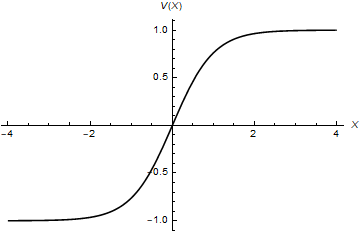
\includegraphics{imagenes/potencial_oscilante.png}
    \caption{Forma referencial de la inhomogeneidad $V(x)=\tanh(x)$}
    \label{fig:10.1}
\end{figure}

En lo sucesivo, se necesita tratar la inhomogeneidad como un operador cuántico. Se expande la $\tanh(\epsilon x)\approx \epsilon x - \gamma\frac{x^3}{3}$ y se sustituye $x$ por el operador de posición $x=i\frac{d}{d\rho}$. De esta manera el Hamiltoniano tiene la forma:

\begin{equation}\label{eq:10.30}
    \hat{H}(x,t)=2A\cos(a\rho)\mathbb{I}+i\cos(\omega t)\left( \epsilon \frac{\partial}{\partial \rho} + \frac{\gamma}{3}\frac{\partial^3}{\partial \rho^3}\right)
\end{equation}

Se hizo uso del programa en \textit{Mathematica} (ap\'endice \ref{apendice:E}) especialmente desarrollado para este cálculo y se obtuvo los siguientes resultados para los $G^k$ y $P^k$ (Esto se hizo hasta orden $k=3$ y tomando $\gamma^2=0$).

\subsection{Cálculo de $G_{(k)}$ y $P_{(k)}$}

\begin{equation}\label{eq:10.31}
    \hat{G}^{1}=-2 A \cos(a p)\mathbb{I}
\end{equation}

\begin{equation}\label{eq:10.32}
    \hat{P}^{1}=\frac{\sin(\omega t)}{3 \omega} \left(3 \epsilon \frac{\partial}{\partial \rho}+\gamma \frac{\partial^3}{\partial \rho^3}\right)
\end{equation}

\begin{equation}\label{eq:10.33}
    \hat{G}^{2}=0
\end{equation}

\begin{equation}\label{eq:10.34}
\begin{split}
     \hat{P}^{2}=&4iaA\frac{\sin (a \rho) \sin ^2\left(\frac{t \omega}{2}\right)}{\omega^2}\left( \epsilon-\frac{
    a^2 \gamma }{3}\right)\mathbb{I}+\left(\frac{4 i a^2 A \gamma }{\omega^2}\cos (a \rho) \sin ^2\left(\frac{\omega t}{2}\right)\right)\frac{\partial}{\partial \rho}+\\
    &+\frac{\sin ^2\left(\frac{t w}{2}\right)}{w^2}\left[\epsilon^2\left(1 +\cos (\omega t)\right)+4 i a A l \sin (a \rho) \right]\frac{\partial^2}{\partial \rho^2}+\frac{\epsilon \gamma \sin ^2(\omega t)}{3 \omega^4}\frac{\partial^4}{\partial \rho^4}
 \end{split}
\end{equation}

\begin{equation}\label{eq:10.35}
\begin{split}
    &\hat{G}^{3}=\frac{a^2 A\cos (a \rho)}{\omega^2}\left(\frac{ \epsilon^2 }{2}-\frac{\left(\gamma a^2
   \epsilon+24 i\gamma aA \sin (a \rho)\right)}{3 }\right)\mathbb{I}+\\&
   -\left(\frac{\gamma a^2A \sin (a \rho)}{\omega^2}\left(a \epsilon+8 i A \sin (a \rho)\right)\right)\frac{\partial}{\partial \rho}+\frac{a^2 A \epsilon \gamma \cos (a \rho)}{\omega^2}\frac{\partial^2}{\partial \rho^2}
\end{split}
\end{equation}

\subsection{Cálculo del Hamiltoniano efectivo y el operador de micromovimiento}

\begin{equation}\label{eq:10.36}
\begin{split}
     &\overline{H}=A\cos (a \rho)\left(\frac{ \epsilon^2a^2 }{2 \omega^2}-\frac{\left(\gamma a^4
   \epsilon+24 i a^3 A\gamma \sin (a \rho)\right)}{3 \omega^2}-2 \right)\mathbb{I}+\\&
   -\left(\frac{\gamma a^2A \sin (a \rho)}{\omega^2}\left(a \epsilon+8 i A \sin (a \rho)\right)\right)\frac{\partial}{\partial \rho}+\frac{a^2 A \epsilon \gamma \cos (a \rho)}{\omega^2}\frac{\partial^2}{\partial \rho^2}
   \end{split}
\end{equation}

\begin{equation}\label{eq:10.37}
    \begin{split}
        &P=\left(1+\frac{4 iAa\sin (a p) \sin ^2\left(\frac{\omega t}{2}\right)}{\omega ^2}\left(-\frac{ a^2 \gamma }{3}+  \epsilon\right)\right)+
   \\&+\left(\frac{\epsilon \sin (\omega t)}{\omega}+\frac{4 i a^2 A \gamma \cos (a \rho) \sin ^2\left(\frac{\omega t }{2}\right)}{\omega^2}\right)\frac{\partial}{\partial \rho}+\\&+
   \frac{1}{\omega^2}\left(4 i a A \gamma \sin (a \rho)\sin ^2\left(\frac{\omega t }{2}\right) +\frac{\epsilon^2}{2} \sin^2 (\omega t )\right)\frac{\partial^2}{\partial \rho^2}+
   \\&+\frac{\gamma \sin (\omega t)}{3 \omega}\frac{\partial^3}{\partial \rho^3}+\frac{\epsilon \gamma \sin ^2(\gamma t)}{3 \omega^2}\frac{\partial^4}{\partial \rho^4}
    \end{split}
\end{equation}

En el espacio real, el Hamiltoniano efectivo toma la forma de la siguiente ecuación, se observa que la energía, en ausencia de la perturbación dependiente del tiempo presenta dependencia únicamente del momento, y en presencia de la perturbación dependiente del tiempo va a depender del momento y la posición $x$.

\begin{equation}\label{eq:10.36.6}
\begin{split}
     &\overline{H}=-2A\cos (a \rho)\left(1-\frac{ \epsilon^2a^2 }{4 \omega^2}+\frac{\left(\gamma a^4
   \epsilon+24 i a^3 A\gamma \sin (a \rho)\right)}{6 \omega^2} \right)+\\&
   -\left(\frac{\gamma a^2A \sin (a \rho)}{\omega^2}\left(a \epsilon+8 i A \sin (a \rho)\right)\right)x+\frac{a^2 A \epsilon \gamma \cos (a \rho)}{\omega^2}x^2
   \end{split}
\end{equation}

\subsection{Obtención de la ecuación de Schrödinger}

La ecuación de Schrödinger independiente del tiempo es: 

\begin{equation}\label{eq:10.38}
    \overline{H}\psi(\rho)=E(\rho)\psi(\rho)
\end{equation}

Una vez obtenida una expresión para la ecuación de Schrödinger independiente del tiempo, se quiere calcular las autoenergías y autofunciones del electrón en el sistema de estudio. Para lograr esto se hace uso de la teoría de ecuaciones diferenciales de Hill.

De \ref{eq:10.36} se observa que la ecuación de Schrödinger tiene la siguiente forma:

\begin{equation}\label{eq:10.39}
\begin{split}
     &-2A\cos (a \rho)\left(1-\frac{ \epsilon^2a^2 }{4 \omega^2}+\frac{\left(\gamma a^4
   \epsilon+24 i a^3 A\gamma \sin (a \rho)\right)}{6 \omega^2} \right)\psi(\rho)+\\&
   -\left(\frac{\gamma a^2A \sin (a \rho)}{\omega^2}\left(a \epsilon+8 i A \sin (a \rho)\right)\right)\frac{\partial}{\partial \rho}\psi(\rho)+\frac{a^2 A \epsilon \gamma \cos (a \rho)}{\omega^2}\frac{\partial^2}{\partial \rho^2}\psi(\rho)=E(\rho)\psi(\rho)
   \end{split}
\end{equation}

A hacer la substitución $\gamma=0$ se vuelve a obtener el resultado para la perturbación lineal dependiente del tiempo a orden $\omega^{-2}$. La ecuación \ref{eq:10.39} puede reducirse a la siguiente ecuación diferencial: 

\begin{equation}\label{eq:10.40}
    f''(\rho)+\left(\frac{A^2a^2\epsilon\gamma}{\omega^2}+\frac{A^2a^2\epsilon\gamma}{\omega^2}\cos(2a\rho)+\frac{E(\rho)a^2A\epsilon\gamma}{\omega^2}\cos(a\rho)\right) f(\rho)=0
\end{equation}


Esta última ecuación, es una ecuación de Hill de la forma:

\begin{equation}\label{eq:10.41}
    u''+(\theta_0+2\theta_1\cos(a\rho)+2\theta_2\cos(2a\rho))u=0
\end{equation}

Donde los valores de $\theta_i$ son los siguientes:

\begin{equation}\label{eq:10.42}
    \theta_2=\frac{A^2a^2\epsilon\gamma}{2\omega^2}
\end{equation}

\begin{equation}\label{eq:10.43}
    \theta_1=\frac{Ea^2A\epsilon\gamma}{2\omega^2}
\end{equation}

\begin{equation}\label{eq:10.44}
\begin{split}
       &\theta_0=\frac{A^2a^2\epsilon\gamma}{\omega^2}
\end{split}
\end{equation}

Para que la solución sea no trivial, se sabe de la teoría de ecuaciones de Hill que debe cumplirse la siguiente relación para \ref{eq:10.41}, esta condición garantiza que las soluciones a la ecuación diferencial de Hill sean no triviales (u=0): 

\begin{equation}\label{eq:10.45}
\Delta_{(0)}\sin^2(\frac{\pi}{a}\theta_o^{1/2})=\sin^2(\pi\lambda)
\end{equation}

Donde $\Delta(0)$ en el determinante infinito de Hill, esta matriz se trunca a una de tamaño $3 \times 3$ basado en la rápida convergencia de la solución de las ecuaciones diferenciales de Hill. 

\large
\begin{equation}\label{eq:10.46}
\Delta(0)^1=
\begin{vmatrix}
 & 1 & \frac{\theta_1}{\theta_o-a^2} & \frac{\theta_2}{\theta_0-a^2} & \\[0.3cm] 
 & \frac{\theta_1}{\theta_o} & 1 & \frac{\theta_1}{\theta_o} &  \\[0.3cm]
 & \frac{\theta_2}{\theta_0-a^2} & \frac{\theta_1}{\theta_o-a^2} & 1 &  \\[0.3cm] 
\end{vmatrix}=0
\end{equation}
\normalsize

El calculo de este determinante lleva a la siguiente ecuación, de la cual se pueden despejar los valores de las autoenergías permitidas para este sistema: 

\begin{equation}\label{eq:10.47}
    \Delta(0)^1\approx1+\frac{2\theta_1^2\theta_2-\theta_2^2\theta_0-2\theta_1^2(\theta_0-a^2)}{\theta_0(\theta_0-a^2)^2}
\end{equation}

Se hace la aproximación $\theta_0\approx 0$ y $\lambda$ se supone entero, entonces:

\begin{equation}\label{eq:10.48}
\left(1+\frac{2\theta_1^2\theta_2-\theta_2^2\theta_0-2\theta_1^2(\theta_0-a^2)}{\theta_0(\theta_0-a^2)^2}\right)\frac{\pi^2}{a^2}\theta_0=0
\end{equation}

Realizando operaciones algebraicas y sustituyendo \ref{eq:10.42}, \ref{eq:10.43}, \ref{eq:10.44} sobre \ref{eq:10.48} se obtienen las autoenergías del electrón en el sistema de estudio: 

\begin{equation}\label{eq:10.49}
   E=\pm \frac{\sqrt{3 A^2 \epsilon \gamma-2 \omega^2}}{\sqrt{\epsilon\gamma}}
\end{equation}

\begin{figure}[H]
    \centering
    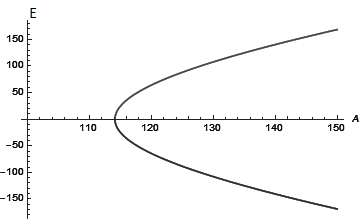
\includegraphics[scale=1]{imagenes/esp-energia.png}
    \caption{Energía del electrón en función del parámetro de energías del electrón A, $\epsilon=0.8$, $\gamma=0.64$, $\omega=100$}
    \label{fig:10.2}
\end{figure}

\begin{figure}[H]
    \centering
    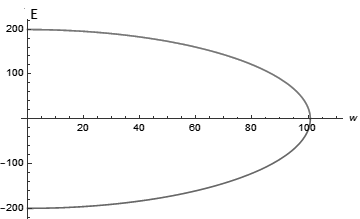
\includegraphics[scale=.8]{imagenes/ener-w.png}
    \caption{Energía del electrón en función de la frecuencia forzante $\omega$, $\epsilon=0.8$, $\gamma=0.64$, $A=115$}
    \label{fig:10.3}
\end{figure}

\begin{figure}[H]
    \centering
    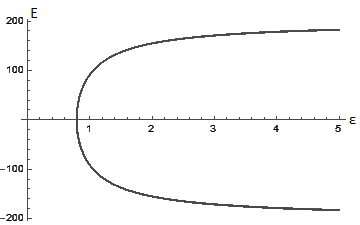
\includegraphics[scale=1]{imagenes/ener-e.png}
    \caption{Energía del electrón en función del parámetro $\epsilon$, $\omega=100$, $\gamma=0.64$, $A=115$}
    \label{fig:10.4}
\end{figure}

Se observa que la condición para estabilidad de las soluciones junto con la condición de no trivialidad ocasionan que la energía este limitada para ciertos valores de $A$, $\epsilon$ y $\omega$.

\subsection{Cálculo de las autofunciones}

Se calculan ahora las autofunciones del electrón, recordando las soluciones a las ecuaciones de Hill, se tiene que las soluciones de \ref{eq:10.40} tienen la forma:

\begin{equation}\label{eq:10.50}
    \psi(\rho)=\sum^{\infty}_{n=-\infty} b_n e^{i(an+\lambda)\rho}
\end{equation}

Además de la teoría de la expansión de Floquet-Magnus, las autofunciones del electrón estarán dadas por:

\begin{equation}\label{eq:10.51}
    \Psi(t,p)=P(t)e^{i\overline{H}t}\psi(p)
\end{equation}

Haciendo uso de \ref{eq:10.50} y \ref{eq:10.51} se obtiene la forma de la función de onda del electrón en el sistema.

\small
\begin{equation}\label{eq:10.52}
    \begin{split}
    &\Psi(\rho,t)=e^{-iEt}\sum^{\infty}_{n=-\infty}b_n\frac{e^{i \rho (a n+\lambda)}}{12 \omega^2} (-4 i (\omega (a n+\lambda) \sin (t \omega) \left(\gamma (a n+\lambda)^2-3 \epsilon\right)+\\&+4 a A \sin
   ^2\left(\frac{t \omega}{2}\right) \left(\sin (a \rho) \left(\gamma \left(3 a^2 n^2+a^2+6 a n \lambda+3 \lambda^2\right)-3 \epsilon\right)-3 i
   a \gamma (a n+\lambda) \cos (a \rho)\right))+\\&+\epsilon (a n+\lambda)^2 \cos (2 t \omega) \left(3 \epsilon-2 \gamma (a
   n+\lambda)^2\right)+\epsilon (a n+\lambda)^2 \left(2 \gamma (a n+\lambda)^2-3 \epsilon\right)+12 \omega^2)
   \end{split}
\end{equation}

\normalsize
Teniendo la forma de las autofunciones es posible hacer un estudio de la dinámica del electrón en el sistema de estudio y evaluar el comportamiento de las densidades de probabilidad en el espacio real y recíproco. De tal manera que es posible conocer la posición del electrón en el espacio de momentos y el espacio real para distintos espacios temporales. 

\begin{figure}[H]
    \centering
    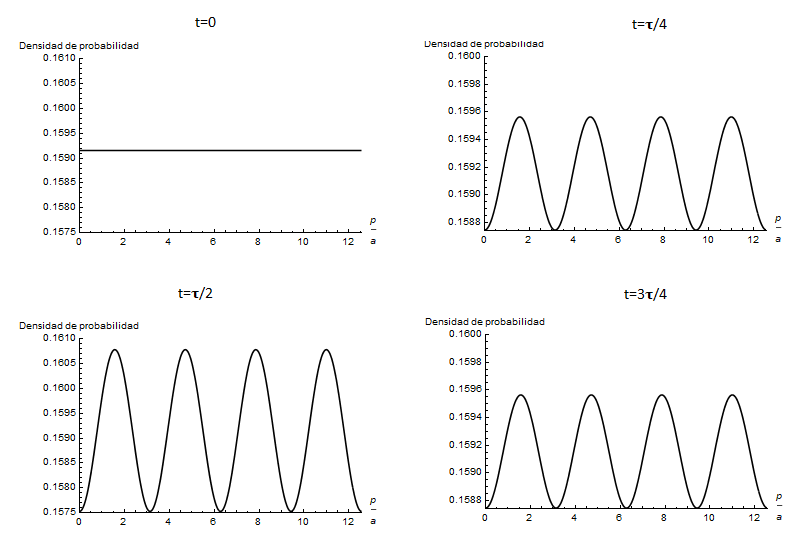
\includegraphics[width=1\columnwidth]{imagenes/dens_prop_pt0.png}
    \caption{Densidad de probabilidad en el espacio reciproco en función del momento en distintos $t$ que están dentro de un periodo de oscilación rápida $\tau=2\pi/\omega$, $\omega=50$, $a=0.1$, $A=1000$, $\epsilon=0.9$, $\gamma=0.81$}
    \label{fig5.11}
\end{figure}

Se observa que existe una periodicidad en el comportamiento de la densidad de probabilidad en el espacio de momentos $\rho$, con periodo $\tau=2\pi/\omega$. Durante este periodo la densidad de probabilidad pasa de tener una frecuencia nula a tener una frecuencia bien definida, con aumentos y disminución de la intensidad periódicos. Esto indica que en todo momento el electrón tiene una frecuencia de onda en el espacio recíproco constante, por lo que se espera que en el espacio real el electrón se encuentre bien localizado. 

\begin{figure}[H]
    \centering
    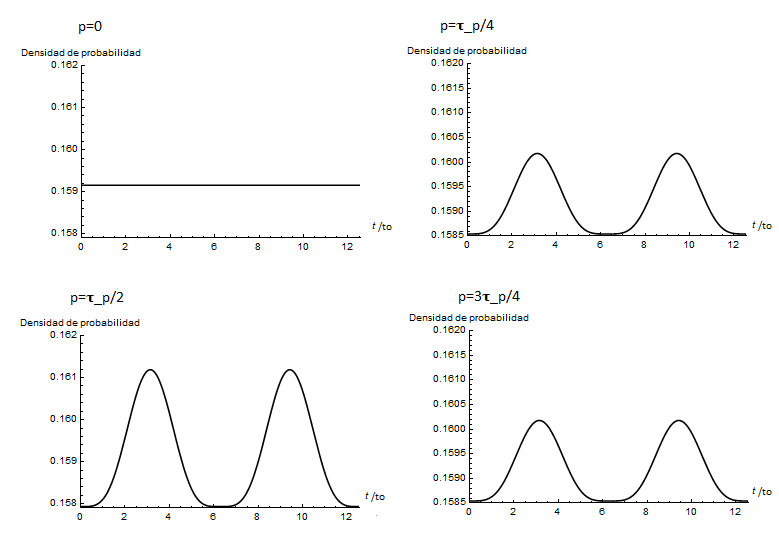
\includegraphics[width=1\columnwidth]{imagenes/dens_prop_tp1.png}
    \caption{Densidad de probabilidad en el espacio rec\'iproco en función del tiempo para distintos $\rho$ que están dentro de un periodo $\tau_{\rho}=2\pi/a$, $\omega=50$, $a=0.1$, $A=1000$, $\epsilon=0.9$, $\gamma=0.81$}
    \label{fig10.6}
\end{figure}

Una mirada al comportamiento de la densidad de probabilidad del electrón en el espacio recíproco en función del tiempo para distintos $\rho$, indica que para momento nulo o múltiplos de un periodo la densidad de probabilidad del electrón permanece constante, mientras que para momentos que están dentro del intervalo abierto $(0,2\pi/a)$  la densidad de probabilidad experimentará oscilaciones de frecuencia constante.  

Calculando la transformada de Fourier de la función de onda encontrada para el electrón, es posible obtener la expresión para la función de onda del electrón en el espacio real. A partir de ésta se halló la densidad de probabilidad y se han realizado los siguientes gráficos de densidad de probabilidad en el espacio real en distintos tiempos, para tiempos que están dentro del periodo $\tau=2\pi/\omega$. 

\begin{figure}[H]
    \centering
    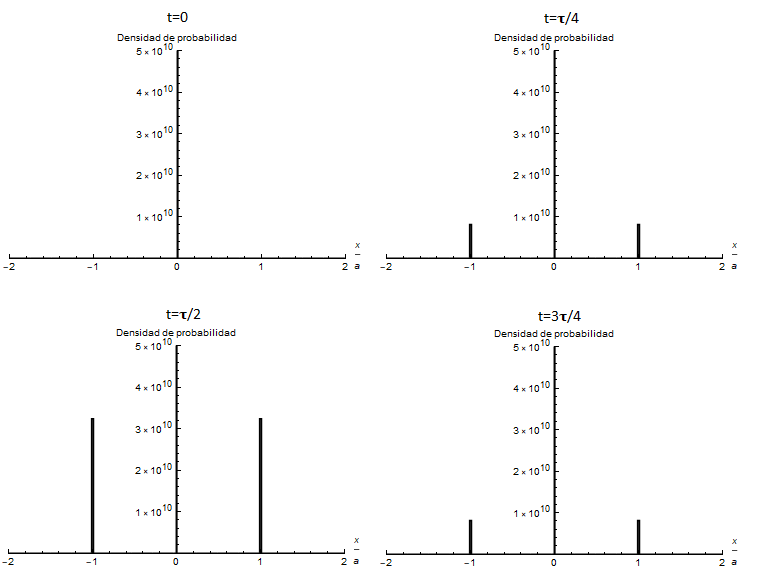
\includegraphics[width=1\columnwidth]{imagenes/dens_prop_tx.png}
    \caption{Densidad de probabilidad en el espacio real para distintos $t$, en un periodo $\tau=2\pi/\omega$, $\omega=50$, $a=0.1$, $A=1000$, $\epsilon=0.9$, $\gamma=0.81$}
    \label{fig5.13}
\end{figure}

Se encuentra que la posición del electrón en el espacio real se encuentra bien definida como deltas de Dirac. En $t=0$ o múltiplos del periodo, el electrón estará totalmente localizado en $x=0$, para tiempos intermedios el electrón tendrá tres posibles puntos de localización simétricos con el eje de las ordenadas. 

Una de las condiciones para afirmar la existencia de la localización dinámica del electrón, es que el valor esperado de la posición cuadrática esté acotada para todo tiempo. Al calcularlo se ha podido determinar que el valor esperado de la posición cuadrática es en efecto periódica y acotada para todo tiempo t. El siguiente gráfico muestra la forma resultante de la función que se obtuvo.

\begin{figure}[H]
    \centering
    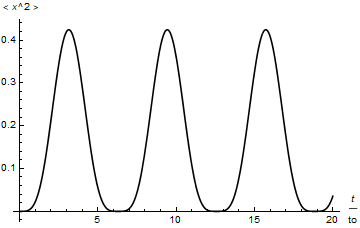
\includegraphics[scale=.7]{imagenes/x2-prom.png}
    \caption{Valor esperado de la posición al cuadrado en función del tiempo,$\omega=50$, $a=0.1$, $A=1000$, $\epsilon=0.9$, $\gamma=0.81$,$t_0=0,02$}
    \label{fig:5.14}
\end{figure}

De igual manera se ha calculado el valor esperado del momento cuadrado, se ha encontrado que este también es acotado y periódico, con valores que van desde cero asta un valor máximo, esto es evidencia de un comportamiento oscilatorio del electrón en el sistema de estudio. El siguiente gráfico muestra el comportamiento antes mencionado.

\begin{figure}[H]
    \centering
    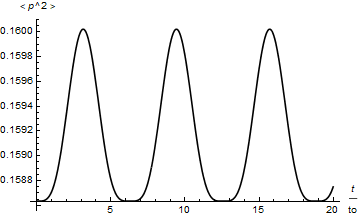
\includegraphics[scale=.7]{imagenes/p2-prom.png}
    \caption{Valor esperado del momentum al cuadrado en función del tiempo, $\omega=50$, $a=0.1$, $A=1000$, $\epsilon=0.9$, $\gamma=0.81$,$t_0=0,02$}
    \label{fig:5.15}
\end{figure}

Finalmente se ha calculado el valor esperado de momento y la posición del electrón, encontrándose que ambos tienen valor cero, lo cual confirma, junto con los otros resultados encontrados, que el electrón presenta el fenómeno de localización dinámica en el sistema de estudio.
\begin{equation}
    \begin{cases}
    \overline{x}=0\\ 
    \overline{p}=0
    \end{cases}
\end{equation}

\chapter*{Conclusiones}

 Se modeló la dinámica de un electrón en una red unidimensional, cuando sobre él actúan campos eléctricos externos inhomogéneos y rápidamente oscilantes, usando el modelo de \textit{Tight Binding}. La red utilizada es periódica, homonuclear, sin impurezas y restringiendo al electrón a mantenerse dentro de una sola banda. 
Se hizo uso del modelo semiclásico y el método de Kapitza para encontrar el potencial efectivo del electrón y de la teoría de Floquet y la expansión de Floquet-Magnus para obtener los  Hamiltonianos efectivos cuánticos logrando reproducir los resultados de Martínez et al. (2017) \cite{martinez2017} y Martínez et al. (2014) \cite{mart2014}, este último con una modificación en el orden de aproximación. 

Haciendo uso del enfoque semiclásico, se obtuvieron la forma del potencial efectivo, el Hamiltoniano efectivo y la masa efectiva del electrón; lo que permitió obtener un modelo para la dinámica en la red de \textit{Tight Binding} bajo la influencia de cualquier potencial externo, rápidamente oscilante o no. Se halló que en límite del continuo el potencial efectivo, el Hamiltoniano efectivo y la masa efectiva tienden al los resultados de Kapitza \cite{kapitza}, Landau \cite{landau} y Malay Bandyopadhyay et al. \cite{datta}.

Los resultados obtenidos fueron utilizados para modelar la dinámica del electrón en presencia de un potencial externo lineal y otro tipo tangente hiperbólica, ambos rápidamente oscilantes. Obteniendo que para el potencial lineal el electrón no presenta comportamiento oscilatorio, por ende, el electrón tendrá una dinámica con posición no acotada. En el caso de la tangente hiperbólica se halló que el potencial efectivo tiene dos puntos de equilibrio estable simétricos con el origen y uno inestable en el origen. Para los puntos de equilibrio estables se calculó la frecuencia de pequeñas oscilaciones $\omega_1$; adicionalmente se hizo un diagrama de fases para tener una referencia gráfica del comportamiento del electrón.

 En el enfoque cuántico, se halló una aproximación del Hamiltoniano efectivo independiente del tiempo, usando la expansión de Floquet-Magnus; esta aproximación se hizo hasta hasta ordenes de $1/\omega^2$, términos de corrección superiores no se tomaron en cuenta. Se encontró que la ecuación de Schrödinger para el Hamiltoniano efectivo es una ecuación diferencial de Hill. 
 
 Haciendo uso de esta aproximación se estudiaron nuevamente los casos del potencial lineal y la tangente hiperbólica. Se halló la ecuación de Schrödinger en cada caso y las respectivas autofunciones; para el caso lineal se encontró que la posición cuadrática promedio depende del tiempo en forma cuadrática, por lo tanto, el electrón se deslocaliza en el espacio real, como se puede notar este resultado concuerda con el resultado clásico antes obtenido.
 
 Para el caso tangente hiperbólica se encontró que existen restricciones para los parámetros de \textit{Hopping}, frecuencia forzante y constantes en la expansión de la tangente hiperbólica. Estas restricciones garantizan soluciones no triviales y de estabilidad para el sistema. Tomando en cuenta las restricciones se halló que el electrón presentará un movimiento periódico y acotado alrededor del origen, se hizo un estudio de la densidad de probabilidad tanto en el espacio de momentos como en espacio real, resultando que la densidad de probabilidad del electrón en el espacio de momentos será una onda plana con frecuencias bien definidas cuya intensidad tiene una dependencia temporal periódica de periodo $\tau=2\pi/\omega$. Se halló también que en el espacio real existen tres posiciones posibles para el electrón, una en el origen y dos simétricas con el origen, se halló que la probabilidad del electrón en estos puntos presenta una dependencia temporal periódica de periodo $\tau=2\pi/ \omega$. En este periodo el electrón pasa de estar totalmente localizado en el origen, a tener probabilidad no nula de encontrarse en los otros dos puntos probables antes dichos. Se encuentra entonces que el electrón presenta un comportamiento igual al predicho en el calculo semiclásico, donde también se encontró que existen tres puntos de equilibrio para el movimiento.
 

\nocite{*}
\bibliography{referencias}
\appendix
\appendix
\chapter{Demostración de los teoremas de la Teoría de Floquet}\label{apendice:A}

En este apéndice se presentan las demostraciones a los teoremas enunciados en el capitulo \ref{cap:2} que contienen las formalidades matemáticas necesarias en la Teoría de Floquet.

\section{Teorema 1}\label{apendice:A.1} 

Existe una constante no nula $\rho$ y una solución no trivial $\psi(x)$ de \ref{eq:2.3} tal que se cumple la siguiente ecuación \cite{floquet}:.

\begin{equation}\label{eq:A.1}
    \psi(x+a)=\rho \,\psi(x)
\end{equation}

\subsection*{Demostración}

Sean $\phi_1(x)$ y $\phi_2(x)$ dos soluciones linealmente independientes de \ref{eq:2.1} que satisfacen las condiciones
$$\phi_1(0)=1,\quad\phi^\prime_1(0)=0,\qquad \phi_2(0)=1,\, \phi^\prime_2(0)=0$$
La ecuación \ref{eq:2.1} es lineal y de segundo orden, en consecuencia,  toda solución \ref{eq:2.1} tiene la forma

\begin{equation}\label{eq:A.2}
    \psi(x)=C_1\phi_1(x)+C_2\phi_2(x)
\end{equation}.

Como $\psi_1(x+a)$ y $\psi_2(x+a)$ también son soluciones linealmente independientes de \ref{eq:2.1}, también pueden usarse como base para su espacio de soluciones, en otras palabras, existe una matriz no singular $A=(A_{ij})$, cuyas entradas permiten escribir 

\begin{equation}\label{eq:A.3}
    \psi_1(x+a)=A_{11}\phi_1(x)+A_{12}\phi_2(x)
\end{equation}

\begin{equation}\label{eq:A.4}
    \psi_2(x+a)=A_{21}\phi_1(x)+A_{22}\phi_2(x)
\end{equation}

 De ser cierta la hipótesis contenida en \ref{eq:A.1}, las identidades \ref{eq:A.2}, \ref{eq:A.3}, \ref{eq:A.4} implican

\begin{equation}\label{eq:A.5}
    (A_{11}-\rho)\,C_1+C_2A_{21}=0
\end{equation}

\begin{equation}\label{eq:A.6}
    C_1A_{12}+C_2(A_{22}-\rho)=0
\end{equation}

que es el problema de autovalores y autovectores para la matriz $A$. La existencia de autovalores no triviales se establece a través de la ecuación secular: 

\begin{equation}\label{eq:A.7}
    \begin{vmatrix}
    A_{11}-\rho & A_{21}\\
    A_{12} & A_{22}-\rho
    \end{vmatrix}=0
\end{equation}

\begin{equation}\label{eq:A.8}
    \rho^2-(A_{11}+A_{22})\rho+\det(A)=0
\end{equation}

Como $A$ es no-singular $\det(A) \neq 0$. El teorema fundamental del álgebra garantiza la existencia de un valor no nulo de $\rho$ que satisface la ecuación \ref{eq:2.1}, lo que concluye la demostración del teorema.

\section{Teorema 2}

Existen soluciones linealmente independientes de \ref{eq:2.1} $\psi_1(x)$ y $\psi_2(x)$ tales que

\begin{equation}\label{eq:A.9}
    \psi_1(x)=e^{m_1x}p_1(x)
\end{equation}

\begin{equation}\label{eq:A.10}
    \psi_2(x)=e^{m_2x}p_2(x)
\end{equation}

Donde $m_1$ y $m_2$ son constantes, no necesariamente distintas, y $p_1(x)$ y $p_2(x)$ son periódicas con periodo $a$ \cite{floquet}.

\subsection*{Demostración}

Supongamos que \ref{eq:2.7} tiene soluciones distintas $\rho_1$ y $\rho_2$, entonces según el teorema \ref{teo:2.1} existen soluciones no triviales $\psi_k(x)$ tales que 

\begin{equation}\label{eq:A.11}
    \psi_k(x+a)=\rho_k\psi_k(x), \ (k=1,2)
\end{equation}

Definimos $m_k$ y $p_k(x)$ tales que

\begin{equation}\label{eq:A.12}
   \rho_k=e^{am_k}
\end{equation}

\begin{equation}\label{eq:A.13}
    p_k(x)=e^{-m_kx}\psi_k(x)
\end{equation}

Entonces por \ref{eq:A.11} y \ref{eq:A.12} $p_k(x)$ es periódico de periodo $a$ ($k=1,2$) y se demuestra el teorema \cite{floquet}.

\begin{equation}\label{eq:A.14}
  \psi_k(x)=p_k(x)e^{m_kx},\  p_k(x+a)=p_k(x)
\end{equation}

\section{Teorema 3}

Existe una contante no nula $\rho$ no nula, y una solución no trivial $\psi(x)$ a \ref{eq:2.7} tal que 

\begin{equation}\label{eq:A.15}
    \psi(x+a)=\rho \psi(x)
\end{equation}

La prueba es análoga al teorema \ref{teo:2.1}. 

\subsection*{Demostración}
Sea $\Phi(x)$ la matriz fundamental de soluciones, tal que 

\begin{equation}\label{eq:A.16}
    \Phi(0)=I
\end{equation}

Donde $I$ es la matriz identidad de tamaño $n \times n$ 

Como $\Phi(x+a)$ también es solución de \ref{eq:2.7}. Existe una matriz constante no-singular $A$ tal que 

\begin{equation}\label{eq:A.17}
    \Phi(x+a)=\Phi(x)A
\end{equation}

Y cada solución $\psi(x)$ tiene la forma 

\begin{equation}\label{eq:A.18}
    \psi(x)=\Phi(x)c
\end{equation}

Donde c es un vector constante. Haciendo uso de \ref{eq:A.17} y \ref{eq:A.18} sobre \ref{eq:A.15} se puede obtener

\begin{equation}\label{eq:A.19}
    Ac=\rho c
\end{equation}

Cuya solución es no trivial si 

\begin{equation}\label{eq:A.20}
    \det{A-\rho I}=0
\end{equation}

Este es un polinomio de orden $n$ para el cual existe al menos un $\rho$ que satisface \ref{eq:A.20} y cuyo valor en distinto de cero, tomando en cuenta que A es no-singular. 
Sean $\rho_1,\rho_2,\dots,\rho_n$ las $n$ raíces de \ref{eq:A.20}. Entonces $A$ tiene la forma canónica

\begin{equation}\label{eq:A.21}
    A=J^{-1}BJ
\end{equation}



\chapter{Cálculos semiclásicos}\label{apendice:B}

En este apéndice se presentan algunos cálculos que se hicieron para obtener la dinámica semiclásica del electrón en la red en presencia de campos externos rápidamente oscilantes.

\section{Energía del electrón en el modelo de enlace fuerte}\label{apendice:B.1}
En esta sección se calculará de forma explicita la energía de un electrón en la red de \textit{Enlace Fuerte}, siguiendo el procedimiento del capitulo \ref{cap:5}

Tomaremos la ecuación \ref{eq:5.15} y la introduciremos en el Hamiltoniano $H_{mn}$

\begin{equation}\label{eq:B.1}
\begin{split}
    &\mathcal{E}(k)\sum_ne^{ikna}\psi_{n}(x-na)=\epsilon_0\sum_n e^{ikna}\phi_{n}(x-na)+\\&+A(\sum_n e^{ik(n+1)a}\phi_{n}(x-(n+1)a)+\sum_n e^{ik(n-1)a}\phi_{n}(x-(n-1)a))
    \end{split}
\end{equation}

Tomando en cuenta la el teorema \ref{teo:2.1} de Floquet

\begin{equation}\label{eq:B.2}
\begin{split}
    &\mathcal{E}(k)\sum_ne^{ikna}\phi_{n}(x-na)=\epsilon_0\sum_ne^{ikna}\phi_{n}(x-na)+\\&+A\left(e^{ika}\sum_n e^{ikna}\phi_{k}(x-na)+e^{-ika}\sum_n e^{ikna}\phi_{k}(x-na)\right)
\end{split}
\end{equation}

\begin{equation}\label{eq:B.3}
    \mathcal{E}(k)=\epsilon+A\left(e^{ika}+e^{-ika}\right)
\end{equation}

\begin{equation}\label{eq:B.4}
    \mathcal{E}(k)=\epsilon_0+2A\cos(ka)
\end{equation}

Éste resultado es la función de dispersión del electrón en la red.
%%%%%%%%%%%%%%%%%%%%%%%%%%%%%%%%%%%%%%%%%%%%%%%%%%%%

\section{calculo del vector de onda rápido $\eta$}\label{apendice:B.2}

De la ecuación \ref{eq:B.5} se observa de manera inmediata que la función $\dot{\eta}$ del movimiento rápido se puede igualar a la fuerza $f(x)$, e integrando se obtiene un valor explícito para esta.
     
\begin{equation} \label{eq:B.5}
    \dot{\eta}=f(x,t) 
\end{equation}
    
\begin{equation}\label{eq:B.6}
    \eta=\frac{\sum_{-\infty}^{\infty} f_n(x)\exp(in\omega t)}{in\omega}
\end{equation}

%%%%%%%%%%%%%%%%%%%%%%%%%%%%%%%%%%%%%%%%%%%%%%%%%%%%%%%%5

\section{Calculo de la posición de movimiento rápido $\xi$}\label{apendice:B.3}

Tomamos en cuenta el hecho que $\eta$ es muy pequeño se hacen las aproximaciones:

    \begin{equation}\label{eq:B.7}
        \begin{cases}
            \cos(\eta a) \approx 1-\frac{\eta^2a^2}{2}\\
            \sin(\eta a) \approx \eta a 
        \end{cases}
    \end{equation}

Y $\ddot{\xi}$ resulta:

    \begin{equation}\label{eq:B.8}
        \ddot{\xi}=2Aa^2[\cos(Ka)(1-\frac{\eta^2a^2}{2})-\sin(Ka)\eta a ]f(X,t)
    \end{equation}

Substituyendo \ref{eq:B.7} en \ref{eq:B.8}

    \begin{equation}\label{eq:B.9}
        \ddot{\xi}=2Aa^2[\cos(Ka)(1-\frac{\eta^2a^2}{2})-\sin(Ka)\eta a ]\dot{\eta}
    \end{equation}

    \begin{equation}\label{eq:B.10}
        \ddot{\xi}=2Aa^2[\cos(Ka)(\dot{\eta}-\frac{\eta^2\dot{\eta}a^2}{2})-\sin(Ka)\eta\dot{\eta} a ]
    \end{equation}

    \begin{equation}\label{eq:B.11}
        \int\int \ddot{\xi}dt'^2=\xi-\xi_o= \int \int 2Aa^2[\cos(Ka)(\dot{\eta}-\frac{\eta^2\dot{\eta}a^2}{2})-\sin(Ka)\eta\dot{\eta} a ]dt'^2
    \end{equation}

Se quiere obtener una expresión para $\xi$ para ello se calculan las integrales siguientes:


1) $\int \dot{\eta} dt' dt'$

    \begin{equation}\label{eq:B.12}
        \begin{split}
            I_1=&\int \dot{\eta} dt' dt'\\
            =&\int d\eta dt' \\
            =& \int \eta |^{t=t}_{t=0} dt'\\
            =& \int \frac{\sum_{-\infty}^{\infty} f_n(x)\exp(i n\omega t')}{in\omega}|^{t=t}_{t=0} dt'\\
            =&\int \frac{\sum_{-\infty}^{\infty} f_n(x)\exp(i n\omega t')}{in\omega}-\frac{\sum_{-\infty}^{\infty} f_n(x)}{in\omega} dt'\\
            =& -\frac{\sum_{-\infty}^{\infty} f_n(x)\exp(i n\omega t')}{n^2\omega^2}|^{t=t}_{t=0}-\frac{\sum_{-\infty}^{\infty} f_n(x)}{in\omega}t+c\\
            =& -\frac{\sum_{-\infty}^{\infty} f_n(x)\exp(i n\omega t)}{n^2\omega^2}+\frac{\sum_{-\infty}^{\infty} f_n(x)}{n^2\omega^2}-\frac{\sum_{-\infty}^{\infty} f_n(x)}{in\omega}t+c
        \end{split} 
    \end{equation}

Recordando que $f_n(x)=f_{-n}(x)$ 

    \begin{equation}\label{eq:B.13}
        \begin{split}
            \frac{\sum_{-\infty}^{\infty} f_n(x)}{in\omega}=&\frac{\sum_{1}^{\infty} f_n(x)}{in\omega}+\frac{\sum_{1}^{\infty} f_{-n}(x)}{-in\omega}\\
            =&\frac{\sum_{1}^{\infty} f_n(x)}{in\omega}-\frac{\sum_{1}^{\infty} f_{n}(x)}{in\omega}\\
            =&0
        \end{split}
    \end{equation}

    \begin{equation}\label{eq:B.14}
            I_1=-\frac{\sum_{-\infty}^{\infty} f_n(x)\exp(i n\omega t)}{n^2\omega^2}+\frac{\sum_{-\infty}^{\infty} f_n(x)}{n^2\omega^2}+c
    \end{equation}

2) $\int \eta^2\dot{\eta} dt' dt'$

    \begin{equation}\label{eq:B.15}
        \begin{split}
            I_2=&\int \eta^2\dot{\eta} dt' dt'\\
            =&\int \eta^2 d\eta dt' \\
            =& \int \frac{\eta^3}{3} |^{t=t}_{t=0} dt' \propto \frac{1}{\omega^3} \approx 0
        \end{split}
    \end{equation}

    \begin{equation}\label{eq:B.16}
            I_2\approx 0
    \end{equation}

3) $\int \eta\dot{\eta} dt' dt'$

    \begin{equation}\label{eq:B.17}
        \begin{split}
            I_3=&\int \eta\dot{\eta} dt' dt'\\
            =&\int \eta d\eta dt' \\
            =& \int \frac{\eta^2}{2} |^{t=t}_{t=0} dt' \\
            =& \int (\frac{\sum_{-\infty}^{\infty} f_n(x)\exp(i n\omega t')}{in\omega})^2|^{t=t}_{t=0} dt'\\
            =& \int \frac{1}{\omega^2} \{[\sum_{-\infty}^{\infty} \frac{f_n(x)}{n}\exp(i n\omega t')]^2-[\sum_{-\infty}^{\infty} \frac{f_n(x)}{n}]^2\} dt'\\
            =&  \int \frac{1}{\omega^2} \{\sum_{-\infty}^{\infty} \frac{f_n(x)f_m(x)}{nm}\exp(i (n+m)\omega t')-\sum_{-\infty}^{\infty} \frac{f_n(x)f_m(x)}{nm}\} dt'\\
            =&  \frac{1}{\omega^2} \{\sum_{-\infty}^{\infty} \frac{f_n(x)f_m(x)}{nm(n+m)i\omega}\exp(i (n+m)\omega t')|^{t=t}_{t=0}+\sum_{-\infty}^{\infty} \frac{f_n(x)f_m(x)}{nm}t-\sum_{-\infty}^{\infty}\frac{f_n(x)f_m(x)}{nm}t\}\\
            =& \frac{1}{\omega^3} \sum_{-\infty}^{\infty} \frac{f_n(x)f_m(x)}{nm(n+m)i}\exp(i (n+m)\omega t')|^{t=t}_{t=0}\\
            \approx & 0
        \end{split}
    \end{equation}
    
    \begin{equation}\label{eq:B.18}
            \int \eta\dot{\eta} dt' dt' \approx 0 
    \end{equation}

En consecuencia, substituyendo \ref{eq:B.12}, \ref{eq:B.16} y \ref{eq:B.18} en \ref{eq:B.11}, se obtiene una expresión para $\xi$ 

    \begin{equation}\label{eq:B.19}
        \xi-\xi_0=2Aa^2\cos(Ka)(-\frac{\sum_{-\infty}^{\infty} f_n(x)\exp(i n\omega t)}{n^2\omega^2}+\frac{\sum_{-\infty}^{\infty} f_n(x)}{n^2\omega^2}+c)
    \end{equation}

Escogiendo $\xi_0=-\frac{\sum_{-\infty}^{\infty} f_n(x)}{n^2\omega^2}$ y $c=0$

    \begin{equation}\label{eq:B:20}
            \xi=-2Aa^2\cos(Ka)\frac{\sum_{-\infty}^{\infty} f_n(x)\exp(i n\omega t)}{n^2\omega^2}
    \end{equation}
%%%%%%%%%%%%%%%%%%%%%%%%%%%%%%%%%%%%%%%%%%%%%%%%%%%

\section{Calculo de la aceleración efectiva }\label{apendice:B.4}
Se quiere calcular la aceleración efectiva semiclásica para el electrón en la red de enlace fuerte bajo el efecto de una fuerza rápidamente oscilante, para esto, es necesario calcular son promedios que se presentan en esta sección. 

\begin{equation}\label{eq:B.21}
    \begin{split}
        \overline{\ddot{X}}=& 2Aa^2[(-\cos(Ka)\overline{\cos(\eta a)}\frac{dU}{dX}+\sin(Ka)\overline{\sin(\eta a)}\frac{dU}{dX})\\&
        (-\cos(Ka)\overline{\cos(\eta a)\xi}\frac{d^2U}{dX^2}+\sin(Ka)\overline{\sin(\eta a)\xi}\frac{d^2U}{dX^2})+ \\ &
        (\cos(Ka)\overline{\cos(\eta a)\xi \frac{\partial f(X,t)}{\partial X}}-\sin(Ka)\overline{\sin(\eta a)\xi \frac{\partial f(X,t)}{\partial X}})]  
     \end{split}
\end{equation}


\begin{enumerate}

\item  \textbf{ $\overline{\cos(\eta a)} $:}

    \begin{equation}\label{eq:B.22}
        \begin{split}
            \overline{\cos(\eta a)} \approx &1-\frac{\overline{\eta^2}a^2}{2}\\
        \end{split}
    \end{equation}

    \begin{equation}\label{eq:B.23}
        \overline{\eta^2}=-\sum_{n,m} \frac{f_n(x)f_m(x)\overline{\exp{[i(n+m)\omega t]}}}{\omega^2nm}    
    \end{equation}

    \begin{equation}\label{eq:B.24}
        \overline{\exp{[i(n+m)\omega t]}}=\frac{1}{T}\int^t_0 \exp{[i(n+m)\omega t']}dt'=\delta_{n,-m}
    \end{equation}

    \begin{equation}\label{eq:B.25}
        \begin{split}
            \overline{\eta^2}=&-\sum_{n,m}\frac{f_n(x)f_m(x)\delta_{n,-m}  }{\omega^2nm}\\
            =& \sum^{\infty}_{-\infty} \frac{f^2_n(x)}{\omega^2n^2}
        \end{split}
    \end{equation}

    \begin{equation}\label{eq:B.26}
            \overline{\cos{\eta a}} \approx 1-\frac{a^2}{2}\sum^{\infty}_{-\infty} \frac{f^2_n(x)}{\omega^2n^2}
    \end{equation}

\item  \textbf{ $\overline{\sin({\eta a})}$:}
    
    \begin{equation}\label{eq:B.27}
        \overline{\sin({\eta a})} \approx \overline{\eta} a
    \end{equation}

    \begin{equation}\label{eq:B.28}
        \overline{\eta}=\sum^{\infty}_{-\infty}\frac{f_n(x)\overline{\exp(in\omega t)}}{in\omega}=0
    \end{equation}

    \begin{equation}\label{eq:B.29}
            \overline{\sin(\eta a)} \approx 0
    \end{equation}

\item  \textbf{$\overline{\xi\cos(\eta a)}$:}

    \begin{equation}\label{eq:B.30}
        \begin{split}
            \overline{\xi\cos(\eta a)} \approx & \overline{\xi( 1-\frac{a^2}{2}\eta^2)}\\
            \approx & \overline{\xi}-\frac{a^2}{2}\overline{\xi \eta^2}
        \end{split}
    \end{equation}

    \begin{equation}\label{eq:B.31}
        \overline{\xi}=0
    \end{equation}

    \begin{equation}\label{eq:B.32}
        \begin{split}
        &\overline{\xi\eta^2}= (2Aa^2\cos(Ka)\frac{\sum_{-\infty}^{\infty} f_n(x)e^{i n\omega t}}{n^2\omega^2})(\sum_{n,m} \frac{f_n(x)f_m(x)e^{i(n+m)\omega t}}{\omega^2nm}) \\ &\propto \frac{1}{\omega^4} \approx 0  
        \end{split}
    \end{equation}

    \begin{equation}\label{eq:B.33}
            \overline{\xi \cos(\eta a)} \approx 0    
    \end{equation}

\item \textbf{ $\overline{\xi \sin(\eta a)}$: }

    \begin{equation}\label{eq:B.34}
            \overline{\xi \sin(\eta a)} \approx \overline{\xi \eta}a \propto \frac{1}{\omega^3} \approx 0
    \end{equation}

\item  \textbf{$\overline{\cos(\eta a)\xi \frac{\partial f(X,t)}{\partial X}}$:}

    \begin{equation}\label{eq:B.35}
        \begin{split}
            \overline{\cos(\eta a)\xi \frac{\partial f(X,t)}{\partial X}} &\approx \overline{\xi(1-\frac{a^2}{2}\eta^2) \frac{\partial f(X,t)}{\partial X}}=\overline{\xi\frac{\partial f(X,t)}{\partial X}}-\overline{\frac{a^2}{2}\eta^2\xi\frac{\partial f(X,t)}{\partial X}}\\
            &\approx \overline{\xi\frac{\partial f(X,t)}{\partial X}}
        \end{split}
    \end{equation}

ya que 

    \begin{equation}\label{eq:B.36}
        \overline{\frac{a^2}{2}\eta^2\xi\frac{\partial f(X,t)}{\partial X}} \propto \frac{1}{\omega^3} \approx 0
    \end{equation}

por lo tanto 

    \begin{equation}\label{eq:B.37}
            \overline{\cos(\eta a)\xi \frac{\partial f(X,t)}{\partial X}} \approx \overline{\xi\frac{\partial f(X,t)}{\partial X}}
    \end{equation}
    
\item  \textbf{ $\overline{\xi \sin(\eta a)\frac{\partial f(x,t)}{\partial x}}$:}

    \begin{equation}\label{eq:B.38}
        \begin{split}
            &\overline{\xi \sin(\eta a)\frac{\partial f(x,t)}{\partial x}} \approx  \overline{\xi \eta a\frac{ \partial f(x,t)}{\partial x}}\\
            \approx & a  (-2Aa^2\cos(Ka)\frac{\sum_{-\infty}^{\infty} f_n(x)\exp(i n\omega t)}{n^2\omega^2})(\sum^{\infty}_{-\infty}\frac{f_n(x)\exp(in\omega t)}{in\omega})\\& \propto \frac{1}{\omega^3} \approx 0
        \end{split}
    \end{equation}

\begin{equation}\label{eq:B.39}
    \overline{\xi \sin(\eta a)\frac{\partial f(x,t)}{\partial x}} \approx 0
\end{equation}


\item \textbf{ $\overline{\xi f(X,t)}$}

 \begin{equation}\label{eq:B.40}
        \overline{\xi \frac{\partial f(X,t)}{\partial X}}=-2Aa^2\cos(ka)\sum_n \frac{1}{2n^2\omega^2}\frac{\partial f_n^2(X)}{\partial X}
    \end{equation}

 Integrando respecto a $X$ da el resultado intermedio

    \begin{equation}\label{eq:B.41}
        \overline{\xi f(X,t)}=-2Aa^2\cos(Ka)\sum_n\frac{f_n^2(x)}{2n^2\omega^2}
    \end{equation}
 
 Por lo tanto la aceleración efectiva será:
 
 \begin{equation}\label{eq:B.42}
 \ddot{X}= -2Aa^2\cos(Ka)\left[\left(1-\frac{a^2}{2}\sum_n \frac{f_n^2(X)}{\omega^2n^2}\right)\frac{dU}{dX}+2Aa^2\cos(ka)\sum_n \frac{1}{2n^2\omega^2}\frac{\partial f_n^2(X)}{\partial X}\right]
 \end{equation}
\end{enumerate}

%%%%%%%%%%%%%%%%%%%%%%%%%%%%%%%%%%%%%%%%%%%%%%%%%%%%%%%%%%%%%%%%
%\section{Despeje de $\cos(aK)$}\label{apendice:B.5}

%De \ref{eq:4.36} se  obtiene \ref{eq:B.43}

 %   \begin{equation}\label{eq:B.43}
  %      \cos(aK)\times\left(1-\frac{3a^2}{2}\sum_n \frac{f_n^2(X)}{\omega^2n^2}\right)=\frac{U-E}{2A} 
   % \end{equation}

%Despejemos $\cos(aK)$
    
 %   \begin{equation}\label{eq:B.44}
  %  \begin{split}
   %     \cos(aK)=&(\frac{U-E}{2A})(1-\frac{3a^2}{2}\sum_n \frac{f_n^2(X)}{\omega^2n^2})^{-1} \\
    %    \approx & (\frac{U-E}{2A})(1+\frac{3a^2}{2}\sum_n \frac{f_n^2(X)}{\omega^2n^2})
    %\end{split}
    %\end{equation}
    
    %\begin{equation}\label{eq:B.45}
     %       \cos(aK) \approx (\frac{U-E}{2A})(1+\frac{3 a^2}{2}\sum_n \frac{f_n^2(X)}{\omega^2n^2})
    %\end{equation}

%\section{Aceleración efectiva dependiente solo de $X$}\label{apendice:B.6}

%Sustituyendo \ref{eq:B.45} en \ref{eq:4.29}
    
    %\begin{equation}\label{eq:B.46}
    %\begin{split}
     %   \ddot{X}=&-a^2(U-E)\left(1+a^2\sum_n \frac{f_n^2(X)}{\omega^2n^2} \right)\frac{dU}{dX}-a^4(U-E)^2\left(1+\frac{3 a^2}{2}\sum_n \frac{f_n^2(X)}{\omega^2n^2}\right)^2\sum_n\frac{\partial f_n^2(X)}{2n^2\omega^2\partial X}\\
      %  \approx &-a^2(U-E)\left(1+a^2\sum_n \frac{f_n^2(X)}{\omega^2n^2} \right)\frac{dU}{dX}-a^4(U-E)^2\left(1+3a^2\sum_n \frac{f_n^2(X)}{\omega^2n^2}\right)\sum_n\frac{\partial f_n^2(X)}{2n^2\omega^2\partial X}\\
       % \approx &-a^2(U-E)\left(1+a^2\sum_n \frac{f_n^2(X)}{\omega^2n^2} \right)\frac{dU}{dX}-a^4(U-E)^2\sum_n \frac{1}{2n^2\omega^2}\frac{\partial f_n^2(X)}{\partial X}\\
        %\approx &-a^2(U-E)\frac{dU}{dX}-a^4(U-E)\sum_n \frac{f_n^2(X)}{\omega^2n^2}\frac{dU}{dX}-a^4(U-E)^2\sum_n \frac{1}{2n^2\omega^2}\frac{\partial f_n^2(X)}{\partial X}
    %\end{split}
%\end{equation}


\chapter{Obtención de la formula recursiva de Floquet-Magnus}\label{apendice:C}

Usando las definiciones expuestas en el capítulo \ref{cap:8}, se seguirá el procedimiento expuesto por Maricq en 1982 \cite{maricq} para obtener la formula recursiva de Floquet-Magnus.

Se substituye \ref{eq:8.3} en \ref{eq:8.1} y se obtiene:

\begin{equation}\label{eq:D.1}
    \frac{dP(t)}{dt}=-iH(t)P(t)+iP(t)\overline{H}
\end{equation}

Se hace además la sustitución $H(t)  \rightarrow \lambda H(t)$ y se introducen las ecuaciones \ref{eq:8.4} y \ref{eq:8.5} en \ref{eq:8.6}, separando las ecuaciones por orden de lambda.

\begin{equation}\label{eq:D.2}
    \sum^{\infty}_{n=0}\lambda^n\frac{dP_n(t)}{dt}=-i\lambda H(t)\sum^{\infty}_{n=0}\lambda^nP_n(t)+i\sum^{\infty}_{k=0}\lambda^kP_k(t)\sum^{\infty}_{m=0}\lambda^m\overline{H_m}
\end{equation}

A orden de $\lambda^n$

\begin{equation}\label{eq:D.3}
    \lambda^n\frac{dP_n(t)}{dt}=-i H(t)\sum^{\infty}_{n=0}\lambda^{n+1}P_n(t)+i\sum^{\infty}_{k=0}\sum^{\infty}_{m=0}\lambda^{k+m}P_k(t)\overline{H_m}
\end{equation}

Se hacen los cambios $n'=n+1$, $n=k+m$

\begin{equation}\label{eq:D.4}
    \lambda^n\frac{dP_n(t)}{dt}=-i\left[ H(t)\lambda^{n'}P_{n'-1}(t)-\sum^{n}_{k=0}\lambda^{n}P_k(t)\overline{H_{n-k}}\right]
\end{equation}

Haciendo $\lambda=1$ y $n'=n$ se obtiene sin pérdida de generalidad

\begin{equation}\label{eq:D.5}
    \frac{dP_n(t)}{dt}=-i\left[ H(t)P_{n-1}(t)-\sum^{n-1}_{k=1}P_k(t)\overline{H_{n-k}}-P_{0}(t)\overline{H_n}-P_n(t)H_0(t)\right]
\end{equation}

\begin{equation}\label{eq:D.6}
    \frac{dP_n(t)}{dt}=-i\left[ H(t)P_{n-1}(t)-\sum^{n-1}_{k=1}P_k(t)\overline{H_{n-k}}-\overline{H_n}\right]
\end{equation}

Integrando a ambos lados de la ecuación se obtiene: 

\begin{equation}\label{eq:D.7}
    P_n(t)=-i\int^{t}_{0}\left[ H(t')P_{n-1}(t')-\sum^{n-1}_{k=1}P_k(t')\overline{H}_{n-k}-\overline{H}_n\right]
\end{equation}

Se integra ahora la ecuación \ref{eq:D.7} de en un periodo $\tau$:

\begin{equation}\label{eq:D.8}
    \int^{\tau}_{0}\frac{dP_n(t)}{dt}=-i\int^{\tau}_{0}\left[ H(t)P_{n-1}(t')-\sum^{n-1}_{k=1}P_k(t')\overline{H_{n-k}}-\overline{H_n}\right]
\end{equation}

Resolviendo \ref{eq:D.8} se puede despejar $\overline{H_n}$:

\begin{equation}\label{eq:D.9}
    P_n(\tau)-P_n(0)=-i\int^{\tau}_{0}\left[ H(t)P_{n-1}(t')-\sum^{n-1}_{k=1}P_k(t')\overline{H_{n-k}}\right]-\overline{H_n}\tau
\end{equation}

Apelando a la periodicidad de $P_n(t)$ el lado izquierdo de la ecuación se anula por lo que se obtiene el siguiente resultado para $\overline{H_n}$

\begin{equation}\label{eq:D.10}
    \overline{H_n}=\frac{-i}{\tau}\int^{\tau}_{0}\left[ H(t)P_{n-1}(t')-\sum^{n-1}_{k=1}P_k(t')\overline{H_{n-k}}\right]
\end{equation}

\section{Convergencia de las series}

La integración consecutiva de $H(t)$, junto con su condición de estar acotado nos ayudará a determinar la convergencia de $U(t)$ y en consecuencia la convergencia de la expansión de Floquet-Magnus.

\begin{equation}\label{eq:D.11}
   \int^{t}_0 H(t)dt \leq \int^{t}_0 dt = t
\end{equation}

\begin{equation}\label{eq:D.12}
    \int^{t}_0H(t_k)\dots \int^{t}_0H(t_1)dt_1 \dots dt_k \leq \frac{t^k}{k!}
\end{equation}

Un procedimiento análogo (para la cota inferior -1)  deja el resultado:

\begin{equation}\label{eq:D.13}
    -\frac{t^k}{k!} \leq \int^{t}_0H(t_k)\dots \int^{t}_0H(t_1)dt_1 \dots dt_k
\end{equation}

Por lo tanto $U_k-U_{k-1}$ tendrá la siguiente forma:

\begin{equation}\label{eq:D.14}
    \norm{U_k-U_{k-1}}\leq \frac{\lambda^kt^k}{k!}
\end{equation}

Se encuentra entonces que a medida que $k$ crece el error disminuye drásticamente, y en consecuencia $U_k$ converge. Por ende, $e^{-i\overline{H}\tau}$ debe converger, entonces $\overline{H}$ converge. En consecuencia la solución de Floquet  $U(t)=P(t)e^{-i\overline{H}t}$ converge. 

\chapter{Solución de las ecuaciones de Mathieu}\label{apendice:E}

En este apéndice se mostrará el procedimiento detallado para la obtención de las condiciones para que la solución a la ecuación de Mathieu sea la no trivial.

Como ya se dijo en capitulo \ref{cap:4}, en general de la ecuación de Mathieu tiene la forma:

\begin{equation}\label{eq:E.1}
    \frac{\partial^2u}{\partial Z^2}+\left(\theta_0+2\theta_1\cos(2Z)\right)u=0
\end{equation}

Con solución 

\begin{equation}\label{eq:E.2}
    u=e^{i\lambda z}\sum^{\infty}_{n=-\infty} b_n e^{2inz}
\end{equation}

Escribiremos el $\cos(2Z)$ en su forma exponencial

\begin{equation}\label{eq:E.3}
    \cos(2Z)=\frac{e^{2iZ}+e^{-2iZ}}{2}
\end{equation}

Sustituiremos la solución \ref{eq:E.2} en la \textit{Ecuación Diferencial de Mathieu} \ref{eq:E.1} 

\begin{equation}\label{eq:E.4}
    \sum^{\infty}_{n=-\infty} b_n\left(-(\lambda+2n)^2+\theta_0\right)e^{i\left(\lambda+2n\right) Z}+\theta_1\left( b_ne^{i\left(\lambda+2n+2\right)Z}+b_ne^{i\left(\lambda+2n-2\right)Z}\right)=0
\end{equation}

sustituyamos $m=n+1$ y $l=n-1$

\begin{equation}\label{eq:E.5}
    \sum^{\infty}_{n=-\infty} b_n\left(\theta_0-\left(\lambda+2n\right)^2\right)e^{i\left(\lambda+2n\right) Z}+\theta_1\left( \sum^{\infty}_{m=-\infty}b_{m-1}e^{i\left(\lambda+2m\right)Z}+\sum^{\infty}_{l=-\infty}b_{l+1}e^{i\left(\lambda+2l\right)Z}\right)=0
\end{equation}

No hay pérdida de la generalidad si devolvemos el cambio haciendo $n=m=l$ en la sumas; obteniendo:

\begin{equation}\label{eq:E.6}
    \sum^{\infty}_{n=-\infty} b_n\left(-(\lambda+2n)^2+\theta_0\right)e^{i(\lambda+2n) Z}+\theta_1( b_{n-1}e^{i(\lambda+2n)Z}+b_{n+1}e^{i(\lambda+2n)Z})=0
\end{equation}

El factor $e^{i(\lambda+2n)Z}$ nunca será cero, podemos descartarlo de forma inmediata. Obteniendo de esta manera un sistema de ecuaciones lineales para los $b_n$ de la solución dada para la ecuación de Mathieu; Es menester obtener los valores de estos $b_n$.

\begin{equation}\label{eq:E.7}
    \sum^{\infty}_{n=-\infty} b_n\left(-(\lambda+2n)^2+\theta_0\right) +\theta_1( b_{n-1}+b_{n+1})=0
\end{equation}

Se observa que cuando $n \rightarrow \infty$ la suma tiende a infinito, este es un sistema inestable. Esto es análogo a tener un polo de segundo orden\cite{Phelps}, para evitar este problema, dividiremos por $\theta_0-4n^2$

\begin{equation}\label{eq:E.8}
    \sum^{\infty}_{n=-\infty} \frac{b_n\left(-(\lambda+2n)^2+\theta_0\right)}{\theta_0-4n^2}+\frac{\theta_1b_{n-1}}{\theta_0-4n^2}+\frac{\theta_1b_{n+1}}{\theta_0-4n^2}=0
\end{equation}

Como $n$ toma valores discretos de $-\infty$ a $\infty$, se tiene el problema de resolver un sistema de ecuaciones homogéneo de dimensión infinita.

Se puede escribir el sistema de ecuaciones como una matriz cuadrada infinita de la forma siguiente:

\large
\begin{equation}\label{eq:E.9}
A=
\begin{pmatrix}
\ddots &  \vdots & \vdots & \vdots &\iddots \\
\dots &  \frac{\theta_1}{\theta_o-16} & 0 & 0 & \dots \\[0.3cm]
\dots  & \frac{\theta_o-(\lambda-2)^2}{\theta_o-4} & \frac{\theta_1}{\theta_o-4} & 0 & \dots\\[0.3cm] 
\dots & \frac{\theta_1}{\theta_o} & \frac{\theta_o-\lambda^2}{\theta_o} & \frac{\theta_1}{\theta_o} & \dots \\[0.3cm]
\ldots & 0 & \frac{\theta_1}{\theta_o-4} & \frac{\theta_o-(\lambda+2)^2}{\theta_o-4} & \dots\\[0.3cm]
\ldots & 0 & 0 & \frac{\theta_1}{\theta_o-16} & \dots \\
\iddots & \vdots & \vdots  & \vdots &\ddots \\
\end{pmatrix}
=\begin{pmatrix}
\vdots\\
0\\[0.3cm]
0\\[0.3cm]
0\\[0.3cm]
0\\[0.3cm]
0\\
\vdots
\end{pmatrix}
\end{equation}
\normalsize

Si el determinante de este sistema es distinto de cero, las ecuaciones son linealmente independientes y se puede reducir el sistema a una matriz diagonal; por ende la solución será la trivial y todos los $b_n$ tendrán solución $b_n$=$0$ $\forall$ $n$.

Se busca una solución no trivial al sistema, por lo que supondremos que el determinante de la matriz es igual a cero.

\large
\begin{equation}\label{eq:E.10}
\Delta(\lambda)=
\begin{vmatrix}
\ddots  & \vdots & \vdots & \vdots & \iddots \\
\dots &  \frac{\theta_1}{\theta_o-16} & 0 & 0 & \dots \\[0.3cm]
\dots & \frac{\theta_o-(\lambda-2)^2}{\theta_o-4} & \frac{\theta_1}{\theta_o-4} & 0 & \dots\\[0.3cm] 
\dots & \frac{\theta_1}{\theta_o} & \frac{\theta_o-\lambda^2}{\theta_o} & \frac{\theta_1}{\theta_o} & \dots \\[0.3cm]
\ldots & 0 & \frac{\theta_1}{\theta_o-4} & \frac{\theta_o-(\lambda+2)^2}{\theta_o-4}  &  \dots\\[0.3cm] 
\ldots & 0 & 0 & \frac{\theta_1}{\theta_o-16} &  \dots \\
\iddots &  \vdots & \vdots & \vdots  &\ddots \\
\end{vmatrix}=0
\end{equation}
\normalsize

Se multiplicará la matriz $A$ por la matriz diagonal $D$, cuya forma es la siguiente:

\large
\begin{equation}\label{eq:E.11}
D= \begin{pmatrix}
\ddots & \vdots & \vdots & \vdots & \iddots \\
\dots & \frac{\theta_o-4}{\theta_o-(\lambda-2)^2} &0 & 0 & \dots \\[0.3cm] 
\dots & 0 & \frac{\theta_o}{\theta_o-\lambda^2} & 0 & \dots \\[0.3cm]
 \dots & 0 & 0 & \frac{\theta_o-4}{\theta_o-(\lambda+2)^2} & \dots \\[0.3cm]
 \iddots & \vdots & \vdots & \vdots& \ddots
\end{pmatrix}
\end{equation}
\normalsize

Definimos una nueva matriz $\Delta(\lambda){i}$ cuyo valor es

\begin{equation}\label{eq:E.12}
    \Delta(\lambda){i}=A*D
\end{equation}

Multiplicando $A$ por $D$ obtenemos

\large
\begin{equation}\label{eq:E.13}
\Delta(\lambda){i}= 
\begin{pmatrix}
\ddots & \vdots & \vdots & \vdots & \iddots \\
\dots & 1 & \frac{\theta_1}{\theta_o-(\lambda-2)^2} & 0 & \dots \\ 
\dots  & \frac{\theta_1}{\theta_o-\lambda^2} & 1 & \frac{\theta_1}{\theta_o-\lambda^2} &\dots\\
 \dots  & 0 & \frac{\theta_1}{\theta_o- (2+\lambda)^2} & 1 & \dots\\ 
 \iddots & \vdots & \vdots & \vdots & \ddots
\end{pmatrix}
\end{equation}
\normalsize 

\begin{teo}
 Sean A y B dos matrices $n\times n$ arbitrarias, entonces $det(A*B)=det(a)*det(B)$\cite{jacob}
\end{teo}

\begin{equation}\label{eq:E.14}
B=AD \Rightarrow \det B= \det A \det D
\end{equation}

Tenemos entonces que la matriz $\Delta(\lambda){i}$ está definida como

\begin{equation}\label{eq:E.15}
\Delta(\lambda){i}=\det D *\Delta(\lambda)
\end{equation}

Es inmediato que el determínate de una matriz diagonal es igual a la multiplicación de los elementos de su diagonal, por ende 

\begin{equation}\label{eq:E.16}
   \det D= \prod_{n=-\infty}^{n=\infty} \frac{\theta_o-4n^2}{\theta_o-(2n+\lambda)^2}
\end{equation}

Sultituyendo \ref{eq:E.16} en \ref{eq:E.15}

\begin{equation}\label{eq:E.17}
\Delta(\lambda)_{i} = \prod_{n=-\infty}^{n=\infty} \frac{\theta_o-4n^2}{\theta_o-(2n+\lambda)^2} \Delta(\lambda)
\end{equation}

Se despeja $\Delta(\lambda)$ para obtener

\begin{equation}\label{eq:E.18}
\begin{aligned}
\Delta(\lambda) & =\Delta(\lambda)_{i} \prod_{n=-\infty}^{n=\infty} \frac{\theta_o-(2n+\lambda)^2}{\theta_o-4n^2} \\
& = \Delta(\lambda)_{i} \prod_{n=-\infty}^{n=\infty} \frac{[\theta_o^{1/2}-(2n+\lambda)][\theta_o^{1/2}+(2n+\lambda)]}{\theta_o-4n^2} 
\end{aligned}
\end{equation}

Se separan las multiplicaciones para $n=0$, $n$ negativo y $n$ positivo

\begin{equation}\label{eq:E.19}
    \begin{aligned}
    \Delta(\lambda) &=\Delta(\lambda)_{i} \frac{\theta_o-\lambda^2}{\theta_o}\prod_{n=-1}^{n=-\infty} \frac{[\theta_o^{1/2}-(2n+\lambda)][\theta_o^{1/2}+(2n+\lambda)]}{\theta_o-4n^2}\prod_{n=1}^{n=\infty} \frac{[\theta_o^{1/2}-(2n+\lambda)][\theta_o^{1/2}+(2n+\lambda)]}{\theta_o-4n^2}\\
    &=\Delta(\lambda)_{i} \frac{\theta_o-\lambda^2}{\theta_o}\prod_{n=1}^{n=\infty} \frac{[(\theta_o^{1/2}-\lambda)+2n][(\theta_o^{1/2}+\lambda)-2n]}{\theta_o-4n^2} \frac{[(\theta_o^{1/2}-\lambda)-2n][(\theta_o^{1/2}+\lambda)+2n]}{\theta_o-4n^2}\\
    &=\Delta(\lambda)_{i} \frac{\theta_o-\lambda^2}{\theta_o}\prod_{n=1}^{n=\infty} \frac{[(\theta_o^{1/2}-\lambda)^2-(2n)^2][(\theta_o^{1/2}+\lambda)^2-(2n)^2]}{(\theta_o-4n^2)^2}
    \end{aligned}
\end{equation}


Dividiendo y multiplicando por $(2n)^2$

\begin{equation}\label{eq:E.20}
\begin{aligned}
\Delta(\lambda) & =\Delta(\lambda)_{i} \frac{\theta_o-\lambda^2}{\theta_o}\prod_{n=1}^{n=\infty} [1-(\frac{\theta_o^{1/2}-\lambda}{2n})^2][1-(\frac{\theta_o^{1/2}+\lambda}{2n})^2]\frac{1}{(1-(\frac{\theta_o^{1/2}}{2n})^2)^2}
\end{aligned}
\end{equation}

De la teoría de variable compleja, se sabe que $\frac{\sin(z)}{z}$  satisface la siguiente igualdad \cite{Philip}

\large
\begin{equation}\label{eq:E.21}
\frac{\sin(z)}{z} = \prod_{n=1}^{\infty} 1-(\frac{z}{n \pi})^2
\end{equation}
\normalsize

Y haciendo los cambios

\Large
\begin{equation}\label{eq:E.22}
\begin{cases}
\frac{z_1}{n\pi}=\frac{\theta_o^{1/2}-\lambda}{2n}\\
\frac{z_2}{n\pi}=\frac{\theta_o^{1/2}+\lambda}{2n}\\
\frac{z_3}{n\pi}= \frac{\theta_o^{1/2}}{2n}
\end{cases}
\end{equation}
\normalsize

 Queda que el determinante que se busca tiene la forma 

 \begin{equation}\label{eq:E.23}
 \Delta(\lambda)= \Delta(\lambda)_{i}\frac{ \theta_o-\lambda^2}{\theta_o}\frac{\frac{\sin(\frac{\pi}{2}(\theta_o^{1/2}-\lambda))}{\frac{\pi}{2}( \theta_o^{1/2}-\lambda)}\frac{\sin(\frac{\pi}{2}( \theta_o^{1/2}+\lambda))}{\frac{\pi}{2}( \theta_o^{1/2}+\lambda)}}{\frac{\sin^2(\frac{\pi}{2}\theta_o^{1/2})}{(\frac{\pi}{2}\theta_o^{1/2})^2}}
 \end{equation}

 
Haciendo simplificaciones obtenemos 
 
%%%%%%%%%%%%%%%%%%%%%%%%%%%%%%%%%%%

 \begin{equation}\label{eq:2.20}
 \Delta(\lambda)= -\Delta(\lambda)_{i}\frac{\sin(\frac{\pi}{2}(\lambda-\theta_o^{1/2}))\sin(\frac{\pi}{2}( \lambda+\theta_o^{1/2}))}{\sin^2(\frac{\pi}{2}\theta_o^{1/2})}
\end{equation}
\normalsize

Con $\Delta(\lambda)_i$ definida como: 

\begin{equation}\label{eq:2.21}
\Delta(\lambda)_{i} = \prod_{n=-\infty}^{n=\infty} \frac{\theta_o-4n^2}{\theta_o-(2n+\lambda)^2} \Delta(\lambda)
\end{equation}

Siguiendo la teoría de variable compleja, encontramos la siguiente definición:

\begin{defi}{\textbf{Función Meromórfica}}\label{def:1}
Se dice que una función $f(z)$ es Meromórfica en una región, cuando todas sus singularidades $a_n$ en esa región son polos.
Una función que es Meromórfica puede expandirse en serie de fracciones parciales tal como cualquier otra función racional pudiera hacerlo. Pero lo haremos de manera que cada sumando contenga un solo polo\cite{Philip} (ecuación \ref{eq:2.22}).

\begin{equation}\label{eq:2.22}
    f(z)=\sum \frac{c_n}{z-a_n}
\end{equation}
\end{defi}

Si se toma un círculo de radio R finito alrededor del origen, dentro del cual se encuentran $p$ polos, y $f(z)$ no tiene polos en la frontera del círculo ni el origen, se puede definir una función analítica cuya expresión es:

\begin{equation}\label{eq:2.23}
    g_p(z)=f(z)-\sum^{p}_1 \frac{c_n}{z-a_n}
\end{equation}

Si se hace crecer el círculo cada vez más, haciendo $R \rightarrow \infty$ la región en la cual $g_p(z)$ es analítica crece.\\
Si existe $M_p$ tal que $\abs{f(z)}\leq M_p$ en la frontera del círculo (recordemos que ningún polo se encuentra en la frontera), y que $M_p$ esta acotada para todo radio. Decimos que $g_p(z)$ está acotada por $M_p$.

\begin{teo}\label{Teo:6}
 Una función que es analítica para todos los valores finitos de z y está acotada en todas partes es una constante.\cite{Philip}
\end{teo}

\begin{equation}\label{eq:2.24}
  \abs{g_p(z)} \leq M_p  
\end{equation}


Se encuentra que $g_p(z)=C$, con C constante y que se cumple la siguiente relación:

\begin{equation}\label{eq:2.25}
    f(z)=C+\sum^{\infty}_1 \frac{c_n}{z-a_n}
\end{equation}

Tomando en cuenta el teorema \ref{Teo:6} y la definición \ref{def:1}, se nota que el determinante $\Delta(\lambda)_i$ (\ref{eq:2.21}) tendrá infinitas singularidades que son todas polos, que se alejan cada vez mas del origen. Además, es una función analítica, tal como se ha descrito, por lo que se puede encontrar una constante $C$  tal que:
 
 \begin{equation}\label{eq:E.25}
 \begin{aligned}
 C=&\Delta(\lambda)_{i}-\sum^{\infty}_{-\infty} \frac{c_n}{\theta_o-(2n+\lambda)^2}\\
  &=\Delta(\lambda)_{i}-\sum^{\infty}_{-\infty} \frac{c_n}{\theta_o-(2n+\lambda)^2}\\
  &=\Delta(\lambda)_{i}-\sum^{\infty}_{-\infty} \frac{c_n}{\theta_o^{1/2}+2n+\lambda}+\frac{d_n}{\theta_o^{1/2}-2n-\lambda}
 \end{aligned}
 \end{equation}
 


Se puede calcular gracias a teoría de variable compleja que 

\begin{equation}\label{eq:A.26}
\begin{aligned}
\cot(z)&=\frac{d\log(\sin(z))}{dz}\\
&=\frac{d}{dz}\log(z \prod_{n=1}^{\infty} 1-(\frac{z}{n \pi})^2)\\
&=\frac{d}{dz}(\log(z)+\sum^{\infty}_{1}\log(1-(\frac{z}{n \pi})^2)))\\
&=\frac{1}{z}+\sum^{\infty}_{1}\frac{2z}{z^2-(n\pi)^2}\\
&=\frac{1}{z}+\sum^{\infty}_{1}\frac{2z}{(z-\pi n)(z+\pi n)}\\
&=\frac{1}{z}+\sum^{\infty}_{1}\frac{1}{(z-\pi n)}+\frac{1}{(z+\pi n)}\\
&=\sum^{\infty}_{-\infty}\frac{1}{(z+\pi n)}
\end{aligned}
\end{equation}

Por lo tanto 

\begin{equation}\label{eq:E.27}
    \cot(z)=\sum^{\infty}_{-\infty}\frac{1}{(z+\pi n)}
\end{equation}

haciendo la siguientes sustituciones en \ref{eq:E.27}

\begin{equation}\label{eq:E.28}
\begin{aligned}
&z_1=\pi \frac{\theta_o^{1/2}+\lambda}{2}\\
&z_2=\pi \frac{\theta_o^{1/2}-\lambda}{2}
\end{aligned}
\end{equation}

Nos queda

 \begin{equation}\label{eq:E.29}
     C=\Delta(\lambda)_{i}-K\left[\cot(\frac{\pi}{2}(\lambda+\theta_o^{1/2}))-\cot(\frac{\pi}{2}(\lambda-\theta_o^{1/2}))\right]
 \end{equation}

\begin{equation}\label{eq:E.30}
     \Delta(\lambda)_{i}=C+K[\cot(\frac{\pi}{2}(\lambda+\theta_o^{1/2}))-\cot(\frac{\pi}{2}(\lambda-\theta_o^{1/2}))]
 \end{equation}
 
 Cuando $\lambda$ tiende a infinito el determinante $\Delta(\lambda)_{i}$ tiende a 1
 
 \large
\begin{equation}\label{eq:E.31}
\lim_{\lambda\rightarrow \infty}\Delta(\lambda){i}=\lim_{\lambda\rightarrow\infty} 
\begin{pmatrix}
\ddots & \vdots & \vdots & \vdots & \iddots \\
\dots & 1 & \frac{\theta_1}{\theta_o-(\lambda-2)^2} & 0 & \dots \\ 
\dots  & \frac{\theta_1}{\theta_o-\lambda^2} & 1 & \frac{\theta_1}{\theta_o-\lambda^2} &\dots\\
 \dots  & 0 & \frac{\theta_1}{\theta_o- (2+\lambda)^2} & 1 & \dots\\ 
 \iddots & \vdots & \vdots & \vdots & \ddots
\end{pmatrix}=1
\end{equation}
\normalsize
 
 \begin{equation}\label{eq:2.27}
     \Delta(\lambda)_{i}=1+K[\cot(\frac{\pi}{2}(\lambda+\theta_o^{1/2}))-\cot(\frac{\pi}{2}(\lambda-\theta_o^{1/2}))]
 \end{equation}
  
 sustituimos \ref{eq:2.27} en \ref{eq:2.20}
 
 \begin{equation}\label{eq:E.33}
    \Delta(\lambda)= -\frac{\sin(\frac{\pi}{2}(\lambda-\theta_o^{1/2}))\sin(\frac{\pi}{2}(\lambda+ \theta_o^{1/2}))}{\sin^2(\frac{\pi}{2}\theta_o^{1/2})}\times\left[1+K\left[\cot(\frac{\pi}{2}(\lambda+\theta_o^{1/2}))-\cot(\frac{\pi}{2}(\lambda-\theta_o^{1/2}))\right]\right]
\end{equation}

Haciendo simplificaciones trigonométricas llegamos a

\begin{equation}\label{eq:E.35}
    \Delta_{(\lambda)}= -\frac{\sin(\frac{\pi}{2}(\lambda-\theta_o^{1/2}))\sin(\frac{\pi}{2}(\lambda+ \theta_o^{1/2}))}{\sin^2(\frac{\pi}{2}\theta_o^{1/2})}+2K\cot(\frac{\pi}{2}\theta_o^{1/2})
\end{equation}

Haciendo $\lambda=0$ hallamos el valor de $K$

\begin{equation}\label{eq:E.36}
    K= \frac{\Delta_{(0)}+1}{2\cot(\frac{\pi}{2}\theta_o^{1/2})}
\end{equation}

Sustituimos $K$ en \ref{eq:E.35}

\begin{equation}\label{eq:E.37}
    \Delta_{(\lambda)}= -\frac{\sin(\frac{\pi}{2}(\lambda-\theta_o^{1/2}))\sin(\frac{\pi}{2}(\lambda+ \theta_o^{1/2}))}{\sin^2(\frac{\pi}{2}\theta_o^{1/2})}+\Delta_{(0)}+1
\end{equation}

Expandiendo los senos en el numerador y usando identidades trigonométricas se obtiene


\begin{equation}\label{eq:E.38}
\Delta_{(\lambda)}=\Delta_{(0)}-\frac{\sin^2(\frac{\pi}{2}\lambda)}{\sin^2(\frac{\pi}{2}\theta_o^{1/2})}
\end{equation}

Como $\Delta_{(\lambda)}=0$ se hallan las raíces del determinante.

\begin{equation}\label{eq:E.39}
\Delta_{(0)}\sin^2(\frac{\pi}{2}\theta_o^{1/2})=\sin^2(\frac{\pi}{2}\lambda)
\end{equation}

Se puede truncar el determinante hasta cierto orden, $b_n$ decrece muy rápidamente y el elemento central corresponde a $n=0$, se supone además que $\theta_o \ll 1$ 

\begin{equation}\label{eq:E.40}
\begin{aligned}
& \Delta_{(0)}^0=1 \\
& \Delta_{(0)}^1=
\begin{vmatrix}
 1 & \frac{\theta_1}{-4} & 0 \\ 
\frac{\theta_1}{\theta_0} & 1 & \frac{\theta_1}{\theta_0}  \\
 0 & \frac{\theta_1}{-4} & 1 &  
\end{vmatrix}
= 
\end{aligned}
\end{equation}

\begin{equation}\label{eq:E.41}
\sin^2(\frac{\pi}{2}\theta_o^{1/2}) \approx \frac{\pi^2}{4}\theta_o
\end{equation}

\begin{equation}\label{eq:E.42}
(1+\frac{\theta_1^2}{2\theta_o})\frac{\pi^2}{4}\theta_o=\sin^2(\frac{\pi}{2}\lambda) = Q
\end{equation}

$\lambda$ es real, por lo que 

\begin{equation}\label{eq:E.43}
0 \leq Q \leq 1
\end{equation}

%%%%%%%%%%%%%%%%%%%%%%%%%%%%%%%%%%%%%%%%%%%%%%%%%%%

\section{Cálculo de los coeficientes bn en la solución de las ecuaciones de Mathieu}

Recordando la ecuación

\begin{equation}\label{eq:E.44}
(\theta_o-(2n+\lambda)^2)b_n+\theta_1b_{n-1}+\theta_1b_{n+1}=0
\end{equation}

definiendo 

\begin{equation}\label{eq:E.45}
C_n=\theta_o-(2n+\lambda)^2
\end{equation}

\begin{equation}\label{eq:E.46}
\begin{cases}
\begin{aligned}
-C_0b_0&=\theta_1b_{-1}+\theta_1b_{1}\\
-C_1b_1&=\theta_1b_{0}+\theta_1b_{2}\\
& \vdots
\end{aligned}
\end{cases}
\end{equation}

\section{Caso especial}

Si se supone el caso especial de la ecuación de Hill de la forma:

\begin{equation}
    \frac{\partial u}{\partial Z}+\left(\theta_0+2\theta_1\cos(aZ)+2\theta_2\cos(2aZ)\right)u=0
\end{equation}

Con solución

\begin{equation}
    u=\sum^{\infty}_{n=-\infty} b_n e^{ia(n+\lambda)z}
\end{equation}

Un procedimiento análogo al que hemos realizado en este apéndice deja el resultado

\begin{equation}
\Delta_{(0)}\sin^2(\frac{\pi}{a}\theta_o^{1/2})=\sin^2(\pi\lambda)
\end{equation}

Con $\Delta_{(0)}$ resultante a primer orden

\begin{equation}
\begin{aligned}
& \Delta_{(0)}^0=1 \\
& \Delta_{(0)}^1=
\begin{vmatrix}
 1 & \frac{\theta_1}{\theta_0-a^2} & \frac{\theta_2}{\theta_0-a^2} \\ 
 \frac{\theta_1}{\theta_0} & 1 & \frac{\theta_1}{\theta_0}  \\
 \frac{\theta_2}{\theta_0-a^2} & \frac{\theta_1}{\theta_0-a^2} & 1 &  
\end{vmatrix}
= 1+\frac{2\theta_1\theta_2^2-\theta_0\theta_2^2-\theta_1^2(\theta_0-a^2)}{\theta_0(\theta_0-a^2)^2}
\end{aligned}
\end{equation}




\chapter{Uso del programa en Mathematica para el cálculo de Hamiltonianos efectivos cuánticos}

Los cálculos de Hamiltonianos efectivos por el método iterativo de Floquet-Magnus se pueden modelar en un programa computacional usando, en nuestro caso, \textit{Mathematica} y obtener resultados fiables para cualquier potencial perturbativo externo al electrón en la red de \textit{Enlace Fuerte}. En este apéndice presentamos el código escrito y su uso para hallar el operador Hamiltoniano efectivo  $\hat{G}$ y el operador de micromovimiento $\hat{P}$ hasta orden 5 para el caso del Hamiltoniano estudiado por Martínes (2017) \cite{martinez2017}
Sea $H$ el Hamiltoniano del electrón en el modelo de \textit{Enlace Fuerte} en presencia de perturbaciones $V_1(x)$ y $V_2(x,t)$

\begin{equation}
    H=-2A\cos(ak)+V_1(x)+V_2(x,t)
\end{equation}

Se definine $H_0$ como el Hamiltoniano de \textit{Tight Binding} en presencia de la perturbación independiente del tiempo $V_1$

\begin{equation}
    H_o=-2A\cos(ak)+ V_1(x)
\end{equation}

Y sea $H_1(x,t)$ la perturbación dependiente del tiempo, en el caso particular de este trabajo de grado, se estudian solamente perturbaciones sinusoidales.

\begin{equation}
    H_1= V_2(x,t)=V_2(x)\cos(\omega t)
\end{equation}
 
Donde $V_2$ es una función dependiente solo de $x$, llamaremos a la perturbación total $V(x,t)$.

\begin{equation}
    V(x,t)=V_1(x)+V_2(x,t)
\end{equation}

Las funciones $V_1(x)$ y $V_2(x)$ pueden ser escritas como series polinomiales, escribiéndolas como series de Taylor centradas en cero. Se definirán $V_1(x)$ y $V_2(x)$ como operadores polinomio de orden $n$, para el caso de este programa será suficiente trabajar con polinomios hasta orden $n=4$.

\begin{equation}
    V_1(x) = a_o + a_1x + a_2x^2 + a_3x^3 + a_4x^4
\end{equation}

\begin{equation}
    V_2(x) = b_o + b_1x + b_2x^2 + b_3x^3 + b_4x^4
\end{equation}

Al trabajar las ecuaciones en forma cuántica, estas serán tratadas como operadores. En Mecánica cuántica el operador posición se define como sigue:

\begin{equation}
    x = i \hslash \frac{d}{dp} 
\end{equation}

donde se tomará la constante $\hslash = 1$.Entonces, los polinomios $V_1(x)$ y $V_2(x)$ tienen como operadores:  

\begin{equation}
    \hat{V_1} = a_o + a_1 i \frac{d}{dp} - a_2 \frac{d^2}{dp^2} - a_3 i \frac{d^3}{dp^3} + a_4\frac{d^4}{dp^4} 
\end{equation}

\begin{equation}
    \hat{V_2} = b_o + b_1 i \frac{d}{dp} - b_2 \frac{d^2}{dp^2} - b_3 i \frac{d^3}{dp^3} + b_4\frac{d^4}{dp^4} 
\end{equation}

Las fórmulas recursivas de Floquet-Magnus permiten hallar el Hamiltoniano efectivo para cada $V_1(x)$ y $V_2(x)$ que se quiera estudiar. 

\begin{equation}
    G^{(k)}=\frac{1}{T}\int^{T}_{0}\{ H(t')P^{(k-1)}(t')-\sum^{k-1}_{j=1} P^{(j)}G^{(k-j)}\}dt'
\end{equation}

Donde $T=2\pi/\omega$,es el periodo de la fuerza externa.

\begin{equation}
    P^{(k)}=-i\int^{t}_{0}\{ H(t')P^{(k-1)}(t')-\sum^{k-1}_{j=1} P^{(j)}G^{(k-j)}-G^{(k)}\}dt'
\end{equation}

Y por definición 

\begin{equation}
    \begin{cases}
        G^{(0)}=0\\
        P^{(0)}=1
    \end{cases}
\end{equation}

\begin{equation}
\begin{cases}
    G=\sum G^{(k)}\\
    P=\sum P^{(k)}
    \end{cases}
\end{equation}

\section{Uso del programa}

Se usará el programa desarrollado en Mathematica para reproducir resultados del Paper Martinez et al (2017)\cite{martinez2017}.  El Hamiltiniano tiene la forma siguiente,

\begin{equation}
    H(x,t)=-2A\cos(ap)+\epsilon x \cos(\omega t)
\end{equation}

\begin{itemize}
    \item Primero \textbf{se borra la memoria del kernel} para limpiar cualquier variable que se tenga cargada en la memoria del programa.

\begin{lstlisting}[language=Mathematica]
 ClearAll["Global`*"]
\end{lstlisting}

\item Se definen los coeficientes de $V_1(x)$ y $V_2(x)$ 

\begin{lstlisting}[language=Mathematica]
a0=0;
a1=0;
a2=0;
a3=0;
a4=0;
\end{lstlisting}

\begin{lstlisting}[language=Mathematica]
b0=0;
b1=eps;
b2=0;
b3=0;
b4=0;
\end{lstlisting}

 \item Se escriben $V_1(x)$ y $V_2(x)$ como funciones en Mathematica que trabajan como operadores $\hat{V_1}$ y $\hat{V_2}$ sobre cualquier función de $\rho$

\begin{lstlisting}[language=Mathematica]
V1[x_]:=a0+I*a1*D[x,{p,1}]-a2*D[x,{p,2}]-a3*I*D[x,{p,3}]+
a4*D[x,{p,4}]
\end{lstlisting}

\begin{lstlisting}[language=Mathematica]
V2[x_]:= b0+b1*I  D[x,{p,1}]-b2*D[x,{p,2}]-b3*I*D[x,{p,3}]+
b4*D[x,{p,4}]
\end{lstlisting}

\item Haciendo uso de estos operadores, se definen los operadores $H_o$,$H_1$ y $H$

\begin{lstlisting}[language=Mathematica]
Ho[x_]:=-2A Cos[a p]x+V1[x]  
H1[x_]:=V2[x]*Cos[ w t ]
H[x_]:=Ho[x]+H1[x]
\end{lstlisting}

\item Siguiendo las formulas recursivas de Floquet-Magnus se calculará con la ayuda de Mathematica los valores de $G^{(k)}$ hasta $k=5$


\begin{enumerate}

    \item \textbf{Cálculo de $G^{(0)}$ y $P^{(0)}$}
    
$G^{(0)}$ y $P^{(0)}$ se conocen a priori por lo que solo los definiremos en el entorno de trabajo de Mathematica,con la salvedad que estos deben definirse ccomo operadores.
    
\begin{equation}
    \begin{cases}
        G^{(0)}=0\\
        P^{(0)}=1
    \end{cases}
\end{equation}

\begin{lstlisting}[language=Mathematica]
G0[x_]:=0 ;
P0[x_]:=x ;
\end{lstlisting}

\item \textbf{Cálculo de $G^{(1)}$ y $P{(1)}$}

Usando la formula recursiva de Floquet-Magnus se tiene 

\begin{equation}
    G^{(1)}=\frac{1}{T}\int^{T}_{(0)} H(t')P^{(0)}dt'
\end{equation}

\begin{equation}
    P^{(1)}=-i\int^{t}_{(0)} H(t')P^{(0)}(t')-G^{(1)}dt'
\end{equation}

\begin{lstlisting}[language=Mathematica]
G1[x_]:=(w/(2Pi)) Integrate[ H@P0[x],{ t ,0, 2Pi/w } ]
P1[x_]:=-I Integrate[H@P0[x]-G1[x],{t,0,t}]
\end{lstlisting}

Se aplicaran los operadores $G^{(1)}$ y $P^{(1)}$ sobre una funcion arbitraria $f(p)$

\begin{lstlisting}
G1[f[p]]
P1[f[p]]
\end{lstlisting}

Obteniendo asi los resultados 
\begin{equation}
    G^{(1)}=-2A\cos(ap)=H_o
\end{equation}

\begin{equation}
    P^{(1)}=\frac{\epsilon\sin(\omega t)}{\omega}\mathbb{I}
\end{equation}

Este algoritmo se repetirá para cada $k$ hasta $k=5$ definiendo $G^{(k)}$ y $P^{(k)}$ apropiados para cada caso de acuerdo a la expansión de Floquet-Magnus.

\item \textbf{Cálculo de $G_2$ y $P_2$}

\begin{equation}
    G^{(2)}=\frac{1}{T}\int^{T}_{0} H(t')P^{1}(t')- P^{1}G^{1}dt'
\end{equation}

\begin{equation}
    P^{(2)}=-i\int^{t}_{0}\{ H(t')P^{1}(t')- P^{1}G^{1}-G^{2}\}dt'
\end{equation}

\begin{lstlisting}[language=Mathematica]
G2[x_]:=(w/(2Pi))* Integrate[H@P1[x]-P1@G1[x],{t,0,2Pi/w}]
\end{lstlisting}

\begin{lstlisting}[language=Mathematica]
P2[x_]:= -I* Integrate[H@P1[x]-P1@G1[x]-G2[x],{t,0,t}]
\end{lstlisting}



\begin{lstlisting}[language=Mathematica]
G2[f[p]]
0
P2[f[p]]
(1/(w^2))eps Sin[(t w)/2]^2 (4 I a A f[p] Sin[a p]+
eps (1+Cos[t w]) f''[p])
\end{lstlisting}

\begin{equation}
    G^{2}=0
\end{equation}

\begin{equation}
    P^{(2)}=\frac{\epsilon\sin^2(\frac{t\omega}{2})}{\omega^2}[4iaA\sin(ap)\mathbb{I}+2\epsilon\cos^2(\frac{t\omega}{2})\frac{\partial^2}{\partial p^2}]
\end{equation}

\item \textbf{Cálculo de $G_3$ y $P_3$}

\begin{equation}
    G^{3}=\frac{1}{T}\int^{T}_{0}\{ H(t')P^{2}(t')- P^{1}G^{2}-P^{2}G^{1}\}dt'
\end{equation}

\begin{equation}
    P^{(3)}=-i\int^{t}_{0}\{ H(t')P^{2}(t')- P^{1}G^{2}-P^{2}G^{1}-G^{3}\}dt'
\end{equation}

\begin{lstlisting}[language=Mathematica]
G3[x_]:=(w/(2Pi))*(Integrate[ H@P2[x]-P1@G2[x]-P2@G1[x],
{t,0,2Pi/w}])
\end{lstlisting}

\begin{lstlisting}
P3[x_]:=-I*(Integrate[ H@P2[x]-P1@G2[x]-P2@G1[x]-G3[x],
{t,0,t}]) 
\end{lstlisting}

\begin{equation}
    G^{(3)}=\frac{a^2A\epsilon^2\cos(ap)}{2\omega^2}\mathbb{I}
\end{equation}

\begin{equation}
         \begin{split}         P^{(3)}=&\frac{\epsilon^2}{12\omega^3}[3ia^2A(8\sin(\omega t)-3\sin(2\omega t))\cos(ap)\mathbb{I} +\\&+48iaA\sin^2(\frac{\omega t}{2})\sin(\omega t)\sin(ap)\frac{\partial}{\partial p}+\\&+ 2i\epsilon\sin^3(\omega t)\frac{\partial^3}{\partial p^3}]
    \end{split}
\end{equation}

\item \textbf{Cálculo de $G_4$ y $P_4$}

\begin{equation}
    G^{(4)}=\frac{1}{T}\int^{T}_{0}\{ H(t')P^{3}(t')- P^{1}G^{3}- P^{2}G^{2}- P^{3}G^{1}\}dt'
\end{equation}

\begin{equation}
    P^{(4)}=-i\int^{t}_{0}\{ H(t')P^{3}(t')- P^{1}G^{3}-P^{2}G^{2}-P^{3}G^{1}-G^{4}\}dt'
\end{equation}

\begin{lstlisting}[language=Mathematica]
G4[x_]:=(w/(2Pi))*(Integrate[ H@P3[x]-P1@G3[x]-P2@G2[x]-
P3@G1[x],{t,0,2Pi/w}])
\end{lstlisting}

\begin{lstlisting}[language=Mathematica]
P4[x_]:=-I*(Integrate[ H@P3[x]-P1@G3[x]-P2@G2[x]-P3@G1[x]-
G4[x],{t,0,t}]) 
\end{lstlisting}

\begin{lstlisting}
G4[f[p]]
P4[f[p]]
\end{lstlisting}


\begin{equation}
\begin{aligned}
        &P^{(4)}=\frac{\epsilon^2 \sin ^2\left(\frac{t \omega}{2}\right)}{36 \omega^4} (6 \epsilon^2  \sin ^2(t\omega) \cos^2 \left(\frac{t \omega}{2}\right)\frac{\partial^4}{\partial p^4}-\\&-72 i a^2 A \epsilon  \cos (a p) \cos
   ^2\left(\frac{t \omega}{2}\right) (3 \cos (t \omega)-4)\frac{\partial}{\partial p}+\\&+72 i a A \epsilon \sin (a p) \sin ^2(t \omega)\frac{\partial^2}{\partial p^2}-\\&-2 i a^2 A \sin (a p) (a \epsilon (14 \cos (t w)-11 \cos (2 t \omega)+33)+\\&+72 i A \sin (a p) (\cos
   (t \omega)-1))\mathbb{I})
    \end{aligned}
\end{equation}

\begin{equation}
    G^{(4)}=0
\end{equation}

\item \textbf{Cálculo de $G_5$ y $P_5$}

\begin{equation}
    G^{(5)}=\frac{1}{T}\int^{T}_{0}\{ H(t')P^{4}(t')- P^{1}G^{4}- P^{2}G^{3}- P^{3}G^{2}-P^{4}G^{1}\}dt'
\end{equation}

\begin{lstlisting}[language=Mathematica]
G5[x_]:=(w/(2Pi))*(Integrate[ H@P4[x]-P1@G4[x]-P2@G3[x]-
P3@G2[x]-P4@G1[x],{t,0,2Pi/w}])
G5[f[p]]
\end{lstlisting}


\begin{equation}
    G^{(5)}=-\frac{a^4 A \epsilon^4\cos(a p)}{32 \omega^4}\mathbb{I}
\end{equation}

\end{enumerate}

\end{itemize}


\end{document}
